 % ---------------------------------------------------------------------------
% ---------------------------------------------------------------------------
% Modelo LaTex para preparação do documento final de Dissertação de Mestrado
% O modelo está em conformidade com ABNT NBR 14724:2011: 
% Programa de Pós-Graduação em Ciência da Computação
% Universidade Federal do Piauí
% Versão: v0.9
% ---------------------------------------------------------------------------
% ---------------------------------------------------------------------------

\documentclass[
	% -- opções da classe memoir --
	12pt,					% tamanho da fonte
	openright,				% capítulos começam em pág ímpar (insere página vazia caso preciso)
	oneside,					% para impressão em verso e anverso. Oposto a oneside
	a4paper,					% tamanho do papel. 
	% -- opções da classe abntex2 --
	%chapter=TITLE,			% títulos de capítulos convertidos em letras maiúsculas
	%section=TITLE,			% títulos de seções convertidos em letras maiúsculas
	%subsection=TITLE,		% títulos de subseções convertidos em letras maiúsculas
	%subsubsection=TITLE,	% títulos de subsubseções convertidos em letras maiúsculas
	% -- opções do pacote babel --
	english,					% idioma adicional para hifenização
	%french,					% idioma adicional para hifenização
	%spanish,				% idioma adicional para hifenização
	brazil					% o último idioma é o principal do documento
	]{abntex2}

% ---------------------
% Pacotes OBRIGATÓRIOS
% ---------------------
\usepackage{lmodern}			% Usa a fonte Latin Modern			
\usepackage[T1]{fontenc}		% Selecao de codigos de fonte.
\usepackage[utf8]{inputenc}		% Codificacao do documento (conversão automática dos acentos)
\usepackage{lastpage}			% Usado pela Ficha catalográfica
\usepackage{indentfirst}		% Indenta o primeiro parágrafo de cada seção.
\usepackage{color}				% Controle das cores
\usepackage{graphicx,graphicx}	% Inclusão de gráficos
\usepackage{epsfig,subfig}		% Inclusão de figuras
\usepackage{microtype} 			% Melhorias de justificação
\usepackage{makecell}           % Controle das larguras de linhas das tabelas
\usepackage[table,xcdraw]{xcolor}
\usepackage{hhline}
% ---------------------
		
% ---------------------
% Pacotes ADICIONAIS
% ---------------------
\usepackage{lipsum}						% Geração de dummy text
\usepackage{amsmath,amssymb,mathrsfs}	% Comandos matemáticos avançados 
\usepackage{setspace}  					% Para permitir espaçamento simples, 1 1/2 e duplo
\usepackage{verbatim}					% Para poder usar o ambiente "comment"
\usepackage{tabularx} 					% Para poder ter tabelas com colunas de largura auto-ajustável
\usepackage{afterpage} 					% Para executar um comando depois do fim da página corrente
\usepackage{url} 						% Para formatar URLs (endereços da Web)
\usepackage{multirow}                   % Para elaboração de tabelas
\usepackage{longtable}
\usepackage{tocloft}
\usepackage{pdfpages}
% ---------------------

% ---------------------
% Pacotes de CITAÇÕES
% ---------------------
\usepackage[brazilian,hyperpageref]{backref}	% Paginas com as citações na bibl
\usepackage[alf]{abntex2cite}				% Citações padrão ABNT (alfa)
%\usepackage[num]{abntex2cite}				% Citações padrão ABNT (numericas)
\def\UrlBreaks{\do\/\do-}                   % Quebra de linhas nas urls
% ---------------------

% Configurações de CITAÇÕES para abntex2
% --- 
% CONFIGURAÇÕES DE PACOTES
% --- 

% ---
% Configurações do pacote backref
% Usado sem a opção hyperpageref de backref
\renewcommand{\backrefpagesname}{Citado na(s) página(s):~}
% Texto padrão antes do número das páginas
\renewcommand{\backref}{}
% Define os textos da citação
\renewcommand*{\backrefalt}[4]{
	\ifcase #1 %
		Nenhuma citação no texto.%
	\or
		Citado na página #2.%
	\else
		Citado #1 vezes nas páginas #2.%
	\fi}%
% ---

% Inclusão de dados para CAPA e FOLHA DE ROSTO (título, autor, orientador, etc.)
% ---
% Informações de dados para CAPA e FOLHA DE ROSTO
% ---
\titulo{Ciência de Dados Aplicada em Dados Públicos: \\ Estudos de Caso Acerca da Previdência Social Brasileira}
\autor{Francisco Eguinaldo de Albuquerque Félix Júnior}
\local{Belém - Pará - Brasil}
\data{2020}
\orientador{Prof. Dr. Marcelino Silva da Silva}
%\coorientador{Fulano Coorientador}
\instituicao{
  Universidade Federal do Pará
  \par
  Instituto de Tecnologia
  \par
  Programa de Pós-Graduação em Engenharia Elétrica}
\tipotrabalho{Dissertação (Mestrado)}
% O preambulo deve conter o tipo do trabalho, o objetivo,
% o nome da instituição e a área de concentração
\preambulo{Dissertação de Mestrado submetida à avaliação da Banca Examinadora aprovada pelo colegiado do Programa de Pós-Graduação em Engenharia Elétrica da Universidade Federal do Pará e julgada adequada para a obtenção do Grau de Mestre em Engenharia Elétrica na área de computação aplicada.}
% ---

% Inclui Configurações de aparência do PDF Final
%  Configurações de aparência do PDF final
% NÃO ALTERAR!!!

% alterando o aspecto da cor azul
\definecolor{black}{RGB}{0,0,255}

% informações do PDF
\makeatletter
\hypersetup{
     	%pagebackref=true,
		pdftitle={\@title}, 
		pdfauthor={\@author},
    		pdfsubject={\imprimirpreambulo},
	    pdfcreator={LaTeX with abnTeX2},
		pdfkeywords={abnt}{latex}{abntex}{abntex2}{trabalho acadêmico}, 
		%colorlinks=true,       		% false: boxed links; true: colored links
    		linkcolor=black,          	% color of internal links
    		citecolor=black,        		% color of links to bibliography
    		filecolor=magenta,      		% color of file links
		urlcolor=black,
		bookmarksdepth=4
} 
\makeatother
% --- 

% O tamanho da identação do parágrafo é dado por:
\setlength{\parindent}{1.3cm}

% Controle do espaçamento entre um parágrafo e outro:
\setlength{\parskip}{0.2cm}  % tente também \onelineskip

% ---------------------
% Compila o indice
% ---------------------
\makeindex
% ---------------------

%%%%%%%%%%%%%%%%%%%%%%%%%%%
%%  INICIO DO DOCUMENTO  %%
%%%%%%%%%%%%%%%%%%%%%%%%%%%
\begin{document}

% Retira espaço extra obsoleto entre as frases.
\frenchspacing
\renewcommand{\ABNTEXchapterfont}{\fontfamily{put}\fontseries{b}\selectfont}
%\renewcommand{\ABNTEXchapterfontsize}{\HUGE}

% ----------------------------------------------------------
% ELEMENTOS PRÉ-TEXTUAIS (Capa, Resumo, Abstract, etc.)
% ----------------------------------------------------------
\pretextual

% Capa
% ---
% Impressão da Capa
% ---
  \begin{capa}
    \center
	\large{Universidade Federal do Par\'a \\ 
	Instituto de Tecnologia\\ 
	Programa de P\'os-Gradua\c{c}\~ao em Engenharia Elétrica}
	%\vspace{1.5cm}

    \vfill
    {\ABNTEXchapterfont\LARGE\textbf{\imprimirtitulo}}
    \vfill

	%\vfill
	{\large\imprimirautor}
	\vfill

	\large{UFPA / ITEC / PPGEE \\
	Campus Universitário do Guamá \\
	Belém - Pará - Brasil \\
	2020}

    \vspace*{1cm}
  \end{capa}
% ---

% Folha rosto
% Folha de rosto (o * indica que haverá a ficha bibliográfica)
\makeatletter
\renewcommand{\folhaderostocontent}{
    \begin{center}
        
        {\abntex@ifnotempty{\normalsize\imprimirinstituicao}{\large\imprimirinstituicao
        \vspace*{\fill}}}
        
        {\large\imprimirautor}
        
        \vspace*{\fill}
        \begin{center}
            \ABNTEXchapterfont\bfseries\Large\imprimirtitulo
        \end{center}
        
        \vspace*{\fill}
        
        \abntex@ifnotempty{\imprimirpreambulo}{%
        \hspace{.45\textwidth}
        \begin{minipage}{.5\textwidth}
            \SingleSpacing
            \imprimirpreambulo
        \end{minipage}%
        \vspace*{\fill}\vspace*{\fill}}%
        
        %{\abntex@ifnotempty{\imprimirinstituicao}{\imprimirinstituicao
        %\vspace*{\fill}}}
        %{\large\imprimirorientadorRotulo~\imprimirorientador\par}
        %\abntex@ifnotempty{\imprimircoorientador}{%
        %{\large\imprimircoorientadorRotulo~\imprimircoorientador}%
        %}%
        
        \large UFPA / ITEC / PPGEE \\
	    \large Campus Universitário do Guamá \\
	    \large Belém - Pará - Brasil \\
	    \large 2020
        \vspace*{1cm}
    \end{center}
}
\makeatother

%
\imprimirfolhaderosto*

% Imprimir Ficha Catalografica
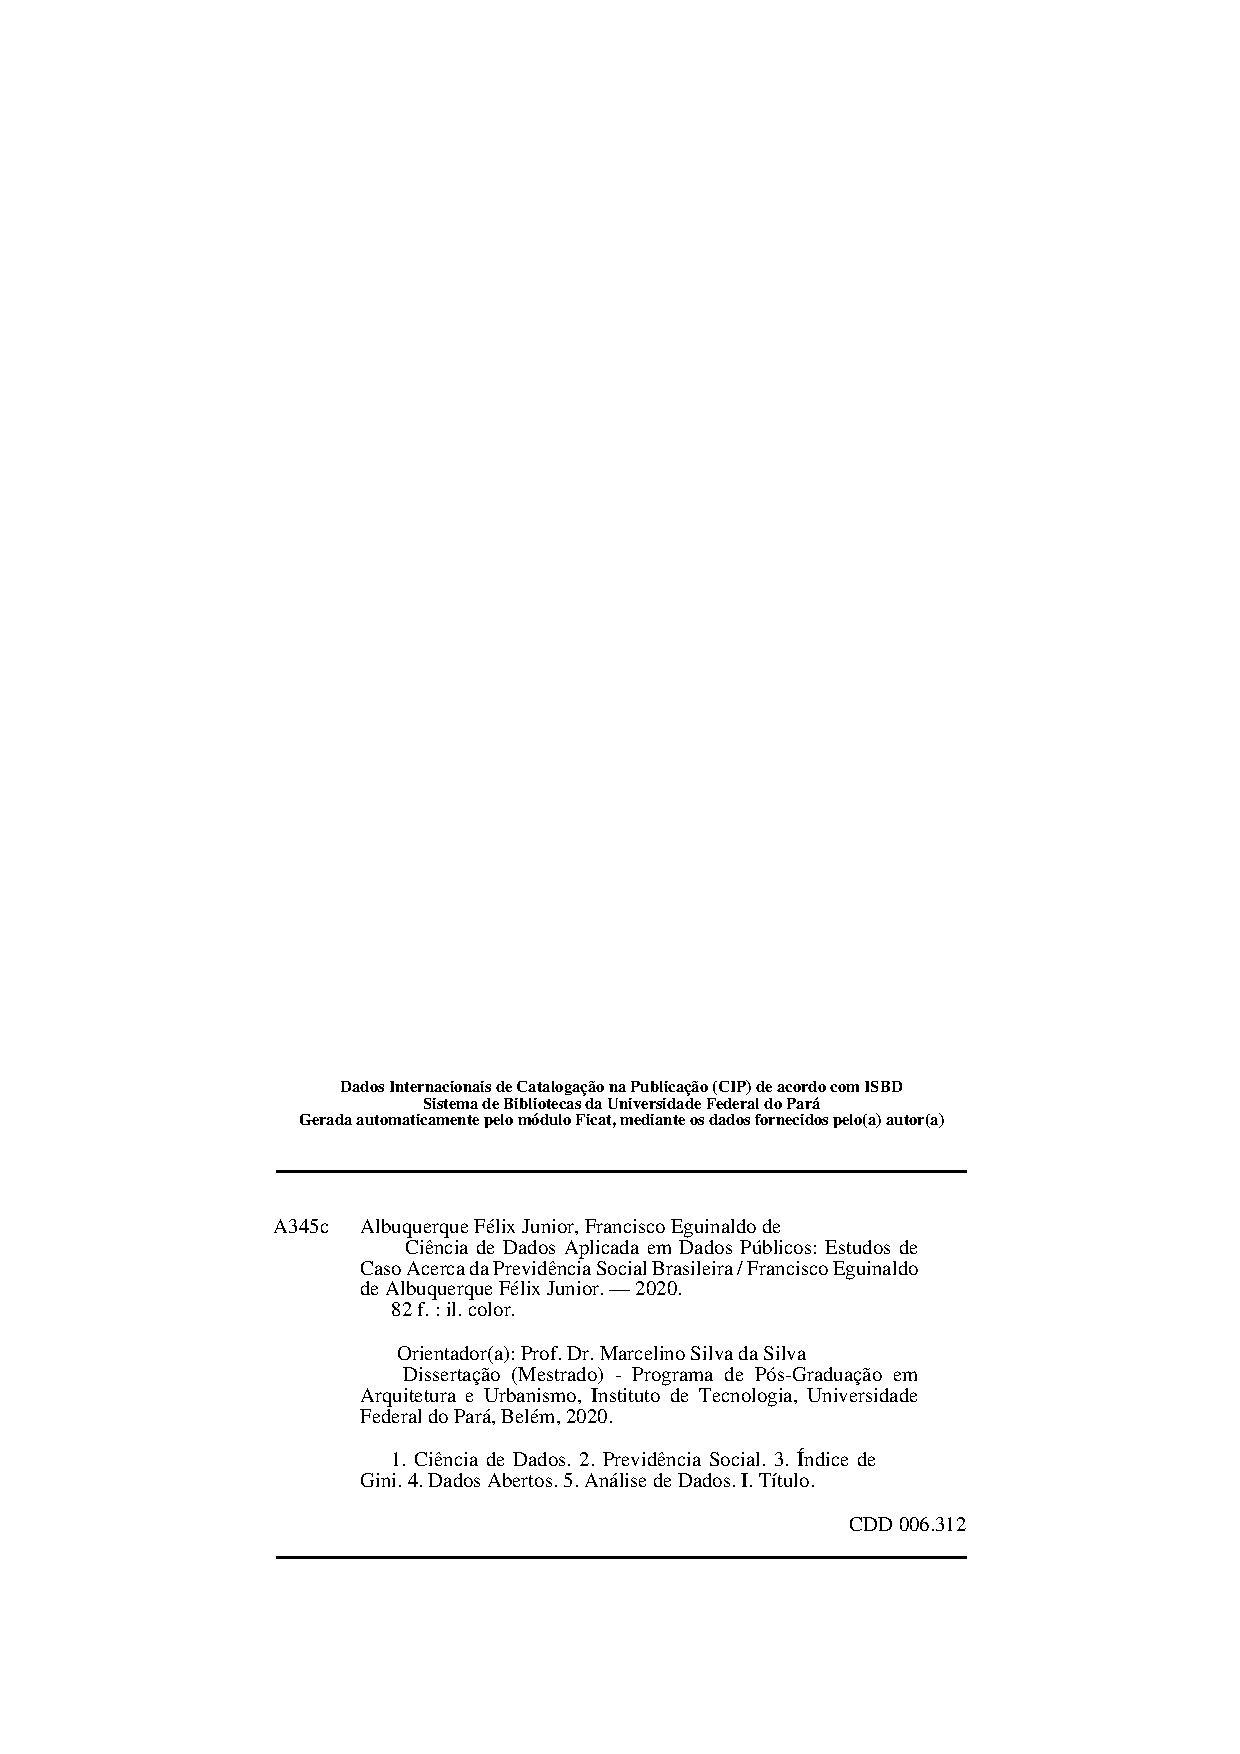
\includepdf[pages={1}]{pretextual/catalografica.pdf}

% Inserir Folha de Aprovação
% ---
% Assinaturas
% ---
% Isto é um exemplo de Folha de aprovação, elemento obrigatório da NBR
% 14724/2011 (seção 4.2.1.3). Você pode utilizar este modelo até a aprovação
% do trabalho. Após isso, substitua todo o conteúdo deste arquivo por uma
% imagem da página assinada pela banca com o comando abaixo:
%
% \includepdf{folhadeaprovacao_final.pdf}
%
\begin{folhadeaprovacao}

    \begin{center}
        {\large\imprimirautor}

        \vspace*{\fill}\vspace*{\fill}
        \begin{center}
            {\ABNTEXchapterfont\Large\textbf{\imprimirtitulo}}
        \end{center}
        \vspace*{\fill}
    \end{center}    
    
    Esta Dissertação foi julgada adequada para obtenção do título de Mestre em Engenharia Elétrica, e aprovada na sua forma final, pela banca examinadora, designada pelo Programa de Pós-Graduação em Engenharia Elétrica do Instituto de Tecnologia da Universidade Federal do Pará em 20 de Março de 2020.
    
%   \hspace{.45\textwidth}
%    \begin{minipage}{.5\textwidth}
%        \imprimirpreambulo
%    \end{minipage}%
%    \vspace*{\fill}
%   \end{center}
        
%   Trabalho aprovado. \imprimirlocal, 01 de janeiro de 2014:
    
   \vspace*{0.5cm}
   \textbf{Banca Examinadora:}
   
    \setlength{\ABNTEXsignwidth}{9cm}
    
   \assinatura{\footnotesize\textbf{\imprimirorientador} \\ Orientador} 
   % \assinatura{\textbf{\imprimircoorientador} \\ Co-Orientador} 
   \assinatura{\footnotesize\textbf{Prof. Dr. Diego Lisboa Cardoso} \\ Membro Interno - PPGEE UFPA}
   \assinatura{\footnotesize\textbf{Prof. Dr. Claudio Alberto Castelo Branco Puty} \\ Membro Externo - FACECON UFPA}
   \assinatura{\footnotesize\textbf{Prof. Dra. Liviane Ponte Rêgo} \\ Membro Externo - FACECON UFPA}

   \textbf{Visto:}
   \assinatura{\footnotesize\textbf{Prof. Dra. Maria Emília de Lima Tostes} \\ Coordenadora do PPGEE/ITEC/UFPA}
   
   \begin{center}

    \vspace*{0.5cm}
    {\large\imprimirlocal}
    \par
    {\large\imprimirdata}
    \vspace*{1cm}
  \end{center}
  
\end{folhadeaprovacao}
% ---

% Dedicatória
% ---
% Dedicatória
% ---
\begin{dedicatoria}
    \vspace*{\fill}
    \begin{flushright}
        \textit{ Aos meus pais \\
        Francisco Eguinaldo de Albuquerque Félix e Ivoneide Sales de Queiroz, \\ 
        por sempre estarem comigo em todos os momentos.}
   	\end{flushright}
\end{dedicatoria}
% ---


% Agradecimentos
% ---
% Agradecimentos
% ---
\begin{agradecimentos}

Primeiramente à Deus, por ter me dado saúde e forças para enfrentar e superar todas as dificuldades encontradas nessa trajetória.

Aos meus pais, Francisco Eguinaldo e Ivoneide Sales, que me incentivaram durante toda a minha vida e estiveram do meu lado em todos os momentos que precisei, prestando apoio e sempre me confortando com palavras de amor e confiança.

Ao meu orientador prof. Marcelino Silva, pelo suporte, ajuda, confiança para a elaboração do trabalho e pelos conselhos acadêmicos que vou levar
por toda a vida.

Aos meus amigos do LPO e LINC, Daniel Victor, Lucas, Ewerton, Sandio, Igor, Gean, Daniel Souza e Paulo que sempre me ajudaram nos trabalhos e dificuldades encontradas no dia a dia, em especial ao meu amigo André Augusto, companheiro no desenvolvimento desta pesquisa.

Aos professores que colaboraram para a minha formação acadêmica, em especial Fábio Lobato, Diego Lisboa, Cláudio Puty e Liviane Rêgo que sempre se dispuseram e estiveram presentes para me ajudar no desenvolvimento do trabalho.

À minha amiga Luanny Gomes, pela confiança, companheirismo, auxílio e colaboração na realização da minha pesquisa.

Aos meus amigos Max Weverton e Henrique Dias, pela parceria e ensinamentos de vida proporcionados no último ano.

À UFPA e ao PPGEE, por terem me acolhido como aluno de mestrado durante 2 anos, disponibilizando toda a infraestrutura necessária para a elaboração dessa dissertação. 

À CAPES pelo fomento da pesquisa realizada.

\end{agradecimentos}
%% ---

% Epígrafe
% ---
% Epígrafe
% ---
\begin{epigrafe}
    \vspace*{\fill}
	\begin{flushright}
		\textit{``A imaginação é mais importante que a ciência,\\
		porque a ciência é limitada, ao passo que a\\
		imaginação abrange o mundo inteiro.''\\ 
		(Albert Einstein)}
	\end{flushright}
\end{epigrafe}
% ---

% Resumo e Abstract
% ---
% RESUMOS
% ---

% RESUMO em português
\setlength{\absparsep}{18pt} % ajusta o espaçamento dos parágrafos do resumo
\begin{resumo}
A Ciência de Dados trata-se de uma área interdisciplinar relacionada a análise de dados, a qual, objetiva a extração de conhecimento e possíveis tomadas de decisão acerca de problemáticas especificas. Essa temática apresenta uma tendência evolutiva nos últimos anos devido, principalmente, a grande quantidade de dados não processados gerados cotidianamente, estimulando pesquisadores e empresas a realizarem estudos e análises cada vez mais complexas, propiciando avanços científicos nos mais variados campos, bem como, provendo vantagens competitivas às corporações. Nesse contexto, os dados abertos governamentais, por necessitarem recorrentemente de pré-tratamentos e métodos computacionais para processamento acerca dos seus conjuntos de dados, apresentam-se como potenciais fontes de informações a serem exploradas na ótica de Ciência de Dados, possibilitando o desenvolvimento de estratégias cada vez mais eficientes e otimizadas em gestão pública. Diante disso, e aliado as recentes discussões relacionadas a reforma na previdência social brasileira, essa dissertação apresenta dois estudos de caso referentes a análises no sistema previdenciário nacional. O primeiro estudo utilizou os microdados referentes aos censos demográficos de 2000 e 2010, disponibilizados pelo IBGE, propondo avaliar a participação que as aposentadorias e pensões possuem na desigualdade de renda da população nos anos avaliados acerca dos estados e municípios brasileiros. Para isso, foi aplicada a metodologia de decomposição do índice de Gini nesta parcela de benefícios, dividindo-os em categorias, até um salário mínimo e acima de um salário. Os resultados mostram que, embora os benefícios analisados contribuam para a concentração de renda no Brasil, a parcela correspondente até um salário mínimo contribui para a desconcentração da renda, e aquela acima de um salário contribui para a concentração, sendo um padrão repetitivo em todo o território nacional. Por outro lado, o segundo estudo propôs uma avaliação dos impactos que a reforma da previdência, proposta pela PEC 06/2019, causaria acerca das concessões dos benefícios de aposentadoria entre o período de 1995 a 2016. Para tal, foi desenvolvida uma estrutura de \textit{Data Warehouse} responsável por armazenar os microdados disponibilizados pela CPI da Previdência. Dessa forma, aplicando estratégias para processamento em lotes de dados e informações disponibilizadas pelo IBGE e AEPS, foram simuladas as regras previstas pela reforma acerca das aposentadorias concedidas no intervalo de tempo analisado. Após a simulação, observou-se que a PEC 06/2019 dificultaria o acesso aos benefícios, na qual, aproximadamente 83,28\% das aposentadorias não haveriam sido concedidas se a mesma já estivesse em vigor desde 1995.

\textbf{Palavras-chaves}: Ciência de Dados. Previdência Social. Índice de Gini. Dados Abertos. Análise de Dados.
\end{resumo}

% ABSTRACT in english
\begin{resumo}[Abstract]
 \begin{otherlanguage*}{english}
 Data Science is an interdisciplinary area related to data analysis, which aims to extract knowledge and possible decision-making about specific problems. This topic indicates an evolutionary trend in recent years, due to a large amount of unprocessed data generated daily, encouraging researchers and companies to carry out increasingly complex studies and analyses, assuring scientific advances in various fields, as well as insure competitive advantages on corporations. In this context, open government data, because they repeatedly need pre-treatments and computational methods to process their data sets, present themselves as potential sources of information to be explored taking the Data Science's perspective, allowing the development of strategies each time more efficient and optimized in public management. Given this, and allied to the recent discussions related to the reform in the Brazilian social security, this dissertation presents two case studies referring to analyzes in the national social security system. The first study used the microdata referring to the demographic censuses of 2000 and 2010, made available by IBGE, proposing to evaluate the participation that retirements and pensions have in the income inequality of the population in the years evaluated about Brazilian states and municipalities. For this, the Gini index decomposition methodology was applied to this portion of benefits, dividing them into categories, lower or equal to one minimum wage and above one minimum wage. The results show that, although the analyzed benefits contribute to the Brazil income concentration, the portion corresponding to a minimum wage contributes to the deconcentration of income, and the portion above one salary contributes to the concentration, being a repetitive pattern throughout the country. On the other hand, the second study proposed an evaluation of the impacts caused by the pension reform, which is proposed in PEC 06/2019, For this, a \textit{Data Warehouse} structure was developed, responsible for storing the microdata provided by the Social Security CPI. Thus, applying data batch processing strategies and using the information provided by IBGE and AEPS, was simulated the rules predicted by the reform regarding the pensions granted in the analyzed time interval. After the simulations, it was observed that PEC 06/2019 would hinder access to benefits, in which approximately 83,28\% of the pensions would not have been granted had it been in effect since 1995.

\vspace{\onelineskip}
 
\noindent 
\textbf{Keywords}: Data Science. Social Security. Retirements. Gini Index. Open Data. Data Analysis.
\end{otherlanguage*}
\end{resumo}

% Lista de ilustrações
\pdfbookmark[0]{\listfigurename}{lof}
\listoffigures*
\cleardoublepage

% Lista de tabelas
\pdfbookmark[0]{\listtablename}{lot}
\listoftables*
\cleardoublepage

% Lista de abreviaturas e siglas
\begin{siglas}
    \item[\textbf{AEPS}] Anuário Estatístico da Previdência Social
    \item[\textbf{AMC}] Área Mínimas Comparáveis
    \item[\textbf{ANFIP}] Associação Nacional dos Auditores Fiscais da Receita Federal
    \item[\textbf{BI}] Business Intelligence
    \item[\textbf{CPI}] Comissão Parlamentar de Inquérito
    \item[\textbf{ETL}] Extract, Transfom and Load
    \item[\textbf{GPL}] General Public License
    \item[\textbf{IBGE}] Instituto Brasileiro de Geografia e Estatística
    \item[\textbf{INCP}] Índice Nacional de Preços ao Consumidor
    \item[\textbf{INSS}] Instituto Nacional de Seguro Social
    \item[\textbf{KDD}] Knowledge-Discovery in Database
    \item[\textbf{LAI}] Lei de Acesso à Informação
    \item[\textbf{LDO}] Lei de Diretrizes Orçamentarias
    \item[\textbf{MD}] Mineração de Dados
    \item[\textbf{ONU}] Organização das Nações Unidas
    \item[\textbf{PAYG}] Pay As You Go
    \item[\textbf{PDI}] Pentaho Data Integration
    \item[\textbf{PEC}] Proposta de Ementa Constitucional
    \item[\textbf{PIB}] Produto Interno Bruto
    \item[\textbf{PNAD}] Pesquisa Nacional por Amostra de Domicílios
    \item[\textbf{RD}] Rendimento Domiciliar
    \item[\textbf{RGPS}] Regime Geral da Previdência Social
    \item[\textbf{SGBD}] Sistema Gerenciador de Banco de Dados
    \item[\textbf{SQL}] Structured Query Language
\end{siglas}

% Lista de símbolos
%\begin{simbolos}
%  \item[$ \Gamma $] Letra grega Gama
%  \item[$ \Lambda $] Lambda
%  \item[$ \zeta $] Letra grega minúscula zeta
%  \item[$ \in $] Pertence
%\end{simbolos}

% Inserir o SUMÁRIO
\pdfbookmark[0]{\contentsname}{toc}
\renewcommand{\tocheadstart}{{\fontfamily{lmr}}}
\tableofcontents*
\cleardoublepage

% ----------------------------------------------------------
% ELEMENTOS TEXTUAIS (Capítulos)
% ----------------------------------------------------------
\textual
% Elementos textuais com numeração arábica
\pagenumbering{arabic}
% Reinicia a contagem do número de páginas
\setcounter{page}{1}

% Inclui cada capitulo da Dissertação
% ----------------------------------------------------------
% Introdução 
% Capítulo sem numeração, mas presente no Sumário
% ----------------------------------------------------------

\chapter{Introdução}

A Previdência Social é um programa de seguro público responsável por manter a fonte de renda dos trabalhadores e suas famílias quando estes perdem suas capacidades laborais provisoriamente, por acidentes, doenças ou maternidade, ou permanentemente, devido a morte, invalidez ou velhice. Esse programa é encarregado pelo ressarcimento de diversos benefícios sociais do trabalhador brasileiro, tais como aposentadorias, auxílios-doença, auxílios-acidente, pensão por morte, dentre outros \cite{cap04_ref6}. No cenário brasileiro, os trabalhadores formais, correspondentes aqueles que possuem carteira assinada, financiam mensalmente o fluxo de caixa dos repasses previdenciários, sendo comumente conhecido como regime de repartição simples ou \textit{pay as you go} (PAYG). O Regime Geral da Previdência Social (RGPS), responsável por atender os trabalhadores da iniciativa privada e aos servidores públicos que não contam com regimes próprios de previdência, estrutura-se nesse modelo de repartição \cite{cap05_ref11}.

Os segurados da Previdência Social necessitam, como pré-requisito mínimo, contribuir regularmente para o Instituto Nacional do Seguro Social (INSS). Esse corresponde a uma autarquia do Governo Federal vinculado ao Ministério da Economia, possuindo como principal responsabilidade organizar as arrecadações e pagamentos dos benefícios previdenciários previstos por lei \cite{cap01_ref1}. O INSS trabalha em parceria com Empresa de Tecnologia e Informações da Previdência, o DATAPREV, encarregada por realizar o armazenamento e processamento dos dados gerados pelo instituto \cite{cap01_ref2}.

Avaliando a Previdência Social em uma ótica mundial, observa-se em diversos países a realização de modificações em seus sistemas previdenciários tradicionais. Tais medidas, na maior parte das vezes, envolvem um acréscimo no tempo mínimo de contribuição e idade mínima como requisitos para acesso aos benefícios. Essas reformas, comumente, justificaram-se em uma relação de proporcionalidade entre as variáveis demográficas e financeiras, ou seja, o aumento da expectativa de vida e estagnação na densidade de população economicamente ativa proporcionaria gastos com beneficiários maiores do que arrecadações. Dessa forma, esse novo perfil etário causaria um desequilíbrio nas contas do sistema previdenciário \cite{cap01_ref3, cap03_ref5}. 

Nesse contexto, a Organização das Nações Unidas (ONU) projeta que até 2100 a população idosa do mundo, correspondente a pessoas acima de 60 anos, tende a triplicar, estimando que essa categoria da população ultrapasse 3 bilhões de habitantes \cite{cap05_ref4}. A nível nacional, de acordo com o Instituto Brasileiro de Geografia e Estatística (IBGE), os índices de longevidade apresentam-se progressivos para os próximos anos convergindo para um crescente envelhecimento populacional \cite{cap05_ref5}.

\section{Motivação e Justificativa}

Atualmente, um dos assuntos mais discutidos no cenário político brasileiro refere-se a uma reforma na Previdência Social a qual ganhou destaque novamente no final do ano de 2016. Devido à natureza macroeconômica desse tema, diversos debates foram acarretados acerca da sua dimensão econômica-fiscal, por compreender uma significativa parcela dos orçamentos públicos, e do seu caráter político-social, por refletir diretamente em mudanças nas regras previdenciárias sobre um conjunto grande da população, incluindo contribuintes/segurados e beneficiários. 

Dessa forma, o governo federal, motivado pela desaceleração do crescimento econômico e elevação da dívida pública \cite{cap05_ref6}, justificou a necessidade dessa reforma argumentando que, devido as elevadas taxas de longevidade registradas, o atual sistema tende a se tornar insustentável no decorrer dos próximos anos, e que Previdência Social pressiona a carga tributária nacional diminuindo o espaço para outros setores na composição do gasto público \cite{cap05_ref7}. Com isso, foi apresentada a população brasileira a Proposta de Ementa Constitucional n. 287 de dezembro de 2016 (PEC 287/16) – posteriormente substituída pela PEC 06/2019 devido ao seu insucesso – propondo alterações nas regras previdenciárias em idade mínima e tempo de contribuição para acesso aos benefícios. Destaca-se que entre os itens da reforma as principais modificações ocorrem no RGPS.

Embora diversos cálculos atuarias estejam sendo realizados a fim de estimar, a curto e longo prazo, a solvência do sistema previdenciário atual \cite{cap01_ref1, cap01_ref4}, é necessário ponderar acima de tudo o impacto social que tais alterações acarretariam. Mediante a isso, o Ministério da Fazenda, através da Comissão Parlamentar de Inquérito (CPI) da Previdência, divulgou em junho de 2017 bases de dados relacionados aos números de benefícios de aposentadorias concebidos pelo RGPS, com o intuito de possibilitar a investigação dos resultados divulgados pelo programa.

Paralelamente, o advento da ciência de dados tem ganhado destaque no cenário interdisciplinar com a crescente densidade de informações geradas pelos diversos segmentos da sociedade \cite{cap01_ref5}. Tal fator possibilita, sobretudo, o desenvolvimento de um novo campo de estudo para análises, simulações de cenários e extração de conhecimento válido acerca de bases de dados públicas. Nesse contexto, a utilização dos microdados previdenciários aliados a outras fontes de informação - demográficas e sociais - motivou o desenvolvimento dessa pesquisa, visto que possibilita a realização de avaliações críticas acerca do efeito que as aposentadorias causam na população brasileira e das consequências sociais que uma possível reforma nas regras para acesso aos benefícios causaria.

\section{Objetivos Geral e Específicos}

Diante disso, esta pesquisa objetiva, de forma geral, explorar a aplicação de técnicas e estratégias de Ciência de Dados em Dados Abertos Governamentais da Previdência Social. Para tanto, foram realizados dois estudos de caso visando: estimar a participação que o sistema previdenciário possui no cenário socioeconômico nacional; e simular os impactos que a reforma prevista na PEC 06/2019 causaria nas concessões de aposentadorias. 

Especificamente, essa pesquisa tem como objetivos:

\begin{itemize}
    \item Utilizar os microdados dos censos demográficos de 2000 e 2010, disponibilizados pelo IBGE, e metodologia de decomposição do coeficiente de Gini, para aferir matematicamente a participação das aposentadorias e pensões na distribuição de renda da população brasileira a nível estadual e municipal.
    
    \item Modelar uma estrutura de \textit{Data Warehouse} para armazenar os microdados oficiais disponibilizados pela CPI da Previdência de 2017, objetivando - a partir da utilização de técnicas de processamento em lotes - simular os efeitos que a PEC 06/2019 causaria no cenário previdenciário entre 1995 a 2016, se a mesma já estivesse em vigor no momento em que cada benefício foi concedido.
    
    \item Aplicar estratégias e conceitos de ciência de dados para o tratamento, organização e processamento dos microdados utilizados, visando possibilitar a extração de conhecimento válido com simulações ou aplicação de medidas estatísticas acerca dos resultados gerados em cada análise proposta.
\end{itemize}

\section{Organização da Dissertação}

Este trabalho está organizado da seguinte forma:

\begin{itemize}
    \item Capítulo 1: apresenta uma breve introdução do assunto abordado, a motivação para realização dessa pesquisa e os objetivos, geral e específicos, propostos por essa dissertação.
    
    \item Capítulo 2: apresenta a fundamentação teórica que norteou essa pesquisa, destacando os conceitos de análise de dados, ciência de dados e dados abertos, além de elencar os principais modelos matemáticas utilizados nas análises propostas.
    
    \item Capítulo 3: elenca os principais trabalhos correlatos a essa pesquisa, apontando as contribuições desta dissertação perante ao estado da arte da problemática abordada.
    
    \item Capítulo 4: apresenta o primeiro estudo de caso desta dissertação, responsável por avaliar a participação que as aposentadorias e pensões possuem na distribuição de renda da população brasileira.
    
    \item Capítulo 5: apresenta o segundo estudo de caso desta dissertação, responsável por simular os impactos que a reforma previdenciária prevista pela PEC 06/2019, avaliando o período de 1995 a 2016, causaria acerca das concessões de benefícios na hipótese da mesma já está em vigor quando cada aposentadoria foi concedida.
    
    \item Capítulo 6: apresenta as considerações finais desta pesquisa e as perspectivas de trabalhos futuros acerca dos estudos realizados.
\end{itemize}




\chapter{Referencial Teórico}\label{cap:referencias}

% --------------------------------------------------------------------------- %
\section{Considerações Iniciais}

Este capítulo tem como finalidade conceituar teoricamente as aplicações e técnicas que fundamentaram a realização deste trabalho. Serão abordadas as definições de análise de dados e ciência de dados, destacando suas importâncias perante o cenário cientifico e tecnológico, além de conceituar o seu emprego na elaboração e organização de conjuntos de dados como os que nortearam o presente estudo. Também será abordada a importância das bases de dados governamentais disponibilizadas pelos órgãos públicos, finalizando o capítulo com uma fundamentação das técnicas matemáticas aplicadas nesta pesquisa.

% --------------------------------------------------------------------------- %
\section{Análise de Dados}

Com a evolução de novas e mais modernas tecnologias, aliada ao advento da Internet e das mídias sociais, uma enorme quantidade de dados está sendo gerada e coletada diariamente a uma velocidade cada vez maior \cite{cap02_ref7, cap02_ref10}. Celulares, notebooks, equipamentos hospitalares, automóveis, sensores, câmeras de segurança e diversos outros dispositivos eletrônicos presentes nos mais diversos segmentos da sociedade geram automaticamente informações que precisam ser armazenadas e muitas vezes processadas em tempo real. Entretanto, acompanhar, analisar e extrair conhecimento acerca desse fluxo de dados é uma tarefa substancialmente desafiadora, especialmente quando estes não estão em conformidade com as noções tradicionais de estrutura de dados \cite{cap02_ref3}.

Tal fenômeno, além de estar cada vez mais inserido no cotidiano da população, tem apresentado um crescimento exponencial. Segundo \cite{cap02_ref4} aproximadamente 90\% dos dados existentes no mundo foram criados nos últimos 2 anos\footnote{Informações referentes ao ano de 2016.}. Adicionalmente, o barateamento de ferramentas computacionais com maior poder de processamento e a onipresença da rede estão colaborando para que pessoas e empresas desenvolvam algoritmos acerca desses dados nas mais diversas áreas do conhecimento como: economia, engenharia, sociologia, saúde, marketing, dentre outras \cite{cap02_ref9, cap02_ref5}

Diante desse cenário, a utilização de técnicas computacionais para a aquisição inteligente de conhecimento acerca de dados sem representatividade passou a ser uma tarefa cada vez mais atrativa, uma vez que muda a forma como tais dados são analisados e contextualizados \cite{cap02_ref11}. Desse modo, Mineração de Dados (MD), Extração de Conhecimento de Base de Dados (mais conhecida como \textit{Knowledge-Discovery in Database} – KDD) e Inteligência de Negócios (do inglês \textit{Business Inteligence} – BI) são exemplos de métodos ou estratégias que buscam extrair informações e identificar padrões/tendências para a resolução de problemas específicos acerca de conjunto de dados \cite{cap02_ref12, cap02_ref4}. 

Embora diversos autores interpretem os processos KDD e MD como sinônimos \cite{cap02_ref11, cap02_ref6}, boa parte da literatura considera a mineração como uma etapa da descoberta de conhecimento, sendo essa composta pela seleção, pré-processamento, transformação, mineração de dados e interpretação \cite{cap02_ref12, cap02_ref5}. A Figura~\ref{fig:kdd_process} elenca as etapas necessárias para a extração de conhecimento.


\begin{figure}[htpb]
   \centering
   \caption{Processo de descoberta de conhecimento em bases de dados.}
   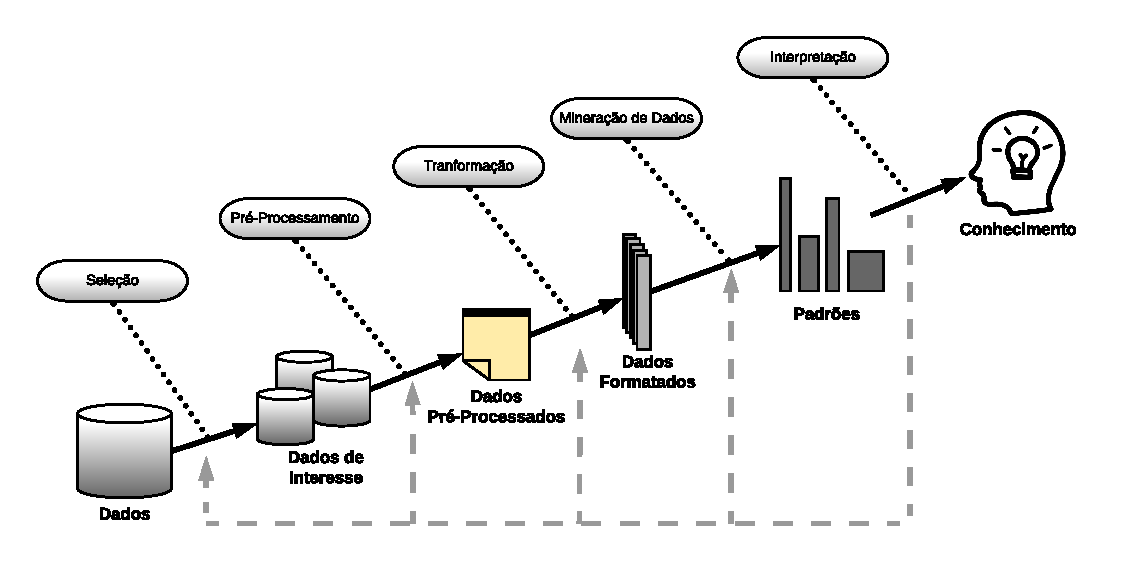
\includegraphics[width=0.7\textwidth]{figs/cap02_KDD_model.png}
   \caption*{\footnotesize{Fonte: \cite{cap02_ref11}}}
   \label{fig:kdd_process}
\end{figure}

A primeira fase do KDD é compreendida pelo conhecimento do domínio, ou identificação do problema, responsável por, a partir de avalição do domínio da aplicação a qual os dados pertencem, compreender e avaliar o processo como um todo e definir as metas e objetivos a serem alcançados. A segunda etapa é de fundamental importância para a realização de uma extração de conhecimentos válidos e potencialmente uteis sendo denominada de pré-processamento. Esta demanda aproximadamente 80\% do tempo total do processo \cite{cap02_ref13}, e é responsável pela limpeza, correção de dados que ausentes, errôneos ou inconsistentes e possíveis transformações, objetivando facilitar posteriores identificações de padrões.
Posteriormente, no estágio de extração de padrões, ocorre a aplicação de algoritmos de Mineração de Dados específicos para o reconhecimento de padrões ou tendências acerca do conjunto de dados avaliado. \cite{cap02_ref5} destaca 4 tipos de técnicas de inteligência computacional para a realização dessas propostas: 
\begin{itemize}
    \item Classificação: prediz a qual categoria ou classe um determinado item do conjunto de dados pertence;
    \item Agrupamento: também conhecido como \textit{clustering}, identifica grupos de itens com propriedades e características semelhantes sem pressupor classes especificas;
    \item Associação: identifica grupos de dados que apresentem correlaçãoão entre si;
    \item Regressão: utiliza uma função preditiva para mapear valores associados aos dados em um ou mais valores reais.
\end{itemize}

Perante aos diversos algoritmos de mineração de dados existente, a seleção da estratégia especifica a ser utilizada não é uma tarefa trivial. Algumas das técnicas descritas acima consiste na aplicação de um determinado algoritmo enquanto outras propõe a utilização de diversos métodos objetivando uma maior confiabilidade no resultado final. Portanto, para a seleção do algoritmo apropriado, deve-se levar em consideração o objetivo final da análise ponderando possíveis hipóteses \cite{cap02_ref14}.
Em seguida, é realizada a etapa de pós-processamento acerca dos resultados encontrados. O sucesso dessa etapa determina a eficácia de todo o processo de KDD, avaliando e validando as informações geradas afim de identificar possíveis falhas nas fases anteriores \cite{cap02_ref12}. Observando a Figura~\ref{fig:kdd_process}, é possível observar que o fluxo do KDD é um processo recursivo, ou seja, caso o resultado encontrado seja incoerente ou não aceitável é possível reiniciar o mesmo, analisando todas as etapas em busca de melhorar e/ou refazer o que for necessário, até que o conhecimento resultante seja julgado como satisfatório.


De forma semelhante, o processo de BI tem como finalidade coletar, organizar, compartilhar e analisar grandes volumes de dados empresariais projetando a realização de estratégias em gestão de negócios que visem a obtenção de vantagens competitivas \cite{cap02_ref16, cap02_ref15}. Tal procedimento, embora tenha uma metodologia própria, se assemelha bastante a técnica de KDD visto que ambos objetivam a extração de conhecimento válido acerca de conjuntos de dados \cite{cap02_ref17}. 

No entanto, devido a diversos fatores históricos, como o crescente acumulo de dados, aumento da interdisciplinaridade das problemáticas abordadas, e até mesmo necessidade de padronização de uma área específica que englobe as diferentes vertentes de análises de dados, houve o surgimento de um novo campo de estudo, conhecido como ciência de dados \cite{cap02_ref2, cap02_ref9, cap02_ref33, cap02_ref32}, tema abordado na próxima seção.

% --------------------------------------------------------------------------- %
\section{Ciência de Dados}

Ciência de dados, do inglês \textit{data science}, corresponde a uma área interdisciplinar relacionada a análise de dados que objetiva a extração de conhecimento, e possíveis tomadas de decisões, acerca de problemáticas especificas \cite{cap02_ref1, cap02_ref4}. Embora tal conceito seja similar aos de KDD e BI, a ciência de dados pode ser compreendida como um domínio de estudo mais abrangente, englobando todas as definições e técnicas computacionais abordadas anteriormente em um novo campo de pesquisa \cite{cap02_ref2}.

Em relação a definição de ciência de dados, observa-se no estado da arte dessa temática uma dificuldade na sua conceituação formal. Para \cite{cap02_ref33}, por exemplo, essa área pode ser entendida como um campo científico que desenvolve tecnologias e teorias relevantes para dados, desde a sua extração, pré-processamento, representação, armazenamento, pesquisa, compartilhamento, segurança, modelagem, aprendizagem, análise e visualização, até a sua integração com recursos heterógeneos, complexos e interdependentes para tomadas de decisão e abstração de valores significativos.

Por outro lado, de acordo com \cite{cap02_ref34}, a ciência de dados compreende praticamente tudo que tenha alguma relação com dados, desde a sua coleta até possíveis análises e modelagens. Contudo, destaca-se como um dos seus requisitos básicos a necessidade de aplicações desses dados na resolução de problemas, dos mais simples aos mais complexos, utilizando como instrumentos para auxilio técnicas matemáticas, ferramentas computacionais e avaliações críticas acerca das problemáticas abordadas. Além disso, a criatividade e intuição para elaborar a visualização dos resultados, também conhecido como \textit{data visualization}, caracterizam os estudos associados a ciência de dados \cite{cap02_ref18}.

Outra abordagem para ciência de dados é compreendida pela agregação de três competências, ou áreas, básicas do campo científico: ciência da computação, matemática e estatística e a especialização cientifica da problemática em questão \cite{cap02_ref2}. A Figura~\ref{fig:veen_diagram} ilustra um diagrama de \textit{venn} contendo tais competências e suas inter-relações, enfatizando a ciência de dados como um novo campo de estudo sendo produto de todas as áreas relatadas.

\begin{figure}[!h]
   \centering
   \caption{Competências fundamentas para Ciência de Dados.}
   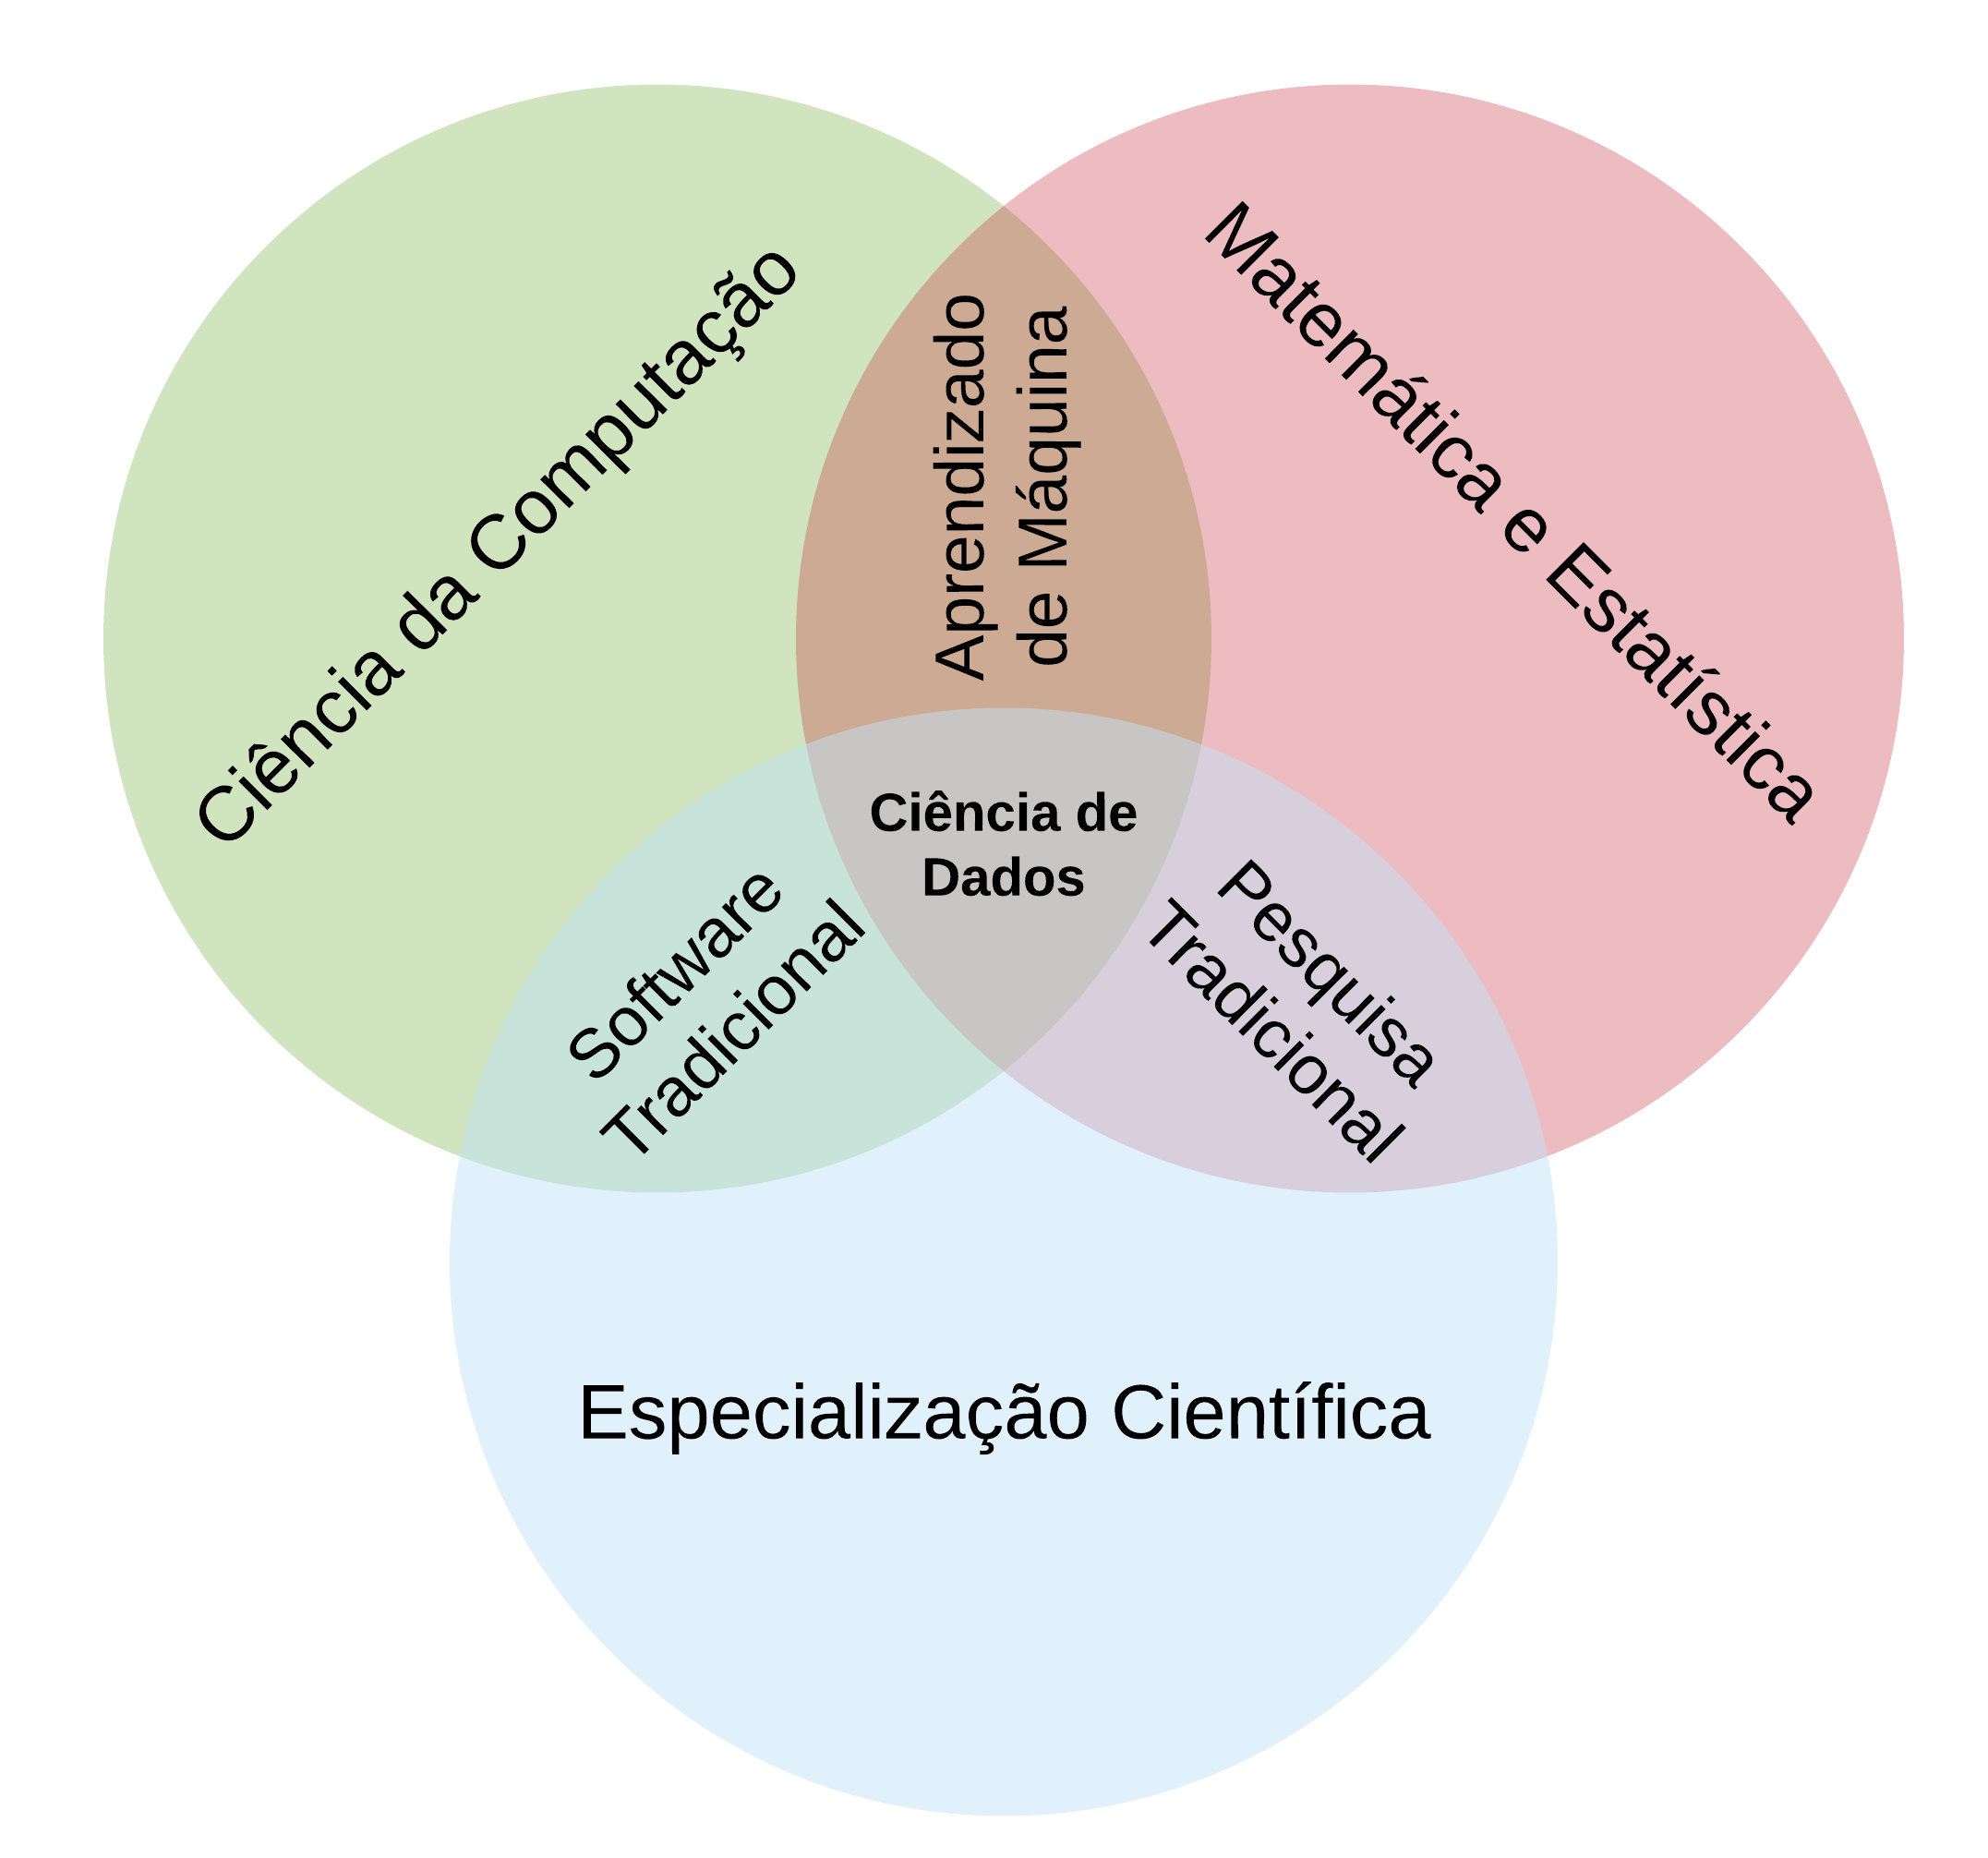
\includegraphics[width=0.55\textwidth]{figs/cap02_diagrama_veen_ds.png}
   \caption*{\footnotesize{Fonte: Adaptado de \cite{cap02_ref2}}}
   \label{fig:veen_diagram}
\end{figure}

A respeito da utilização de ciência de dados, a pesquisa de \cite{cap02_ref35} destaca que, embora o emprego de sistemas avançados de inteligência artificial mostre-se promissores em estratégias de negócios, a maioria das empresas não encontram-se preparadas para implementar tal abordagem. De acordo com a autora, há uma hierarquia de necessidades, nas quais, requisitos básicos necessitam ser atendidos antes de obter possíveis benefícios a partir da utilização de modelos de inteligência artificial. Contudo, destaca-se que a aplicação de análises estatísticas simples ou extração de características acerca dados sem representatividade podem ser compreendidas como aplicações da ciência de dados. 

Embora as principais aplicações da ciência de dados estejam fortemente relacionadas ao setor econômico e financeiro, devido principalmente ao fato de ter nascido neste ambiente para a resolução da problemática de grande quantidade de dados geradas pelas empresas \cite{cap02_ref9}, a utilização desta área nos desafios encontrados pela pesquisa científica tornou-se uma alternativa plausível em virtude, essencialmente, da sua capacidade adaptativa e interdisciplinar \cite{cap02_ref2}.

% --------------------------------------------------------------------------- %
\section{Dados Abertos}

O conceito de dados abertos, do inglês \textit{open data}¸ faz referência a dados que podem ser utilizados, reutilizados ou redistribuídos livremente por qualquer pessoa, restringindo, no máximo, a atribuição à fonte original e ao compartilhamento das mesmas licenças em que as informações foram apresentadas \cite{cap02_ref25}. Dessa forma, a abertura de dados objetiva restringir o controle e restrições existentes em dados que forem publicados, possibilitando a exploração dos seus conteúdos de forma livre por pessoas (sejam essas físicas ou jurídicas) \cite{cap02_ref24}. 

Assim sendo, em \cite{cap02_ref26} o conceito de dados abertos é compreendido por três normas fundamentais:

\begin{itemize}
    \item Os dados devem ser disponibilizados em um meio acessível, preferencialmente na internet, em um formato compreensível por máquina de tal forma que este possa ser acessado e modificado.
    
    \item Os dados devem ser disponibilizados perante a termos que permitam sua reutilização e redistribuição, inclusive a combinando com outros conjuntos de dados.
    
    \item Todos os usuários devem ser capazes de utilizar, reutilizar e redistribuir os dados, sem haver discriminação com áreas de atuação, pessoas ou grupos.
\end{itemize}

Uma vez que o movimento de dados abertos é estimulado e que as três regras supracitadas são atendidas, é aberta a possibilidade que diferentes pessoas, organizações e sistemas trabalhem de forma colaborativa. Tal fator é justificado pela interoperação dos dados que foram abertos, ampliando a comunicação existente e potencializando o desenvolvimento de sistemas cada vez mais complexos \cite{cap02_ref24}.

É importante ressaltar que os dados abertos não correspondem somente aqueles divulgados pelo governo, podendo originar de qualquer instituição contanto que atenda os requisitos básicos citados anteriormente, não apresentando restrições de uso \cite{cap02_ref37}. Existem casos de dados abertos disponibilizados por diversas industrias ou setores, como transporte, produtos, sustentabilidade, mapas, economia, cultura, finanças, negócios, entre outros. A Figura~\ref{fig:dadosabertos} apresenta alguns exemplos de tipos de dados abertos comumente encontrados na internet \cite{cap02_ref36}.

\begin{figure}[!h]
   \centering
   \caption{Tipos de dados abertos}
   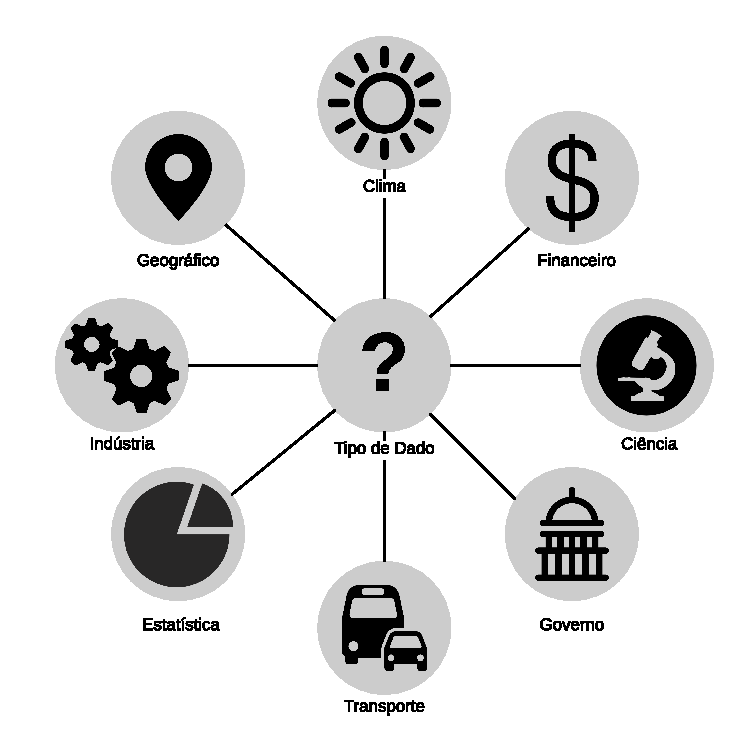
\includegraphics[width=0.75\textwidth]{figs/cap02_dados_abertos.pdf}
   \caption*{\footnotesize{Fonte: Adaptado de \cite{cap02_ref36}}}
   \label{fig:dadosabertos}
\end{figure}

\subsection{Dados Abertos Governamentais}

O conceito de dados abertos governamentais está sendo cada vez mais disseminado, sobretudo após a divulgação de um memorando em 2008 do até então presidente dos Estados Unidos Barack Obama \cite{cap02_ref27}. Neste, é discutida a transparência de dados governamentais norte-americanos através da criação de uma plataforma web \cite{cap02_ref28} que disponibilizasse dados abertos para qualquer cidadão.

A abertura dos dados públicos objetiva, sobretudo, estimular que a sociedade desenvolva produtos, serviços e novas atividades econômicas utilizando essas informações. Além disso, destacam-se benefícios políticos relacionados, principalmente, a transparência governamental gerada através do acompanhamento das elaborações de políticas públicas. Tal fator, além de intensificar a responsabilidade e participação democrática dos cidadãos, aumenta a confiabilidade transmitida pelo governo \cite{cap02_ref38}.

Nesse cenário, o governo brasileiro apresenta-se como um dos fundadores do \textit{Open Government Partnership} \cite{cap02_ref30} em 2011, uma iniciativa internacional que visa a promoção de governos abertos através da capacitação de cidadãos, combate a corrupção e aproveitamento de novas tecnologias. Além disso, a política de dados abertos governamentais no Brasil é consolidada pela Lei n. 12.527 de 2011, conhecida como Lei de Acesso à Informação (LAI), a qual garante acesso a qualquer informação de interesse público, desde que esta não seja imprescindível a segurança da sociedade e do Estado \cite{cap02_ref31}. De maneira similar aos Estados Unidos, no Brasil há uma plataforma de acesso aos dados abertos governamentais \cite{cap02_ref29}, sendo um portal que disponibiliza informações públicas seguindo os princípios de dados abertos relatados anteriormente.

No entanto, embora os dados abertos governamentais apresentem impactos extremamente positivos no governo, na sociedade e na economia, evidenciam-se adversidades relacionadas a sua implantação. Nesse contexto, o trabalho de \cite{cap02_ref38} divide esses obstáculos em seis grandes grupos: institucionais, complexidade da tarefa, utilização, legislação, qualidade da informação e técnicas. Dessa forma, a estimulação para a participação da população no uso dessas fontes de informações apresenta-se potencialmente promissora acerca das vantagens abordadas nessa subseção.

% --------------------------------------------------------------------------- %
\section{Técnicas Matemáticas Utilizadas}
\subsection{Decomposição do Índice de Gini}\label{cap:referencias:gini}

O índice de Gini, também conhecido como coeficiente de Gini, é uma medida de dispersão estatística elaborado pelo italiano Corrando Gini que objetiva mensurar o grau de desigualdade de uma variável acerca de um conjunto de dados \cite{cap02_ref19, cap02_ref20}. Esse indicador é fortemente utilizado em econômica para aferir o grau de desigualdade de renda da população, no entanto, é possível aplicá-lo em diversos campos de estudo como educação, ecologia, ciências da saúde, sociologia, dentre outros \cite{cap02_ref23}. Sua interpretação baseia-se em um número variado entre 0 e 1, no qual 0 corresponde a total igualdade (todos recebem a mesma renda) e 1 a total desigualdade (uma pessoa detém de toda renda e os demais nada) \cite{cap02_ref19, cap02_ref21}.

Matematicamente, assume-se uma série discreta $x_i (i, ..., n)$ correspondente a renda da $i$-ésima pessoa de uma população com $n$ pessoas. Admite-se que as rendas estão ordenadas, sendo:

\begin{equation} 
    x_1 \leq x_2 \leq ... \leq x_i \leq ... \leq x_n
    \label{eq:2.1}
\end{equation}

Agregando as pessoas da mais pobre até a i-ésima posição da série~\ref{eq:2.1}, a proporção acumulada da população é dada por:

\begin{equation}
    p_{i} = \frac{i}{n}
\end{equation}

\noindent e a respectiva para proporção acumulada de renda é:

\begin{equation}
    \varphi_i = \frac{1}{n \mu} \sum_{j=1}^{i} x_j
\end{equation}

\noindent onde $\mu$ é a renda média, dada por:

\begin{equation}
    \mu = \frac{1}{n} \sum_{i=1}^{n} x_i
\end{equation}

A Curva de Lorenz é obtida pela relação entre os pares ordenados dos valores de $p_i$ e $\varphi_i$, conforme indicado na Figura~\ref{fig:lorenz_curve}.

\begin{figure}[!h]
   \centering
   \caption{Curva de Lorenz}
   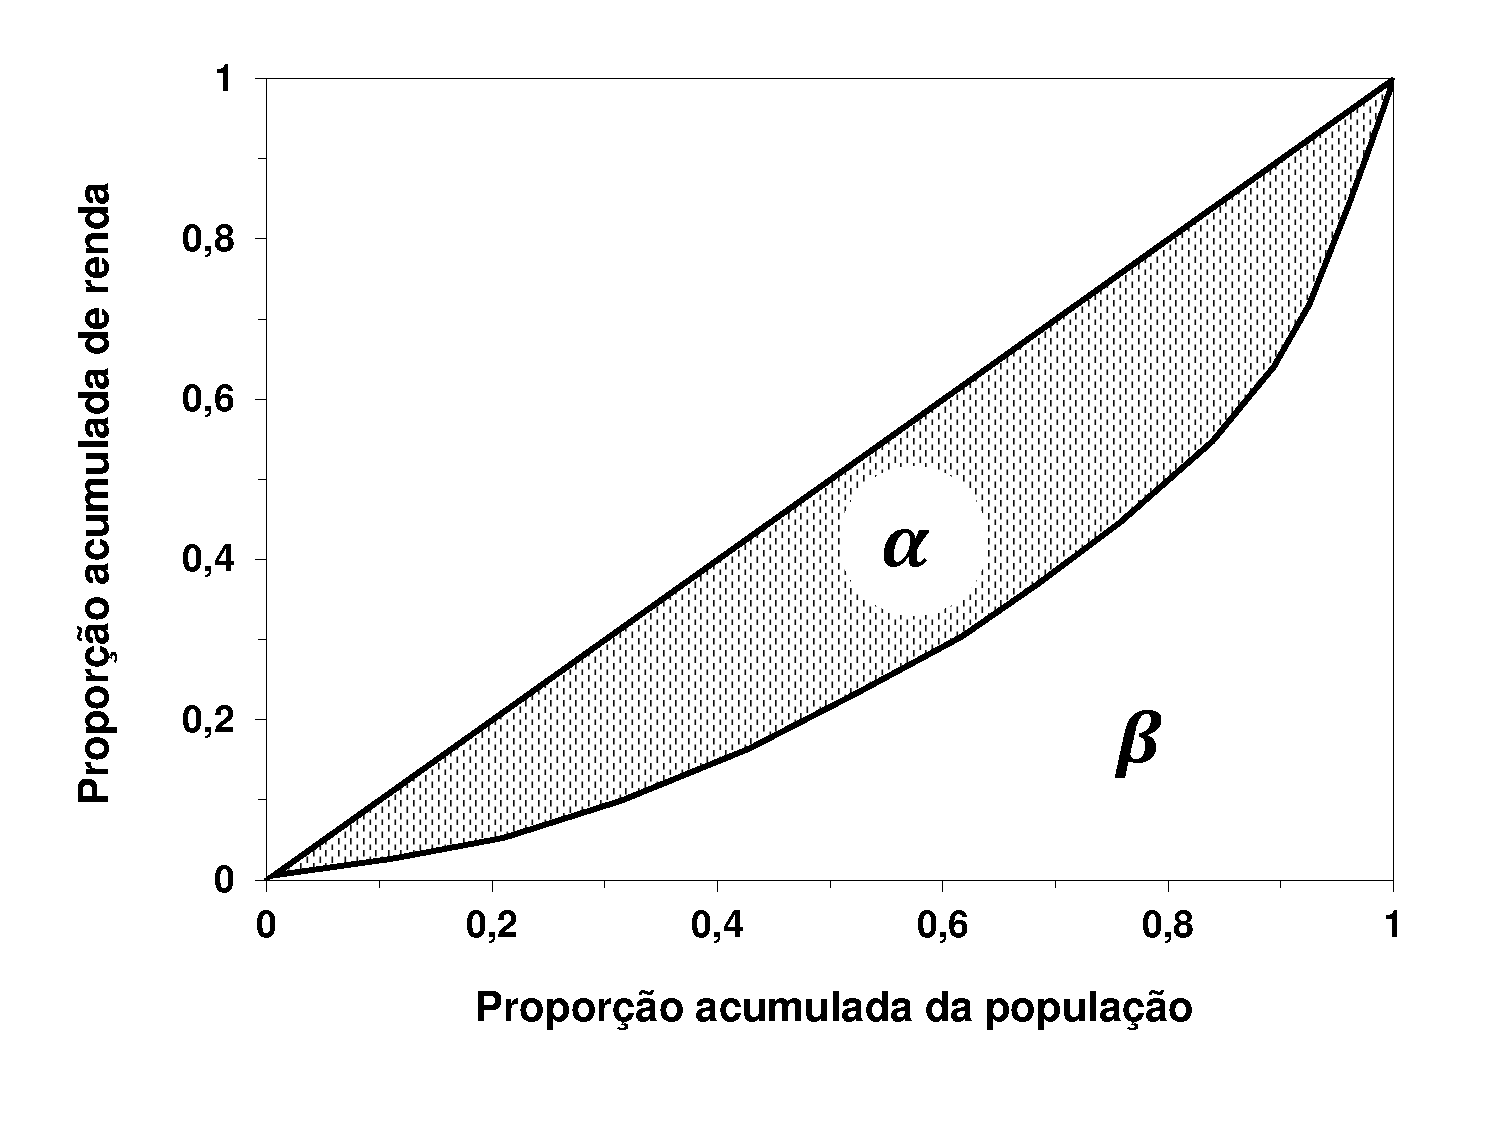
\includegraphics[width=0.8\textwidth]{figs/cap02_curva_lorenz.pdf}
   \caption*{\footnotesize{Fonte: Adaptado de \cite{cap02_ref20}}}
   \label{fig:lorenz_curve}
\end{figure}

O coeficiente de Gini corresponde ao quociente da área $\alpha$ com a soma das áreas $\beta$ e $\alpha$, ou seja: 

\begin{equation}
    G = \frac{\alpha}{\alpha + \beta} = \frac{\alpha}{0,5}
    \label{eq:2.5}
\end{equation}

Dessa forma pode-se reescrever a equação~\ref{eq:2.5} como:

\begin{equation}
    G = 1 - 2\beta
    \label{eq:2.6}
\end{equation}

Similarmente, é possível considerar que a renda $x_i$ é composta por $k$ parcelas de rendimento de forma que: 

\begin{equation}
    x_i = \sum_{h=1}^{k}x_{hi}
\end{equation}

\noindent onde $x_{hi}$ representa o valor da $h$-ésima parcela de renda da $i$-ésima pessoa. Sendo assim, a média da $h$-ésima parcela é:

\begin{equation}
    \mu_h = \frac{1}{n} \sum_{i=1}^{n}x_{hi}
\end{equation}

\noindent e a proporção acumulada dessa parcela referente a série~\ref{eq:2.1} é dado por:

\begin{equation}
    \varphi_{hi} = \frac{1}{n\mu_h} \sum_{j=1}^{i} x_{hj}
\end{equation}

Analogamente a equação~\ref{eq:2.6} é possível definir a curva de concentração como sendo a relação dos pares ordenados de $\varphi_{hi}$ e $p_i$. Ressalta-se que na construção da curva de concentração de $x_{hi}$ é utilizada a ordenação de $x_i$ e não a ordenação de $x_{hi}$, que pode ser diferente. Sendo assim, do mesmo modo que para o coeficiente de Gini, define-se a Razão de Concentração da parcela $h$ $(C_h)$ como:

\begin{equation}
	C_h = 1 - 2\beta_h
	\label{eq:2.10}
\end{equation}

\noindent onde $\beta_h$ é a área entre a curva de concentração de $x_{hi}$ e o eixo das abscissas.

Diante disso, \cite{cap02_ref22} demonstra que o índice de Gini é definido pela média ponderada das razões de concentração das parcelas $h$. Então:

\begin{equation}
	G = \sum_{h=1}^{k} \varphi_h C_h
\end{equation}

\noindent como $\sum_{h=1}^{} \varphi_h = 1$, pode-se reescrever a equação 1 como:

\begin{equation}
	G = G - \sum_{h=1}^{k} \varphi_h (G - C_h)
\end{equation}

\noindent com, 

\begin{equation}
	\pi_h = G - C_h
	\label{eq:2.13}
\end{equation}

A equação~\ref{eq:2.13} é conhecida como medida de progressividade, na qual $\pi_h > 0$ ($C_h < G$) simboliza uma parcela progressiva (contribuindo para o decréscimo do índice de Gini e diminuição da concentração de renda). De forma semelhante $\pi_h < 0$ ($C_h > G$) corresponde a uma parcela regressiva (contribuindo para o acréscimo do índice de Gini e aumentando a concentração de renda) \cite{cap02_ref22}.

\subsection{Correlação de Variáveis}\label{cap:referencias:correlacao}

Em estatística, correlação compreender a interdependência existente entre duas variáveis, ou seja, o grau de relacionamento ou associação existentes entre as características de um dado. Em alguns casos essa relação é clara, como a massa corporal e a altura de uma pessoa, o consumo de combustível e a distância percorrida por um veículo ou o número de anúncios divulgados e a quantidade de produtos vendidos. Todavia, em muitos casos essa interdependência não é intuitiva ou aparente, fazendo necessário, dessa forma, a utilização de estratégias matemáticas para aferir essa correlação \cite{cap02_ref39}. Dentre os métodos mais comuns temos os índices de Pearson, Spearman e Kendall.

O coeficiente de correlação de Pearson, também conhecido como coeficiente de correlação produto-momento, é responsável por mensurar a interdependência, positiva ou negativa, existente entre duas variáveis. Essa estimativa, normalmente representada por $\rho$, assume valores entre -1 e 1, onde 1 corresponde a uma correlação perfeita positiva entre as variáveis, e -1 a uma correlação perfeita negativa, ou seja, se uma aumenta a outra sempre diminui. Por outro lado, quando o valor de $\rho$ é igual 0 observa-se uma interdependência linear entre as variáveis, podendo, no entanto, existir uma dependência não-linear entre elas \cite{cap02_ref41, cap02_ref40}.

O cálculo do coeficiente de correlação de Pearson pode ser realizado a partir da seguinte fórmula: 

\begin{equation}
    \rho = \frac{cov(X,Y)}{\sqrt{var(X).var(Y)}} = \frac{\sum_{i=1}^{n} (x_{i} - \bar{x})(y_{i} - \bar{y})} {\sqrt{\sum_{i=1}^{n} (x_{i} - \bar{x})^2} . \sqrt{\sum_{i=1}^{n} (y_{i} - \bar{y})^2}}
    \label{eq:2.14}
\end{equation}

\noindent onde, $x_{1}, x_{2}, ..., x_{n}$ e $y_{1}, y_{2}, ..., y_{n}$ correspondem aos valores assumidos por cada variável, e $\bar{x}$ e $\bar{y}$ são suas respectivas médias aritméticas.

A correlação de Pearson mensura a associação linear entre variáveis contínuas, estimando o quanto a relação dessas variáveis pode ser descrita por uma reta \cite{cap02_ref41}. Diante disso, pode ser interpretar o valor de $\rho$ como:

\begin{itemize}
    \item 0,9 a 1 positivo ou negativo indica uma correlação muito forte.
    \item 0.7 a 0.9 positivo ou negativo indica uma correlação forte.
    \item 0.5 a 0.7 positivo ou negativo indica uma correlação moderada.
    \item 0.3 a 0.5 positivo ou negativo indica uma correlação fraca.
    \item 0 a 0.3 positivo ou negativo indica uma correlação desprezível.
\end{itemize}

De maneira similar, o coeficiente de Spearman é comumente utilizado para aferir a interdependência existente entre variáveis aleatórias relacionadas monotonicamente\footnote{Uma função entre dois conjuntos de dados é considerada monótona quando há a preservação da relação de ordem no seu domínio.}, mas não de maneira linear. A forma deste coeficiente de correlação é a mesma do coeficiente de Pearson, mas as variáveis não correspondem mais aos valores originais coletados, substituindo-os por postos correspondes ao valor que cada variável assume em uma ordenação numérica \cite{cap02_ref39}.

O coeficiente de correlação de Spearman pode ser aferido da seguinte forma: 

\begin{equation}
    \rho = 1 - \frac{6 \ \mathlarger{\sum_{i-1}^{n}} \ (X - Y)^2}{n(n^2 - 1)}
    \label{eq:2.15}
\end{equation}

\noindent onde $X$ e $Y$ são as variáveis aleatórias variando de 1 a $n$, com $n$ sendo a quantidade de elementos existentes no conjunto.

O coeficiente de Kendall, por sua vez, avalia a interdependência de postos ordenados, semelhante a correlação de Spearman. Essa medida é comumente eficiente para dados discretos, na qual $\left(x_1, y_1\right)$, $\left(x_2, y_2\right)$, ..., $\left(x_n, y_n\right)$ compreendem conjuntos de observações das variáveis aleatórias $X$ e $Y$, tal que $x_i$ e $y_i$ sejam valores únicos. Qualquer par ordenado de observações, em que $i\ \neq\ j$, é considerado concordante se as classificações dos elementos concordarem entre si, ou seja, se $x_i > x_j$ e $y_i > y_j$, ou se $x_i < x_j$ e $y_i < y_j$. De maneira similar, eles serão discordantes se $x_i > x_j$ e $y_i < y_j$, ou se $x_i > x_j$ e $y_i < y_j$. Na hipótese de $x_i = x_j$ e $y_i = y_j$, o par não será nem concordante e nem discordante \cite{cap02_ref42, cap02_ref39}. Dessa forma, é possível calcular o coeficiente de correlação de Kendall $(\tau)$ conforme a Equação~\ref{eq:2.16}:

\begin{equation}
    \tau = \frac{(quantidade \ de \ pares \ concordantes) - (quantidade \ de \ pares \ discordantes)}{n(n - 1)/2}
    \label{eq:2.16}
\end{equation}

É importante destacar que a correlação não indica necessariamente causa. Por exemplo, considere um estudante que teve boas notas nas disciplinas de química e física. O bom desempenho em química não pode ser necessariamente atribuído ao bom desempenho em física, mas ambas as notas podem ser explicas por um bom desempenho em matemática, fator não considerado no primeiro momento. Dessa forma, a correlação apresenta-se como uma importante ferramenta para análise de dados uma vez que, quando interpretada corretamente, possibilita a abstração de informações relevantes acerca de conjuntos de atributos interdependentes.

% --------------------------------------------------------------------------- %
\section{Considerações Finais}

Nesse capítulo foi apresentada a fundamentação teórica que norteou o desenvolvimento desta dissertação, iniciando por uma contextualização acerca de análise de dados, a qual evidenciou o conceito de processo de extração de conhecimento \cite{cap02_ref12} – relatando a sua diferença em relação a mineração de dados \cite{cap02_ref5} – e suas aplicações no cenário empresarial a partir do método de BI \cite{cap02_ref15, cap02_ref16}. Com base nessas definições, foi realizada a conceituação de ciência de dados \cite{cap02_ref9, cap02_ref1, cap02_ref3}, relatando sua relevância perante o atual cenário de produção de informações \cite{cap02_ref4} e evidenciando sua capacidade adaptativa de trafegar entre as diversas áreas de conhecimento \cite{cap02_ref2}.

Posteriormente, foi apresentado o conceito de dados abertos destacando sua importância nos mais diversos campos como ferramenta de acesso a informação para a sociedade \cite{cap02_ref4}. Nesse âmbito, enfatizou-se os dados abertos governamentais como mecanismo para a disponibilização de conteúdo público para a população, objetivando oferecer um sistema governamental mais transparente tanto no Brasil como em diversos países do mundo \cite{cap02_ref25}.

Por fim, foram conceituadas algumas das técnicas matemáticas utilizadas nesta pesquisa. Primeiramente, fez-se uma definição acerca da decomposição do coeficiente de Gini \cite{cap02_ref19}, destacando sua utilização para aferir o grau de desigualdade de uma população acerca de uma determinada variável, como por exemplo a seu rendimentom e sua capacidade de mensurar o quanto cada parcela dessa variável influencia para diminuir ou aumentar a desigualdade existente. Em seguida, foram detalhados os conceitos de correlação entre variáveis interdependes, enfatizando sua eficiência para abstração de informação útil acerca de atributos em conjuntos de dados \cite{cap02_ref39}.


\chapter{Trabalhos Correlatos}\label{cap:estArte}

\section{Considerações Iniciais}\label{sec:primTrab}

O processo de extração de conhecimento válido acerca de bases de dados abertas públicas, seja pela ótica da ciência de dados ou análise de dados tradicional, apresenta-se como uma importante linha de pesquisa tanto na área da computação aplicada quanto nos demais campos interdisciplinares. Com isso, diversos trabalhos referentes a essa temática objetivam, de forma geral, compreender aspectos econômicos e sociais ou propostas governamentais baseando-se em simulações de cenários, análises estatísticas, aplicação de modelos de inteligência computacional e observações críticas acerca dos resultados, utilizando como objeto de estudos os dados relacionados a problemática abordada. 

Diante disso, o presente capítulo apresenta um panorama geral dos estudos correlacionados a temática abordada nessa dissertação, explicitando os trabalhos julgados mais relevantes perante a problemática descrita no escopo desta pesquisa. Dessa forma, a Tabela~\ref{tab:cap03:correlatos} apresenta uma síntese acerca desses trabalhos correlatos, mostrando de maneira concisa as considerações realizadas acerca dos mesmos. 


\section{Correlatos}

A aplicação da ciência ou análise de dados em dados abertos públicos apresenta-se promissora, e difusa, em meio aos diversos segmentos governamentais. Estudos utilizando os microdados da economia, educação e saúde pública, por exemplo, tendem a apresentar informações relevantes para a compreensão de alguns fenômenos sociais e podem servir como subsídio para auxiliar tomadas de decisões em gestão pública \cite{cap03_ref1, cap03_ref2}. Avaliando o estado da arte da previdência social brasileira, eixo temático desta pesquisa, evidenciam-se, no geral, trabalhos que objetivam compreender e discutir a sua contribuição social e a transparência dos modelos propostos pelo governo relativos à sustentabilidade do sistema.

Dessa forma, acerca dos impactos socioeconômicos causados pela previdência social nacional, o trabalho de \cite{cap02_ref22} utilizou dados da PNAD de 2001 a 2007 para verificar quais variáveis de rendimento influenciam na redução ou aumento da desigualdade de distribuição renda – mensurada através da decomposição do índice de Gini, semelhante ao demonstrado na subseção~\ref{cap:referencias:gini} desta dissertação. Os resultados demonstraram que a parcela de aposentadorias e pensões, embora tenham colaborado para a redução do coeficiente de Gini com alterações ocorridas no decorrer dos anos, apresentava regressividade, ou seja, colaboram para um aumento na concentração de renda. Além disso, destaca-se que embora o trabalho não seja recente, o mesmo apresentou importantes discussões que colaboraram para um melhor compreendimento da problemática abordada nessa pesquisa.

O trabalho de \cite{cap04_ref11}, semelhante ao anterior, avalia a participação que os benefícios de aposentadorias e pensões, oficiais e não oficiais, apresentam na desigualdade de rendimento dos domicílios brasileiros. A autora utiliza os dados da Pesquisa Nacional por Amostra de Domicílios (PNAD) de 2004 a 2017 e a metodologia de decomposição do índice de Gini, aplicando-os no Brasil e suas regiões, semelhante ao trabalho anterior. No entanto, seus resultados demonstraram que esses benefícios apresentam características diferentes quando divididos em categorias de salários, ou seja, as aposentadorias e pensões até um salário mínimo colaboram para a desconcentração de renda, enquanto as acima de um salário mínimo apresentavam característica oposta, contribuindo para aumentar o coeficiente de Gini. 

Em \cite{cap03_ref3} foram utilizados os dados censitários, disponibilizados pelo Instituto Paranaense de Desenvolvimento Econômico e Social (IPARDES), dos anos de 1980, 1991, 2000 e 2010 para os 399 municípios paranaenses, e microdados de rendimento presentes nas PNADs de 1988 a 2012, objetivando compreender o processo de envelhecimento da população no estado e seus impactos socioeconômicos na distribuição de renda da população. O estudo demonstrou que no intervalo de 30 anos avaliado, a proporção de pessoas acima de 60 anos mais que triplicou, provocando um aumento paralelo no percentual de participação dos benefícios de aposentadorias e pensões na renda total, apontando, dessa forma, uma preocupação na formação de políticas públicas ao mercado de trabalho, sistema de previdência, saúde e lazer para o público analisado.

A pesquisa de \cite{cap03_ref4}, por sua vez, propôs um modelo econométrico para compreender como a previdência social atua sobre as distribuições de renda regionais e estaduais no Brasil. Os resultados demonstraram que, em 2010, o sistema previdenciário foi um instrumento eficaz para a melhoria na distribuição de renda regional, mensurada através do índice de Gini, a qual apresentou impactos positivos diretos no PIB per capita brasileiro. 

Em \cite{cap04_ref12} foram utilizados dados municipais relacionados a pagamentos de benefícios de aposentadorias, arrecadações e fundo de participação municipal, de 2017, para compreender o cenário previdenciário nacional. Mediante a isso, o estudo destaca a Previdência Social como principal instrumento assistencial para o combate à pobreza, relatando que, sem os benefícios pagos mensalmente aos pensionistas e aposentados, diversas áreas rurais dos municípios de pequeno porte estariam em situação de calamidade social.

Por outro lado, a literatura apresenta diversos trabalhos relacionados à sustentabilidade do sistema previdenciário brasileiro e à transparência das políticas públicas que tangenciam essa temática. Com isso, o trabalho de  \cite{cap03_ref5}, por exemplo, buscou quantificar, usando um modelo de previsão a longo prazo, o impacto da demografia sobre as despesas da previdência social como proporção do Produto interno Bruto (PIB) para o Brasil. A pesquisa utilizou um modelo simples de projeção, demostrando que em 2060 as despesas do sistema compreenderiam aproximadamente 19\% do PIB nacional. Entretanto, apesar da grande relevância dos resultados, o modelo é útil apenas para ilustrar os efeitos do envelhecimento da população em relação às despesas previdenciárias, não sendo apropriado para investigações acerca de propostas de reforma. 

Em \cite{cap05_ref9}, os autores, motivados pelas discussões políticas acerca da reforma da previdência prevista na PEC 287/16, investigaram os resultados divulgados pelo governo federal, os quais foram utilizados para justificar a proposta de política pública. O trabalho apontou que os dados oficiais apresentavam projeções tendenciosas a curto prazo e com erros elevados a longo prazo, uma vez que tais estimativas não consideravam intervalos de confiança. Além disso, a pesquisa relatou a impossibilidade de reprodução dos resultados divulgados pela Lei de Diretrizes Orçamentarias (LDOs), devido, principalmente, à falta de transparência nesses documentos oficiais, tanto na sua metodologia quanto nos dados utilizados.

A pesquisa de \cite{cap03_ref6} apresenta um panorama detalhado referente a atual situação da Previdência Social brasileira, elencando os principais pontos previstos pela PEC 287/16 e relatando os fatores econômicos utilizados para justifica-la. Os autores classificam a proposta citada como imprescindível para a garantia da sustentabilidade fiscal do país, uma vez que o acelerado envelhecimento populacional eleva os custos excessivos de financiamento para as gerações futuras. Semelhantemente, o trabalho de \cite{cap03_ref7} afirma que na ausência de uma reforma, será praticamente impossível respeitar o teto do gasto público até o ano de 2026, último ano de vigência antes de uma possível revisão. Diante disso, o estudo discute a PEC 287/16 e outras duas reformas, sendo uma elaborada pelos autores, demonstrando que, caso aprovado, um reajuste nas diretrizes do sistema previdenciário possibilitaria um controle no teto de gastos, proporcionando condições para a continuidade e crescimento do programa.

Por outro lado, em \cite{cap05_ref10} foram identificadas falsificações, ou possíveis erros, nos resultados utilizados pelo governo federal para justificar a reforma previdenciária PEC 06/2019. Utilizando as planilhas oficiais do Ministério da Economia referentes a Reforma da Previdência, obtidas através da LAI, foram refeitos os cálculos, demonstrando que os benefícios de aposentadorias dos trabalhadores mais pobre diminuem com a reforma proposta. Além disso, notou-se que as aposentadorias obtidas por tempo de contribuição – principal alvo da reforma –, pelas regras atuais, com idades mais novas, financiam os benefícios de menor valor dos trabalhadores que se aposentam com idade mais avançada, fator que, possivelmente, colabora para redução da desigualdade social.

É importante destacar que, embora tenham participação direta na construção desta dissertação, nenhum dos trabalhos citados acima investigou a participação que as aposentadorias e pensões têm na distribuição de renda municipal do Brasil, e nem os efeitos que a uma reforma previdenciária causaria na concessão desses benefícios, principais objetivos desta dissertação. Dessa forma, objetivando esclarecer de forma resumida a abordagem de cada pesquisa, a Tabela~\ref{tab:cap03:correlatos} apresenta uma síntese dos trabalhos correlatos a esta pesquisa ressaltando as principais lacunas identificadas.

\begin{longtable}{|p{0.25\textwidth}|p{0.35\textwidth}|p{0.35\textwidth}|}
\caption{Síntese dos principais trabalhos correlatos.}
\\\hline 
\textbf{Referência} & \textbf{Objetivos} & \textbf{Lacunas} \\ \hline
\footnotesize{(HOFFMANN, 2009)} & Avaliar o impacto que as aposentadorias e pensões causam na distribuição de renda do Brasil entre 2001 e 2007 & Concentra-se em uma avaliação nacional, não abordando unidades territoriais menores \\ \hline
\footnotesize{(NAKATANI-MACEDO, 2015)} & Avaliar o impacto que as aposentadorias e pensões causam na distribuição de renda do Brasil e regiões entre 2004 e 2014 & Concentra-se em uma avaliação nacional e estadual, não abordando unidades territoriais menores \\ \hline
\footnotesize{(NAKATANI-MACEDO et al., 2015)} & Avaliar o impacto que as aposentadorias e pensões causam na distribuição de renda do estado do Paraná e regiões entre 1980 e 2010 & Concentra-se em uma avaliação isolada de apenas um estado brasileiro \\ \hline
\footnotesize{(BARBOSA, 2015)} & Propor um modelo econométrico que compreenda como as aposentadorias implicam na distribuição de renda das regiões e estados brasileiros & Semelhante aos anteriores, não aplica uma avaliação acerca de unidades territoriais menores \\ \hline
\footnotesize{(SOLÓN, 2019)} & Utiliza dados previdenciários municipais de 2017 para avaliar a situação do sistema em cada cidade & Não estima o impacto que os benefícios causam na distribuição de renda da população de cada município \\ \hline
\footnotesize{(COSTANZI; ANSILIERO, 2017)} & Aplica um modelo de previsão a longo prazo para avaliar a a situação da Previdência Social em 2060 & Não considera os impactos sociais que uma reforma provocaria e suas projeções não apresentam intervalos de confiança \\ \hline
\footnotesize{(SILVA et al., 2017)} & Recalcular as projeção realizadas pelo governo para verificar se os argumentos utilizadas para justificar  a PEC 287/16 eram válidos & Não avaliou os possíveis impactos sociais que reforma a reforma proposta causaria \\ \hline
\footnotesize{(COSTANZI et al., 2018)} & Elencar os principais pontos da PEC 287/16 mediante a atual situação do sistema previdenciário nacional & Não pondera os possíveis pontos negativos que a proposta acarretaria no cenário social dos trabalhadores \\ \hline
\footnotesize{(GIAMBIAGI;PINTO; ROTHMULLER, 2018)} & Avaliar a PEC 287/16, e outras duas reformas, como alternativas para controlar os gastos públicos do sistema previdenciário nacional & Semelhante ao anterior, desconsidera os impactos sociais que as propostas poderiam causar \\ \hline
\footnotesize{(BASTOS et al., 2019)} & Recalcular os resultados divulgados pelo governo utilizados para justificar a reforma da previdência correspondente a PEC 06/2019 & O estudo, embora enfatize os aspectos sociais negativos da reforma, não apresenta estimativas acerca do cenário previdenciário \\ \hline
%\end{tabular}
\caption*{\footnotesize{Elaborado pelo autor.}}
\label{tab:cap03:correlatos}
\end{longtable}

\section{Considerações Finais}
Este capítulo apresentou os trabalhos correlatos que nortearam a realização dessa pesquisa. Avaliando o estado da arte da problemática abordada nessa dissertação, observa-se um conjunto de estudos referente à análise dos impactos socioeconômicos gerados pelo sistema previdenciário brasileiro, e à avaliação da sustentabilidade de propostas governamentais. Todavia, destaca-se que grande parte desses estudos não aborda nas suas metodologias as aplicações de técnicas, ou estratégias, de análise de dados, normalmente utilizadas para a abstração dos resultados discutidos.

Nesse contexto, os estudos de caso propostos por essa pesquisa realizam uma abordagem diferente da comumente encontrada na literatura. Além da avaliação crítica realizada acerca das análises propostas, será detalhado o procedimento metodológico utilizado - desde a extração dos dados sem representatividade, até a abstração de conhecimento válido acerca dos resultados gerados. Tal abordagem apresenta-se promissora, dentre outros fatores, por possibilitar a replicação do trabalho pela comunidade científica, proporcionando, dessa forma, o desenvolvimento de uma pesquisa colaborativa mais eficiente.



\chapter{Análise da Participação das Aposentadorias e Pensões na Distribuição de Renda do Brasil, 2000 e 2010}

% --------------------------------------------------------------------------- %
\section{Considerações Iniciais}

A distribuição de renda, ou distribuição de riquezas, de um país é um tópico de inquestionável importância em todos os seguimentos da sociedade devido, principalmente, ao fato de estar diretamente relacionado com as condições de vida da população. Tal assunto apresenta-se em constante evidencia no cenário brasileiro uma vez que esse apresenta-se como um dos países mais desiguais do mundo \cite{cap04_ref2, cap04_ref3}. De acordo com dados da \cite{cap04_ref1}, o Brasil ocupa a 156ª posição\footnote{Não há dados atualizados de índice de Gini em diversos países, indicando dessa forma que, possivelmente, o Brasil não ocupe exatamente a posição informada.}  no ranking de índices de Gini de mundo, corroborando para que grande parte da população nacional tenha rendimentos insuficientes para atender suas necessidades básicas.

Entretanto, informações anuais divulgadas pela PNAD revelam que a desigualdade de renda nacional sofreu uma substancial redução nos últimos anos \cite{cap04_ref4} - ainda que se apresente muito elevada comparada a outros países do mundo. Paralelamente a esse fator, outros indicadores do mercado de trabalho, como taxas de informalidade e desemprego, demonstram-se regressivos nos últimos anos, apontando possível contribuição para a diminuição do índice de Gini registrada. A Figura~\ref{fig:cap04:gini_taxas} ilustra o comportamento dessas métricas no Brasil entre os anos de 2001-2014.

\begin{figure}[!h]
    \centering
    \caption{Variação das taxas de formalidade e fesemprego e do índice de Gini no Brasil, 2001 a 2014}
    \includegraphics[width=0.8\textwidth]{figs/cap04_gini_taxas.pdf}
    \caption*{\footnotesize{Fonte: Elaborado pelo autor a partir de dados contidos em  \cite{cap04_ref4}}}
    \label{fig:cap04:gini_taxas}
\end{figure}

Paralelamente, os benefícios de aposentadorias e pensões compreendem uma importante parcela de rendimento da população, apresentando-se cada vez mais ativos na composição de renda dos domicílios brasileiros \cite{cap02_ref22, cap04_ref5}. Esses benefícios, em sua grande maioria, correspondem a repasses garantidos pela Previdência Social, objetivando assegurar o rendimento dos contribuintes quando esses não detêm mais de suas capacidades laborais \cite{cap04_ref6}.

Diante desse fator, oberava-se na literatura uma divergência de pontos de vista relacionados a contribuição dessa parcela de benefícios para o aumento ou diminuição da distribuição de renda no Brasil. Alguns trabalhos como \cite{cap04_ref7, cap04_ref8, cap04_ref9} indicam que as aposentadorias e pensões colaboram para o crescimento do coeficiente de Gini tanto em escala nacional quanto regional. No entanto, as pesquisas de \cite{cap04_ref10, cap04_ref11} demonstram que essa parcela de benefícios colabora para a redução da desigualdade de renda no Brasil.

Revisando o estado da arte relacionado a essa problemática, nota-se que grande parte dos estudos abstraem seus \textit{insights} a partir dos microdados anuais divulgados pela PNAD. Entretanto, tal estratégia restringe as possibilidades de avaliações a serem realizadas em virtude dessa pesquisa corresponder a uma amostra domiciliar efetuada nas unidades federativas brasileiras, impossibilitando a flexibilidade para análises em unidades territoriais menores como municípios ou setores censitários. Uma avaliação municipal da proporcionalidade entre a distribuição de renda e os repasses de aposentadorias e pensões, apresenta-se como uma importante forma de compreender o real impacto que esses benefícios causam no coeficiente de Gini nacional. Tal importância destaca-se no trabalho de \cite{cap04_ref12}, o qual compreende a previdência social como instrumento assistencial que combate à pobreza em diversos municípios brasileiros.

Diante disso, neste estudo de caso é realizada uma avaliação da participação que os rendimentos de aposentadorias e pensões tem na distribuição de riquezas dos estados e municípios do Brasil. Para tanto, optou-se por utilizar estratégias e conceitos de ciência de dados acerca dos microdados dos censos demográficos de 2000 e 2010, e a metodologia de decomposição do índice de Gini - conforme descrito no capítulo ~\ref{cap:referencias} - para aferir o grau de contribuição das parcelas desejadas.

Dessa forma, esse capítulo foi dividido em 4 subseções incluindo esta introdução. Na subseção~\ref{cap04:metodologia}, será abordada a metodologia utilizada para o desenvolvimento das análises propostas, demonstrando detalhadamente os tratamentos e processamentos efetuados acerca dos dados. Na subseção~\ref{cap04:resultados} serão discutidos os principais resultados encontrados, finalizando o estudo na subseção~\ref{cap04:conclusoes} com as considerações finais. 

\section{Metodologia Utilizada}\label{cap04:metodologia}

O procedimento metodológico para a realização do estudo proposto foi sistematizado mediante a uma sequência de etapas de análise de dados: extração, pré-processamento, aplicação de modelos matemáticos/computacionais e abstração de informações acerca dos dados de entrada. A Figura~\ref{fig:cap04:metodologia} ilustra o fluxograma de desenvolvimento do trabalho contendo cada uma das etapas realizadas, havendo um maior grau de detalhamentos acerca destas no decorrer dessa subseção. 

\begin{figure}[!h]
    \centering
    \caption{Fluxograma de desenvolvimento do primeiro estudo de caso}
    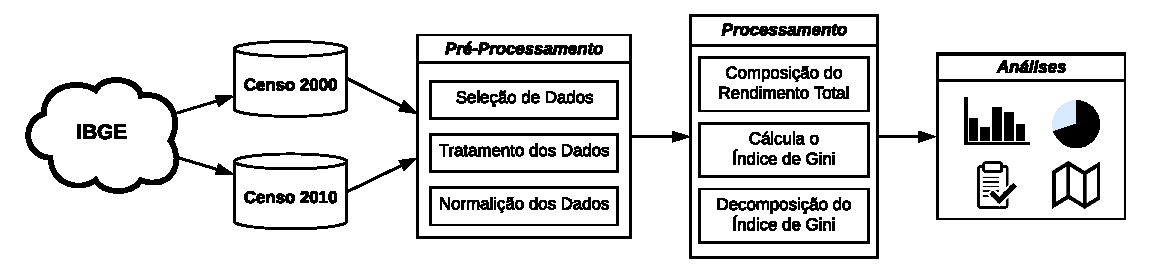
\includegraphics[width=\textwidth]{figs/cap04_metodologia_estudo01.pdf}
    \caption*{\footnotesize{Fonte: Elaborado pelo autor}}
    \label{fig:cap04:metodologia}
\end{figure}

% --------------------------------------------------------------------------- %

\subsection{Origem dos Dados}

Os microdados utilizados na execução das análises desse estudo foram extraídos dos censos demográficos realizados pelo IBGE nos anos de 2000 e 2010. As informações referentes aos censos anteriores, como por exemplo 1991, foram desconsiderados na pesquisa devido aos altos índices de inflação recorrentes na época \cite{cap04_ref13}, gerando por consequência baixa confiabilidade nos resultados gerados.

O censo demográfico brasileiro trata-se de uma pesquisa nacional realizada cada dez anos, visando o reconhecimento das condições de vida da população brasileira em todas as grandes regiões, unidades federativas, mesorregiões, microrregiões, regiões metropolitanas, municípios, distritos, subdistritos e setores censitários, tendo como objeto de coleta as pessoas residentes (na data de referência) em domicílios presentes no território nacional \cite{cap04_ref14}. No site do censo\footnote{Disponível em: <https://www.ibge.gov.br/estatisticas/sociais/populacao/9662-censo-demografico> Acesso em: 20 Dez, 2019} é possível encontrar os principais resultados, estatísticas, tabelas e publicações realizadas pelo IBGE. Entretanto, o instituto também fornece os microdados e documentação referentes a cada pesquisa realizada, possibilitando que a comunidade acadêmica, empresas ou até mesmo pessoas físicas realizem pesquisas acerca destes. 

Os microdados disponibilizados pelas bases são divididos em 3 grupos de informações, os quais abrangem pessoas, famílias e domicílios. Essa classificação possibilita estudos estatísticos acerca de qualquer uma dessas categorias de forma isolada, permitindo análises com alto grau de detalhamento, dependendo da dimensão da problemática em questão. O presente trabalho norteou-se a partir das classes pessoas e domicílios, com recortes espaciais para as unidades federativas e municípios brasileiros. 

O censo demográfico difere-se da PNAD, principalmente, em abrangência territorial e quantidade de informações exploradas. Enquanto a primeira pesquisa realiza uma investigação profunda em todo território nacional sobre as características socioeconômicas\footnote{Resumidamente, o censo demográfico aborda os seguintes temas: características dos domicílios, identificação étnico-racial, nupcialidade, núcleo familiar, religião, deficiência, migração, educação, trabalho, rendimento e mortalidade.} da população, a segunda propõe uma apuração domiciliar mais limitada\footnote{Os temas abordados na PNAD são: habitação, características gerais dos moradores, características do trabalho, rendimentos e educação.}, restringindo apenas ao grau de representatividade necessária para os seus resultados acerca dos diversos níveis geográficos\footnote{A PNAD abrange o Brasil, Grandes Regiões, Unidades da Federação, Regiões Metropolitanas que contêm Municípios das Capitais, Municípios das Capitais e Região Integrada de Desenvolvimento da Grande Teresina.} definidos na sua divulgação.

\subsection{Pré-Processamento dos Dados}

Os censos demográficos foram carregados em um Sistema Gerenciador de Banco de Dados (SGBD) objetivando facilitar as consultas acerca dos microdados em questão. Constatou-se que a base de dados do ano 2000 possuía mais de 280 variáveis relacionadas à domicílios, famílias e pessoas, e que a de 2010 ultrapassava 350 variáveis correspondentes a domicílios, pessoas, mortalidade e emigração. Dessa forma, foi realizada uma etapa preliminar de seleção de atributos com o intuito de filtrar somente as informações de interesse para as posteriores análises. A Tabela~\ref{tab:cap04:variaveis} exibe as 7 variáveis utilizadas no presente estudo e suas respectivas descrições.
	
\begin{table}[!h]
    \centering
    \caption{Variáveis selecionadas dos censos demográficos e suas descrições} 
    \begin{tabular}{|p{2cm}|p{2cm}|p{10cm}|}
        \hline
        \multicolumn{2}{|c|}{\textbf{Código das Variáveis}} & \multicolumn{1}{c|}{\multirow{2}{*}{\textbf{Descrição}}} \\ \cline{1-2}
        \centering\textbf{2000} & \centering\textbf{2010} & \multicolumn{1}{c|}{} \\ \hline
        \centering v0102 & \centering v0001 & Código do estado \\ \hline
        \centering v0103 & \centering v0002 & Código do município \\ \hline
        \centering v7616 & \centering v6529 & Rendimento mensal domiciliar \\ \hline 
        \centering v4614 & \centering v6527 & Rendimento mensal per capita \\ \hline
        \centering v4573 & \centering v6591 & Rendimento dos benefícios de aposentadorias e pensões \\ \hline
        \centering - & \centering v0656 & Aposentadorias e pensões da Previdência Social \\ \hline
        \centering p001 & \centering v0010 & Peso de cada registro\\ \hline
    \end{tabular}
    \caption*{\footnotesize{Fonte: Elaborado pelo autor a partir dos metadados dos censos demográficos de 2000 e 2010}}
    \label{tab:cap04:variaveis}
\end{table}

A seleção dessas variáveis norteou-se com base nas informações necessárias para mensurar o grau de desigualdade e calcular a decomposição do índice de Gini (conforme demonstrado na subseção~\ref{cap:referencias:gini}) acerca das unidades territoriais de interesse.  Observando a Tabela~\ref{tab:cap04:variaveis}, nota-se a presença de um atributo extra na base do censo demográfico do ano de 2010, tal fator é explicado pela necessidade de uma variável auxiliar para designar a qual programa social cada benefício pertence. Adicionalmente foram utilizados os valores de salário mínimo registrados nos meses de abril de ambos os anos abordados, sendo 151 e 510 reais para 2000 e 2010 respectivamente.

Posteriormente, foi realizada uma etapa de tratamento de dados objetivando corrigir erros e possíveis inconsistências existentes nas bases. Devido ao fato de ser uma pesquisa com elevado grau de importância e responsabilidade, foram identificadas poucas anomalias que comprometessem as análises realizadas. No entanto, foi necessária a substituição dos dados ausentes de rendimentos de aposentadorias e pensões por valores zeros (casos específicos de pessoas que não gozavam desses benefícios) e a correção dos pesos que apresentavam escalas erradas em estados e cidades especificas. 

Além disso, em decorrência do elevado dinamismo da malha territorial brasileira \cite{cap04_ref17}, constatou-se uma divergência no número de municípios existente em cada base de dados, registrando 5.507 cidades para o ano de 2000 e 5.564 para 2010. Dessa forma, houve a necessidade de normalizar o número de cidades para ambos os anos adotando como estratégia a criação de Área Mínimas Comparáveis (AMC), as quais são definidas como sendo áreas geográficas com a máxima unidade territorial desagregada, possibilitando dessa forma a comparação entre dois pontos diferentes no tempo \cite{cap04_ref15, cap04_ref16}. Sendo assim, define-se cada AMC como:

\begin{equation}
    AMC(p, r, b, w) = \sum_{i}^{n} mun_{i}(p, r, b, w), \{\forall n \in N\}
\end{equation}

\noindent onde, $p$ corresponde à população, $r$ aos rendimentos, $b$ os valores dos benefícios de aposentadorias e pensões e $w$ os pesos de cada município $n$. Sendo $N$ cada subconjunto de municípios que foram desmembrados em relação aos originais do ano 2000.

% --------------------------------------------------------------------------- %

\subsection{Processamento}

Após a realização dos estágios de seleção, tratamento e normalização dos microdados, foi possível efetuar a etapa de processamento, sendo essa responsável por mensurar os valores do coeficiente de Gini, o percentual de participação das aposentadorias e pensões e o impacto que esses benefícios causam na distribuição de renda da população acerca das unidades territoriais de interesse Para isso, foi adotada a metodologia abordada na subseção~\ref{cap:referencias:gini}, utilizando como parâmetros das equações as variáveis contidas na Tabela~\ref{tab:cap04:parametros}.  

\begin{table}[!ht]
    \centering
    \caption{Parâmetros de indexação e notação geral.} 
    \begin{tabular}{|c|c|c|}
        \hline
        Variável & Significado                & Valor                                 \\ \hline
        k        & estado                     & São Paulo, Rio de Janeiro, Pará, etc. \\ \hline
        i        & cidade                     & Fortaleza, Belém, Curitiba, etc.      \\ \hline
        r        & renda per capita           & R\$ 0, ... , R\$ 1.000, ...           \\ \hline
        d        & renda domiciliar           & R\$ 0, ... , R\$ 1.000, ...           \\ \hline
        b        & renda aposentadoria/pensão & R\$ 0, ... , R\$ 1.000, ...           \\ \hline
        s        & salário mínimo             & R\$ 151 ou R\$ 510                    \\ \hline
        t        & ano                        & 2000 ou 2010                          \\ \hline
        p        & peso                       & 0, ... , 0.01, ... , 1.10, ...        \\ \hline
    \end{tabular}
    \caption*{\footnotesize{Fonte: Elaborado pelo autor.}}
    \label{tab:cap04:parametros}
\end{table}

Para o cálculo do índice de Gini optou-se por utilizar a renda per capita domiciliar conforme é retratado na literatura \cite{cap02_ref22, cap04_ref10, cap04_ref11, cap04_ref8, cap04_ref1, cap02_ref2}. Dessa forma, o grau de desigualdade dos estados e municípios brasileiros ($Desigualdade$) pode ser interpretado pela Equação~\ref{eq:4.2}, sendo: 

\begin{equation}\label{eq:4.2}
    Desigualdade(t, k, i) = Gini(t, k, i, d, p), \{\forall d > 0\}
\end{equation}

\noindent onde $Desigualdade$ corresponde ao coeficiente de Gini, dos domicílios com rendimento, para cada município $i$ e estado $k$ nos anos $t$, conforme descrito em \ref{eq:2.6}.

Posteriormente, para mensurar o grau de participação das aposentadorias e pensões na composição de renda da população, calculou-se o quociente entre os valores desses benefícios e o total de rendimentos per capita de cada unidade territorial $k$ e $i$, e ano $t$. Dessa forma, pode-se entender o grau de participação ($PartBeneficio$) como sendo: 

\begin{equation}
    PercBeneficios(t, k, i) = \dfrac{\mathlarger{\sum_{N}} \ b(n, p, t, k, i)}{\mathlarger{\sum_{M}} \ r(m, p, t, k, i)}, \{n \subset N \And m \subset M\}
\end{equation}

\noindent sendo $N$ e $M$ os conjuntos universos de valores de renda de aposentadorias/pensões e rendimentos per capita, respectivamente.

Por fim, aferiu-se o impacto que esses benefícios de aposentadorias e pensões causam acerca da variável $Desigualdade$ utilizando a metodologia de decomposição do índice de Gini para cada cidade $i$ e estado $k$ nos anos $t$, semelhante a equação~\ref{eq:4.2}. Sendo assim, estimou-se a razão concentração ($Concentracao$) desses benefícios como:

\begin{equation}\label{eq:4.4}
    Concentracao (t, k, i) = C_h(t, k, i, b, p), \{\forall b > 0\}
\end{equation}

\noindent onde $C_h$ corresponde a Equação descrita em \ref{eq:2.10}. 

Dessa forma, a medida de progressividade ($\pi$) pode ser compreendida por:

\begin{equation}\label{eq:4.5}
    \pi(t, k, i) = Desigualdade(t, k, i) - Concentracao (t, k, i)
\end{equation}

Paralelamente, utilizando os conceitos das Equações~\ref{eq:4.4} e \ref{eq:4.5}, calculou-se também as medidas de progressividade para os benefícios até 1 salário mínimo e acima de 1 salário mínimo acerca de cada unidade salarial $s$. 

Para a realização dos cálculos propostos, foi utilizada a linguagem de programação \textit{Python 3}\footnote{Disponível em: <https://www.python.org/> Acesso em: 05 Jan, 2020}, devido a sua facilidade para trabalhar com grandes volumes de dados, e as bibliotecas de análise dados \textit{Pandas}\footnote{Disponível em: <https://www.pandas.pydata.org/> Acesso em: 05 Jan, 2020}, \textit{Numpy}\footnote{Disponível em: <https://www.numpy.org/> Acesso em: 05 Jan, 2020} e \textit{Scikit-Learn}\footnote{Disponível em: <https://www.scikit-learn.org/stable/> Acesso em: 05 Jan, 2020}. Além disso, foi utilizado o \textit{software} QGIS 2.18\footnote{Disponível em: <https://www.qgis.org/pt\_BR/site/> Acesso em: 05 Jan, 2020} para a elaboração de mapas temáticos objetivando proporcionar uma melhor visualização acerca dos resultados encontrados. O projeto está disponibilizado na plataforma do GitHub\footnote{Disponível em: <https://github.com/jralbbuquerque/censo-beneficio> Acesso em: 05 Jan, 2020} sob uma licença GNU \textit{General Public License} (GPL) v3.0, contendo todo o procedimento para a reprodução das análises realizadas, tais como documentação, \textit{scripts}, arquivos e referências necessárias para que a sua replicação e possíveis contribuições possam ser realizadas pela comunidade científica. A Tabela~\ref{tab:cap04:github} descreve a estrutura do projeto e os principais arquivos existentes.

\newpage

\begin{table}[h]
    \centering
    \caption{Descrição dos principais arquivos do projeto no GitHub referente ao primeiro estudo de caso} 
    \begin{tabular}{p{0.22\textwidth}p{0.6\textwidth}}
    \hline
    \textbf{requirements.txt} & arquivo de texto descrevendo todas as dependências e pacotes Python necessários para a execução do projeto.\vspace{3mm}            \\
    \textbf{dataset}          & pasta na qual serão salvos todos os resultados (arquivos .xlsx) da execução do projeto.\vspace{3mm}                                \\
    \textbf{datasrc}          & pasta contendo todos os dados necessários para a execução das análises.\vspace{3mm}                                                \\
    \textbf{util}             & pasta com os diversos módulos/métodos para os cálculos dos indicadores.\vspace{3mm}                                                \\
    \textbf{metadata}         & pasta contendo os dicionários e documentações das bases de dados, disponibilizados no site do IBGE.\vspace{3mm}                    \\
    \textbf{maps}             & pasta com os arquivos e dados de entrada do software QGIS necessários para a elaboração dos mapas.\vspace{3mm}                     \\
    \textbf{analisys}         & pasta com as diversas análises realizadas utilizando a \textit{framework jupyter notebook}.\vspace{3mm}                                     \\
    \textbf{main.py}          & arquivo principal para a execução do projeto.\vspace{3mm}                                                                          \\
    \textbf{README.md}        & descrição do funcionamento do projeto.
    \\\hline
    \end{tabular}
    \caption*{\footnotesize{Fonte: Elaborado pelo autor.}}
    \label{tab:cap04:github}
\end{table}

\newpage
% --------------------------------------------------------------------------- %
\section{Resultados e Discussões}\label{cap04:resultados}

O Rendimento Domiciliar per capita (RD), utilizado para os cálculos do trabalho, é referente a renda total, soma de todas as parcelas investigadas nos censos demográficos, dos domicílios registrados nas bases de dados. Diante disso, a Tabela~\ref{tab:cap04:giniestados} exibe os valores de índice de Gini (G) dos estados brasileiros em 2000 e 2010, e seus respectivos valores de renda média per capita. Nesta também é possível verificar as variações ocorridas entre os anos investigados, possibilitando uma visualização nas alterações de distribuições de renda dos estados brasileiros para o intervalo analisado. Os dados equivalentes a renda mensal de 2000 foram convertidos para a mesma unidade monetária de 2010, levando em consideração o Índice Nacional de Preços ao Consumidor (INCP), deflacionando todos os valores para outubro de 2010.

\begin{table}[!h]
    \caption{Índice de Gini (G) e renda média domiciliar (RD), Brasil 2000 e 2010.} 
    \resizebox{\textwidth}{!}{
    \renewcommand{\arraystretch}{1.15}
    \begin{tabular}{lccccccccc}
    \Xhline{2pt}
     & AC & AL & AM & AP & BA & CE & DF & ES & GO \\ \cline{2-10} 
    Gini (G) - 2000 & 0,6233 & 0,6615 & 0,6470 & 0,6126 & 0,6437 & 0,6537 & 0,6226 & 0,5947 & 0,6164 \\
    Gini (G) - 2010 & 0,6133 & 0,6087 & 0,6355 & 0,5924 & 0,6071 & 0,5996 & 0,6185 & 0,5632 & 0,5603 \\
    Variação Gini ($\Delta$\%) & {\color[HTML]{FE0000} -1,61\%} & {\color[HTML]{FE0000} -7,98\%} & {\color[HTML]{FE0000} -1,77\%} & {\color[HTML]{FE0000} -3,29\%} & {\color[HTML]{FE0000} -5,70\%} & {\color[HTML]{FE0000} -8,28\%} & {\color[HTML]{FE0000} -0,67\%} & {\color[HTML]{FE0000} -5,30\%} & {\color[HTML]{FE0000} -9,10\%} \\
    RD (R\$) - 2000 & 1521,24 & 1190,33 & 1669,78 & 1978,99 & 1291,75 & 1295,35 & 4376,14 & 2088,34 & 2003,57 \\
    RD (R\$) - 2010 & 1875,25 & 1533,41 & 2182,59 & 2419,99 & 1626,95 & 1576,03 & 5393,59 & 2496,47 & 2456,14 \\
    Variação RD ($\Delta$\%) & {\color[HTML]{00009B} 23,27\%} & {\color[HTML]{00009B} 28,82\%} & {\color[HTML]{00009B} 30,71\%} & {\color[HTML]{00009B} 22,28\%} & {\color[HTML]{00009B} 25,95\%} & {\color[HTML]{00009B} 21,67\%} & {\color[HTML]{00009B} 23,25\%} & {\color[HTML]{00009B} 19,54\%} & {\color[HTML]{00009B} 22,59\%} \\ \Xhline{2pt}
     & MA & MG & MS & MT & PA & PB & PE & PI & PR \\ \cline{2-10} 
    Gini (G) - 2000 & 0,6390 & 0,6035 & 0,6221 & 0,6281 & 0,6311 & 0,6285 & 0,6527 & 0,6425 & 0,5976 \\
    Gini (G) - 2010 & 0,6071 & 0,5565 & 0,5605 & 0,5636 & 0,6032 & 0,5982 & 0,6195 & 0,6041 & 0,5384 \\
    Variação Gini ($\Delta$\%) & {\color[HTML]{FE0000} -4,99\%} & {\color[HTML]{FE0000} -7,80\%} & {\color[HTML]{FE0000} -9,91\%} & {\color[HTML]{FE0000} -10,27\%} & {\color[HTML]{FE0000} -4,41\%} & {\color[HTML]{FE0000} -4,83\%} & {\color[HTML]{FE0000} -5,09\%} & {\color[HTML]{FE0000} -5,98\%} & {\color[HTML]{FE0000} -9,91\%} \\
    RD (R\$) - 2000 & 992,43 & 2027,05 & 2051,77 & 2137,66 & 1552,25 & 1196,18 & 1447,89 & 1088,33 & 2244,49 \\
    RD (R\$) - 2010 & 1375,88 & 2337,88 & 2459,68 & 2378,52 & 1725,3 & 1588,88 & 1729,64 & 1487,87 & 2707,04 \\
    Variação RD ($\Delta$\%) & {\color[HTML]{00009B} 38,64\%} & {\color[HTML]{00009B} 15,33\%} & {\color[HTML]{00009B} 19,88\%} & {\color[HTML]{00009B} 11,27\%} & {\color[HTML]{00009B} 11,15\%} & {\color[HTML]{00009B} 32,83\%} & {\color[HTML]{00009B} 19,46\%} & {\color[HTML]{00009B} 36,71\%} & {\color[HTML]{00009B} 20,61\%} \\ \Xhline{2pt}
     & RJ & RN & RO & RR & RS & SC & SE & SP & TO \\ \cline{2-10} 
    Gini (G) - 2000 & 0,5964 & 0,6393 & 0,6022 & 0,6036 & 0,5774 & 0,5539 & 0,6396 & 0,5834 & 0,6411 \\
    Gini (G) - 2010 & 0,5955 & 0,5931 & 0,5669 & 0,6158 & 0,5400 & 0,4918 & 0,6110 & 0,5632 & 0,5949 \\
    Variação Gini ($\Delta$\%) & {\color[HTML]{FE0000} -0,14\%} & {\color[HTML]{FE0000} -7,23\%} & {\color[HTML]{FE0000} -5,86\%} & {\color[HTML]{FE0000} 2,01\%} & {\color[HTML]{FE0000} -6,49\%} & {\color[HTML]{FE0000} -11,20\%} & {\color[HTML]{FE0000} -4,47\%} & {\color[HTML]{FE0000} -3,46\%} & {\color[HTML]{FE0000} -7,21\%} \\
    RD (R\$) - 2000 & 2730,73 & 1428,89 & 1808,49 & 1934,10 & 2334,21 & 2438,09 & 1306,36 & 3065,76 & 1384,11 \\
    RD (R\$) - 2010 & 2980,77 & 1849,94 & 2145,43 & 2194,02 & 2734,68 & 2984,14 & 1754,60 & 3278,10 & 1955,62 \\
    Variação RD ($\Delta$\%) & {\color[HTML]{00009B} 9,16\%} & {\color[HTML]{00009B} 29,47\%} & {\color[HTML]{00009B} 18,63\%} & {\color[HTML]{00009B} 13,44\%} & {\color[HTML]{00009B} 17,16\%} & {\color[HTML]{00009B} 22,40\%} & {\color[HTML]{00009B} 34,31\%} & {\color[HTML]{00009B} 6,93\%} & {\color[HTML]{00009B} 41,29\%} \\ \Xhline{2pt}
    \end{tabular}}
    \label{tab:cap04:giniestados}
    \caption*{\footnotesize{Fonte: Elaborado pelo autor.}}
\end{table}

É possível observar uma redução no índice de Gini para todos os estados, evidenciando uma diminuição na concentração de renda em todo o território brasileiro, com um decréscimo no indicador de aproximadamente -5,59\% em escala nacional. Destacam-se positivamente os estados de Goiás (GO), Mato Grosso (MT), Mato Grosso do Sul (MS), Santa Catarina (SC) e Paraná (PR) com uma redução percentual acima de 9\% para o índice. Além disso, houve um evidente acréscimo nas rendas médias domiciliares estaduais, com variação percentual média de aproximadamente +22,84\%, fator essencial e determinante para a redução da desigualdade indicada pelo coeficiente de Gini.

Ainda que haja uma evidente melhora na redução do coeficiente de Gini para o período analisado em todo território brasileiro, é notória a heterogeneidade de concentração de renda existente entre os estados. Por exemplo, em 2010 foram reportados índices de Gini para o Brasil e Argentina de aproximadamente 0,525 e 0,430 respectivamente, contabilizando uma diferença em torno de 0,095 entre os países \cite{cap04_ref1}. Ao realizarmos a mesma análise nos estados do Amazonas (AM) e de Santa Catarina (SC), observamos uma diferença de 0,144 para ano de 2010 (valor acima da diferença dos índices de Gini entre Brasil e Argentina), evidenciando que a dispersão encontrada entre os estados brasileiro é equivalente a existente entre países com economias distintas \cite{cap04_ref11}.

Na Figura~\ref{fig:cap04:ginicidades} é ilustrada a situação do coeficiente de Gini no Brasil com recorte geográfico para cidades e seus rendimentos médios domiciliares. Nas subfiguras \ref{fig:cap04:ginicidades}(a) e \ref{fig:cap04:ginicidades}(b) são exibidas as dispersões da variável acerca dos municípios nos anos de 2000 e 2010 respectivamente, enfatizando a evidente diminuição do parâmetro. Destacam-se positivamente as regiões Centro-Oeste, Sul, Nordeste e Sudeste com consideráveis reduções municipais no indicador. Embora tenha ocorrido uma redução na concentração de renda dos estados e cidades brasileiras, é importante salientar que os valores calculados permaneceram bem acima do desejado quando comparados a maioria dos países europeus e asiáticos ($G < 0,40$) \cite{cap04_ref1}.

\begin{figure}[!ht]
    \centering
    \caption{(a) e (b): Índice de Gini das cidades brasileiras. (c) e (d): Rendimento médio domiciliar dos municípios brasileiros}
    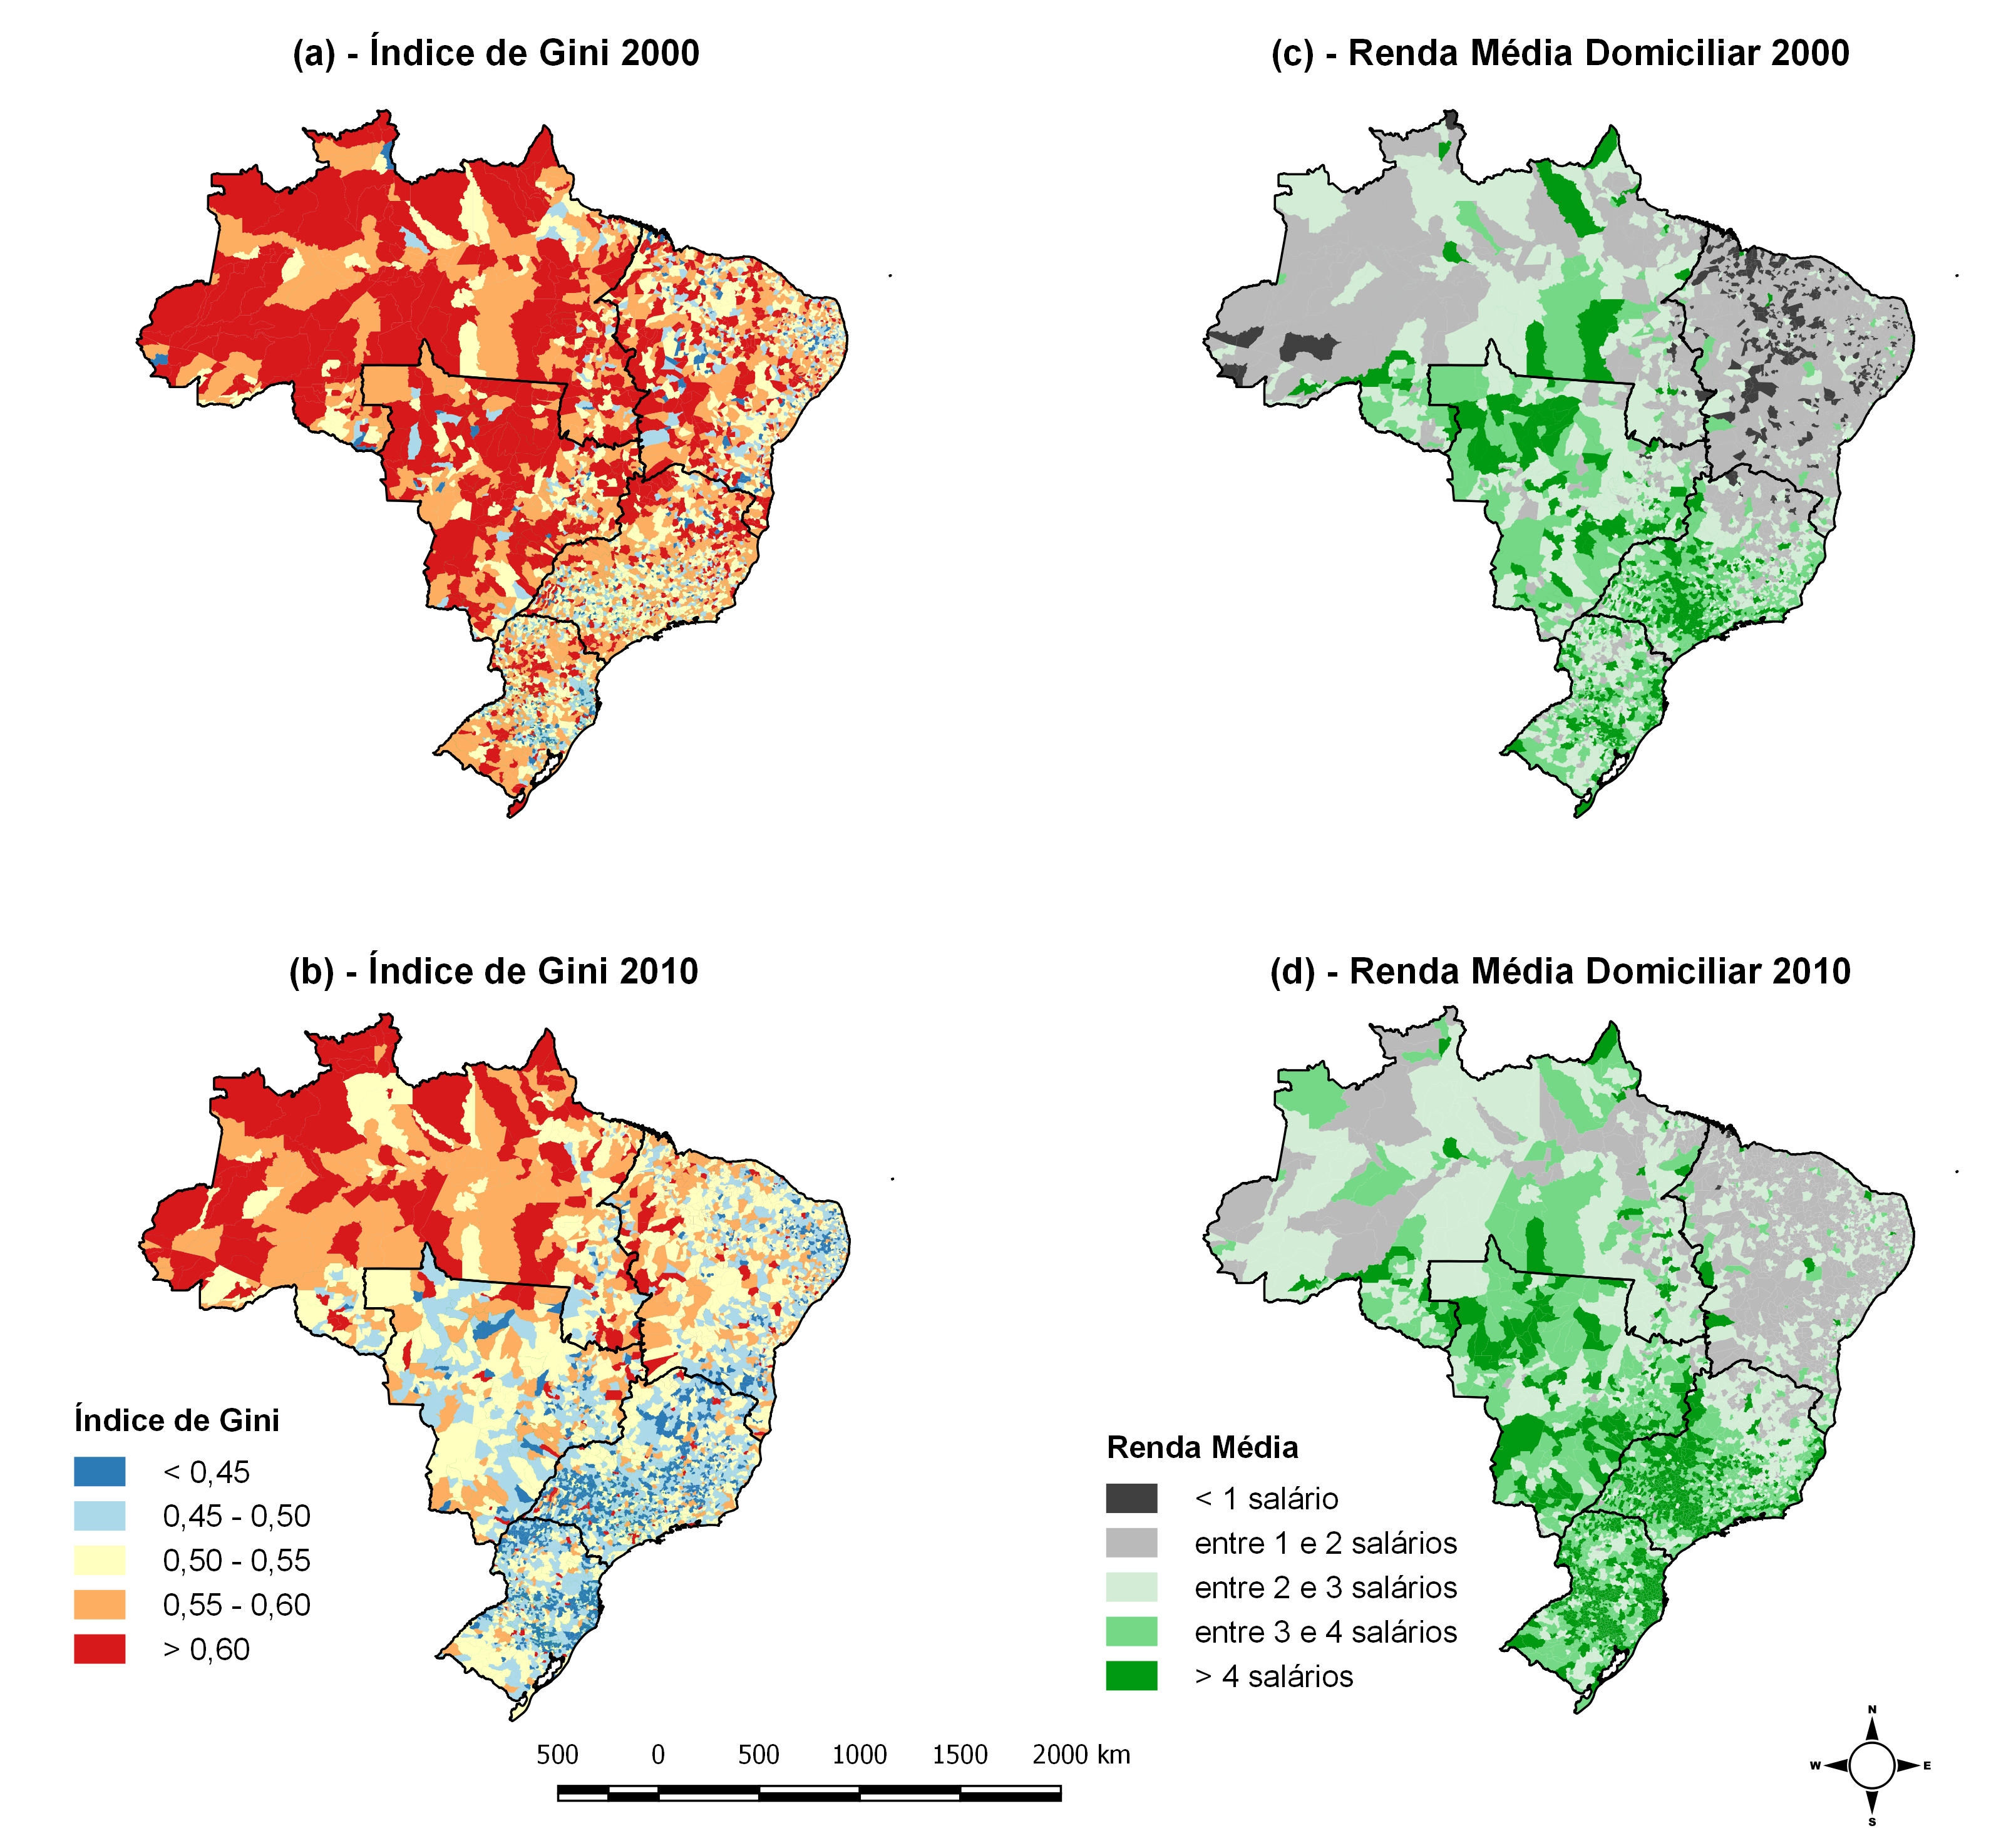
\includegraphics[width=\textwidth]{figs/cap04_mapa_gini_renda.png}
    \caption*{\footnotesize{Fonte: Elaborado pelo autor}}
    \label{fig:cap04:ginicidades}
\end{figure}

Do mesmo modo, as subfiguras \ref{fig:cap04:ginicidades}(c) e \ref{fig:cap04:ginicidades}(d) ilustram os rendimentos médios domiciliares (valores deflacionados para outubro de 2010 pelo INCP) dos municípios brasileiros nos anos de 2000 e 2010. Acerca desses mapas, é evidente o contraste existente no país, no qual cidades das regiões sul, sudeste e centro-oeste apresentam índices de renda média superiores aos demais municípios do norte e nordeste. 

Quantificando esses resultados, aproximadamente 82\% das cidades tiveram redução no coeficiente, sendo que 25\% dessas tiveram uma diminuição acima de 0,1 para o indicador. Observando as subfiguras \ref{fig:cap04:ginicidades}(a) e \ref{fig:cap04:ginicidades}(b) ressalta-se que esses dados de redução não apresentaram tanto impacto nos municípios da região norte em relação as demais regiões. Além disso, os índices de rendimento médio domiciliar para esta região se mantiveram baixo em ambos os anos analisados, evidenciando dessa forma a necessidade de atenção especial para essas cidades no âmbito de políticas públicas.

Analisando a região nordeste, é notória a redução do indicador acerca dos seus municípios. Todavia, realizando uma avaliação comparativa entre índice de Gini e rendimento médio domiciliar, observa-se que embora a região apresente uma melhora na métrica, seus valores de renda média apresentam-se baixos, ou seja, embora a distribuição de renda apresente aparência igualitária a mesma é nivelada por valores baixos em relação a cidades das regiões Sul, Sudeste e Centro-Oeste. 

\pagebreak

Posteriormente, foi analisado o impacto da parcela de aposentadorias e pensões acerca dos resultados encontrados para o índice de Gini nas cidades e estados brasileiros. Primeiramente, optou-se por examinar a sua participação percentual acerca do rendimento mensal per capita de cada unidade federativa do Brasil, podendo ser observado na Figura~\ref{fig:cap04:aposen_pensao_estados}.

Examinando os resultados encontrados, percebe-se que essa parcela tem importante participação no rendimento mensal per capita, com médias estaduais de 15,36\% e 17,63\% para 2000 e 2010 respectivamente. Nota-se também que apenas as unidades federativas do Amapá e do Distrito Federal não tiveram uma variação percentual positiva no ano de 2010 em relação aos dados de 2000, evidenciando uma crescente presença desses benefícios acerca da economia nacional.

\begin{figure}[!ht]
    \centering
    \caption{Participação percentual das rendas de aposentadorias e pensões no total dos rendimentos per capita das unidades federativas brasileiras, 2000 e 2010}
    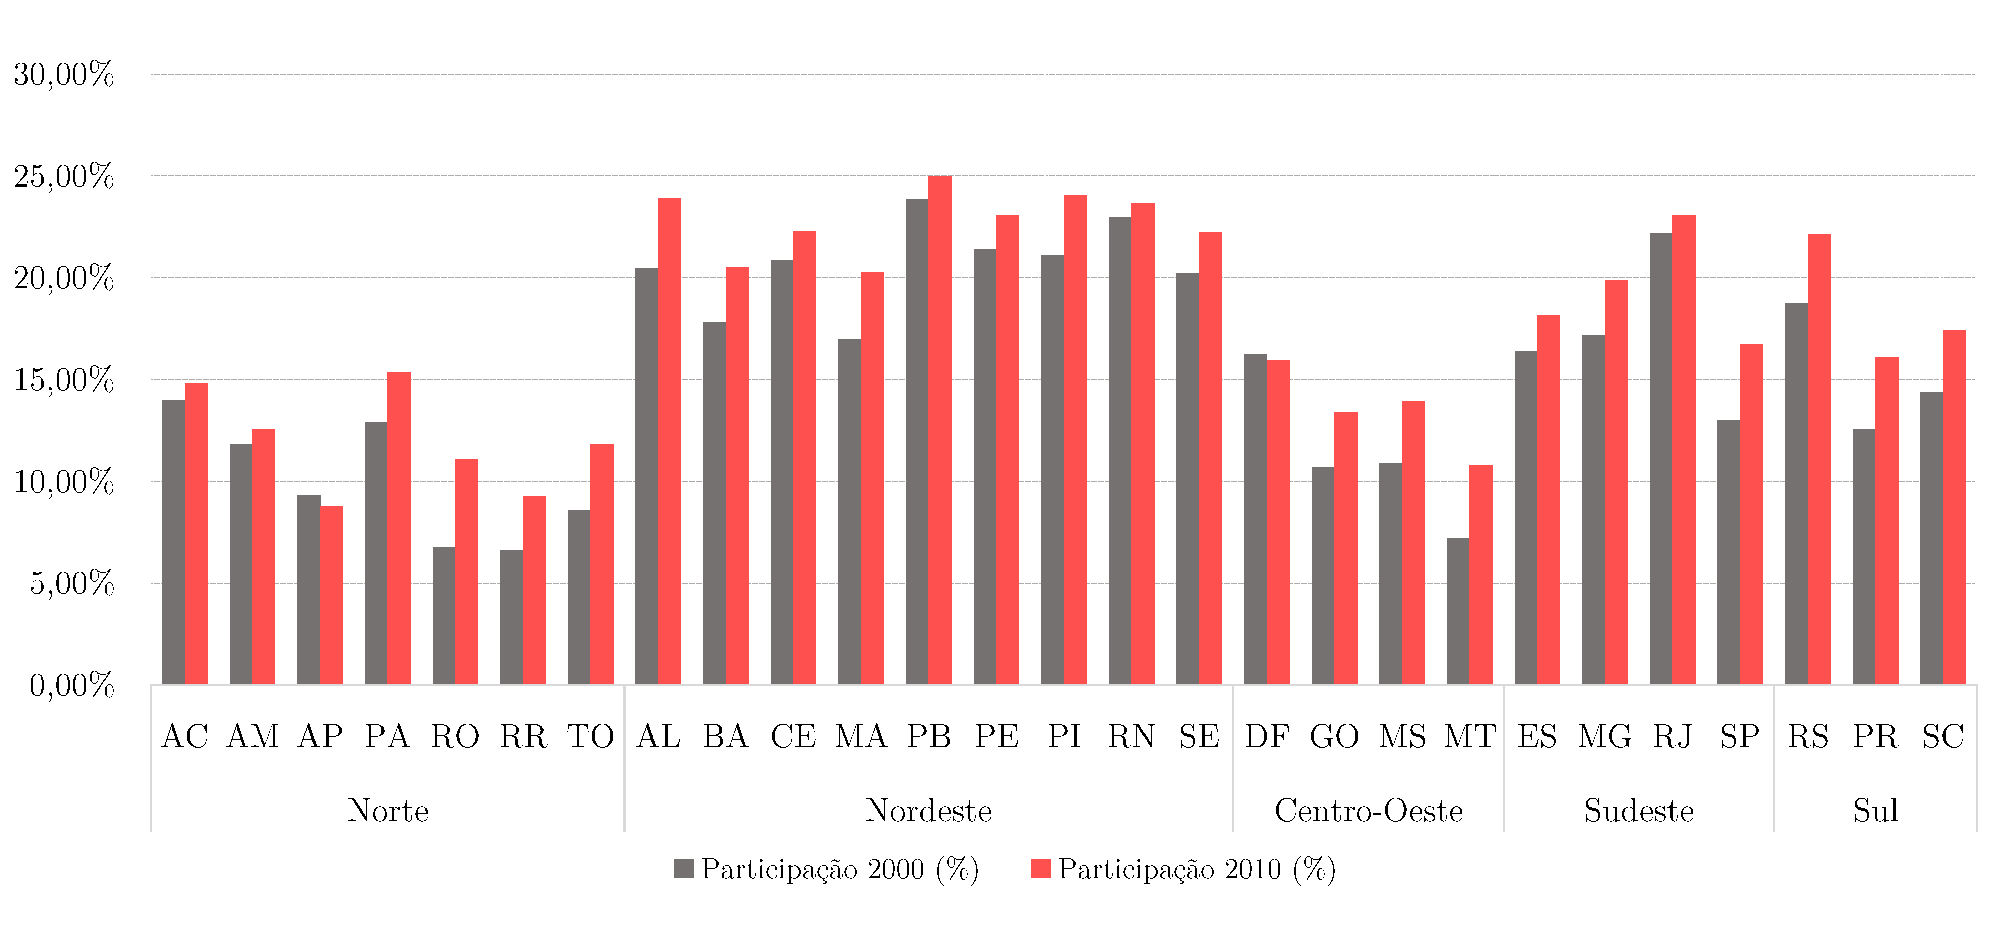
\includegraphics[width=\textwidth]{figs/cap04_aposen_pensao_estados.pdf}
    \caption*{\footnotesize{Fonte: Elaborado pelo autor}}
    \label{fig:cap04:aposen_pensao_estados}
\end{figure}

Em relação a evolução da participação total da parcela entre 2000 e 2010, destacam-se os estados de RO (Rondônia), RR (Roraima) e MT, com uma variação percentual positiva acima de 40\%. Além disso, os estados da região nordeste ganham atenção especial nessa análise, uma vez que em todos as aposentadorias e pensões representam pelo menos 1/5 de todo o rendimento per capita da população. Em escala municipal, a participação desses benefícios no rendimento da população é ainda mais impactante, com aproximadamente 45\% das cidades (2.465 municípios) apresentando pelo menos 1/3 dos rendimentos per capita provenientes dos benefícios citados no ano de 2010.  

Conforme descrito na Equação~\ref{eq:2.13} da Metodologia, a progressividade ($\pi_h$), ou razão concentração, é uma métrica utilizada para aferir a contribuição de uma parcela de rendimento no aumento ou diminuição da desigualdade de renda de uma população. Estudos realizados na literatura identificam que a parcela de aposentadorias e pensões contribui para a concentração de renda no Brasil \cite{cap02_ref22}.

Entretanto, analisando a Tabela~\ref{tab:cap04:progressividadeestados} observa-se que a categoria até um salário mínimo apresenta caráter progressivo ($\pi_h > 0$), colaborando para a diminuição da concentração de renda, para todos os estados brasileiros em ambos os anos examinados. Em contrapartida, as aposentadorias e pensões acima de um salário mínimo se mostram regressivas ($\pi_h < 0$) em todos os estados, indicando uma participação dessa parcela para o aumento da concentração de renda no Brasil.

\begin{table}[!ht]
    \caption{Progressividade ($\pi_h$) da parcela de rendimentos de aposentadorias e pensões por categorias para os estados brasileiros, 2000 e 2010}
    \renewcommand{\arraystretch}{1.4}
    \resizebox{\textwidth}{!}{
    \begin{tabular}{lccccccccc}
    \Xhline{2pt}
     & AC & AL & AM & AP & BA & CE & DF & ES & GO \\ \cline{2-10} 
    até um salário - 2000 & {\color[HTML]{3531FF} 0,8904} & {\color[HTML]{3531FF} 0,7139} & {\color[HTML]{3531FF} 0,9482} & {\color[HTML]{3531FF} 0,9839} & {\color[HTML]{3531FF} 0,7086} & {\color[HTML]{3531FF} 0,7085} & {\color[HTML]{3531FF} 1,2129} & {\color[HTML]{3531FF} 0,9615} & {\color[HTML]{3531FF} 0,9554} \\
    até um salário - 2010 & {\color[HTML]{3531FF} 0,7168} & {\color[HTML]{3531FF} 0,5275} & {\color[HTML]{3531FF} 0,7288} & {\color[HTML]{3531FF} 0,6726} & {\color[HTML]{3531FF} 0,5609} & {\color[HTML]{3531FF} 0,4856} & {\color[HTML]{3531FF} 1,1914} & {\color[HTML]{3531FF} 0,8210} & {\color[HTML]{3531FF} 0,7927} \\
    acima de um salário - 2000 & {\color[HTML]{FE0000} -0,1043} & {\color[HTML]{FE0000} -0,2503} & {\color[HTML]{FE0000} -0,1719} & {\color[HTML]{FE0000} -0,1718} & {\color[HTML]{FE0000} -0,2289} & {\color[HTML]{FE0000} -0,2524} & {\color[HTML]{FE0000} -0,1387} & {\color[HTML]{FE0000} -0,1734} & {\color[HTML]{FE0000} -0,1819} \\
    acima de um salário - 2010 & {\color[HTML]{FE0000} -0,2019} & {\color[HTML]{FE0000} -0,2878} & {\color[HTML]{FE0000} -0,2334} & {\color[HTML]{FE0000} -0,1781} & {\color[HTML]{FE0000} -0,2588} & {\color[HTML]{FE0000} -0,2866} & {\color[HTML]{FE0000} -0,1349} & {\color[HTML]{FE0000} -0,2130} & {\color[HTML]{FE0000} -0,2293} \\ \Xhline{2pt}
     & MA & MG & MS & MT & PA & PB & PE & PI & PR \\ \cline{2-10} 
    até um salário - 2000 & {\color[HTML]{3531FF} 0,5486} & {\color[HTML]{3531FF} 0,9630} & {\color[HTML]{3531FF} 0,9998} & {\color[HTML]{3531FF} 1,0264} & {\color[HTML]{3531FF} 0,8381} & {\color[HTML]{3531FF} 0,6896} & {\color[HTML]{3531FF} 0,8255} & {\color[HTML]{3531FF} 0,5637} & {\color[HTML]{3531FF} 1,0244} \\
    até um salário - 2010 & {\color[HTML]{3531FF} 0,4037} & {\color[HTML]{3531FF} 0,8138} & {\color[HTML]{3531FF} 0,8721} & {\color[HTML]{3531FF} 0,8693} & {\color[HTML]{3531FF} 0,5670} & {\color[HTML]{3531FF} 0,5435} & {\color[HTML]{3531FF} 0,6020} & {\color[HTML]{3531FF} 0,4403} & {\color[HTML]{3531FF} 0,9043} \\
    acima de um salário - 2000 & {\color[HTML]{FE0000} -0,2847} & {\color[HTML]{FE0000} -0,1635} & {\color[HTML]{FE0000} -0,1530} & {\color[HTML]{FE0000} -0,1602} & {\color[HTML]{FE0000} -0,2124} & {\color[HTML]{FE0000} -0,2715} & {\color[HTML]{FE0000} -0,2097} & {\color[HTML]{FE0000} -0,2628} & {\color[HTML]{FE0000} -0,1048} \\
    acima de um salário - 2010 & {\color[HTML]{FE0000} -0,2713} & {\color[HTML]{FE0000} -0,2329} & {\color[HTML]{FE0000} -0,2118} & {\color[HTML]{FE0000} -0,2173} & {\color[HTML]{FE0000} -0,2612} & {\color[HTML]{FE0000} -0,2727} & {\color[HTML]{FE0000} -0,2638} & {\color[HTML]{FE0000} -0,2619} & {\color[HTML]{FE0000} -0,1700} \\ \Xhline{2pt}
     & RJ & RN & RO & RR & RS & SC & SE & SP & TO \\ \cline{2-10} 
    até um salário - 2000 & {\color[HTML]{3531FF} 1,1402} & {\color[HTML]{3531FF} 0,8181} & {\color[HTML]{3531FF} 0,9099} & {\color[HTML]{3531FF} 0,9947} & {\color[HTML]{3531FF} 1,0494} & {\color[HTML]{3531FF} 1,0829} & {\color[HTML]{3531FF} 0,7038} & {\color[HTML]{3531FF} 1,1800} & {\color[HTML]{3531FF} 0,7877} \\
    até um salário - 2010 & {\color[HTML]{3531FF} 1,0064} & {\color[HTML]{3531FF} 0,5769} & {\color[HTML]{3531FF} 0,6994} & {\color[HTML]{3531FF} 0,7557} & {\color[HTML]{3531FF} 0,8935} & {\color[HTML]{3531FF} 0,9628} & {\color[HTML]{3531FF} 0,5785} & {\color[HTML]{3531FF} 1,0513} & {\color[HTML]{3531FF} 0,7044} \\
    acima de um salário - 2000 & {\color[HTML]{FE0000} -0,1008} & {\color[HTML]{FE0000} -0,2492} & {\color[HTML]{FE0000} -0,1095} & {\color[HTML]{FE0000} -0,1463} & {\color[HTML]{FE0000} -0,0955} & {\color[HTML]{FE0000} -0,0726} & {\color[HTML]{FE0000} -0,2429} & {\color[HTML]{FE0000} -0,0026} & {\color[HTML]{FE0000} -0,1976} \\
    acima de um salário - 2010 & {\color[HTML]{FE0000} -0,1711} & {\color[HTML]{FE0000} -0,2726} & {\color[HTML]{FE0000} -0,1775} & {\color[HTML]{FE0000} -0,1652} & {\color[HTML]{FE0000} -0,1675} & {\color[HTML]{FE0000} -0,1603} & {\color[HTML]{FE0000} -0,2710} & {\color[HTML]{FE0000} -0,1273} & {\color[HTML]{FE0000} -0,1873} \\ \Xhline{2pt}
    \end{tabular}}
    \label{tab:cap04:progressividadeestados}
    \caption*{\footnotesize{Fonte: Elaborado pelo autor.}}
\end{table}

\pagebreak

Na Figura~\ref{fig:cap04:progcidades} é exibida a situação da progressividade acerca dos municípios brasileiros. As subfiguras \ref{fig:cap04:progcidades}(a) e \ref{fig:cap04:progcidades}(c), correspondentes à parcela até um salário mínimo para 2000 e 2010, respectivamente, demonstram que o padrão exibido na análise das unidades federativas brasileiras se repete em quase todo território nacional, onde grande parte dos municípios apresentam caráter progressivo ($\pi_h > 0$) para a categoria. Destacam-se as cidades das regiões Norte, Sul, Sudeste, Centro-Oeste para 2000 e Sul, Sudeste e Centro-Oeste para 2010, as quais apresentam maiores índices de progressividade.

\begin{figure}[!ht]
    \centering
    \caption{Progressividade ($\pi_h$) da parcela de rendimentos de aposentadorias e pensões por categorias para os municípios brasileiros, 2000 e 2010}
    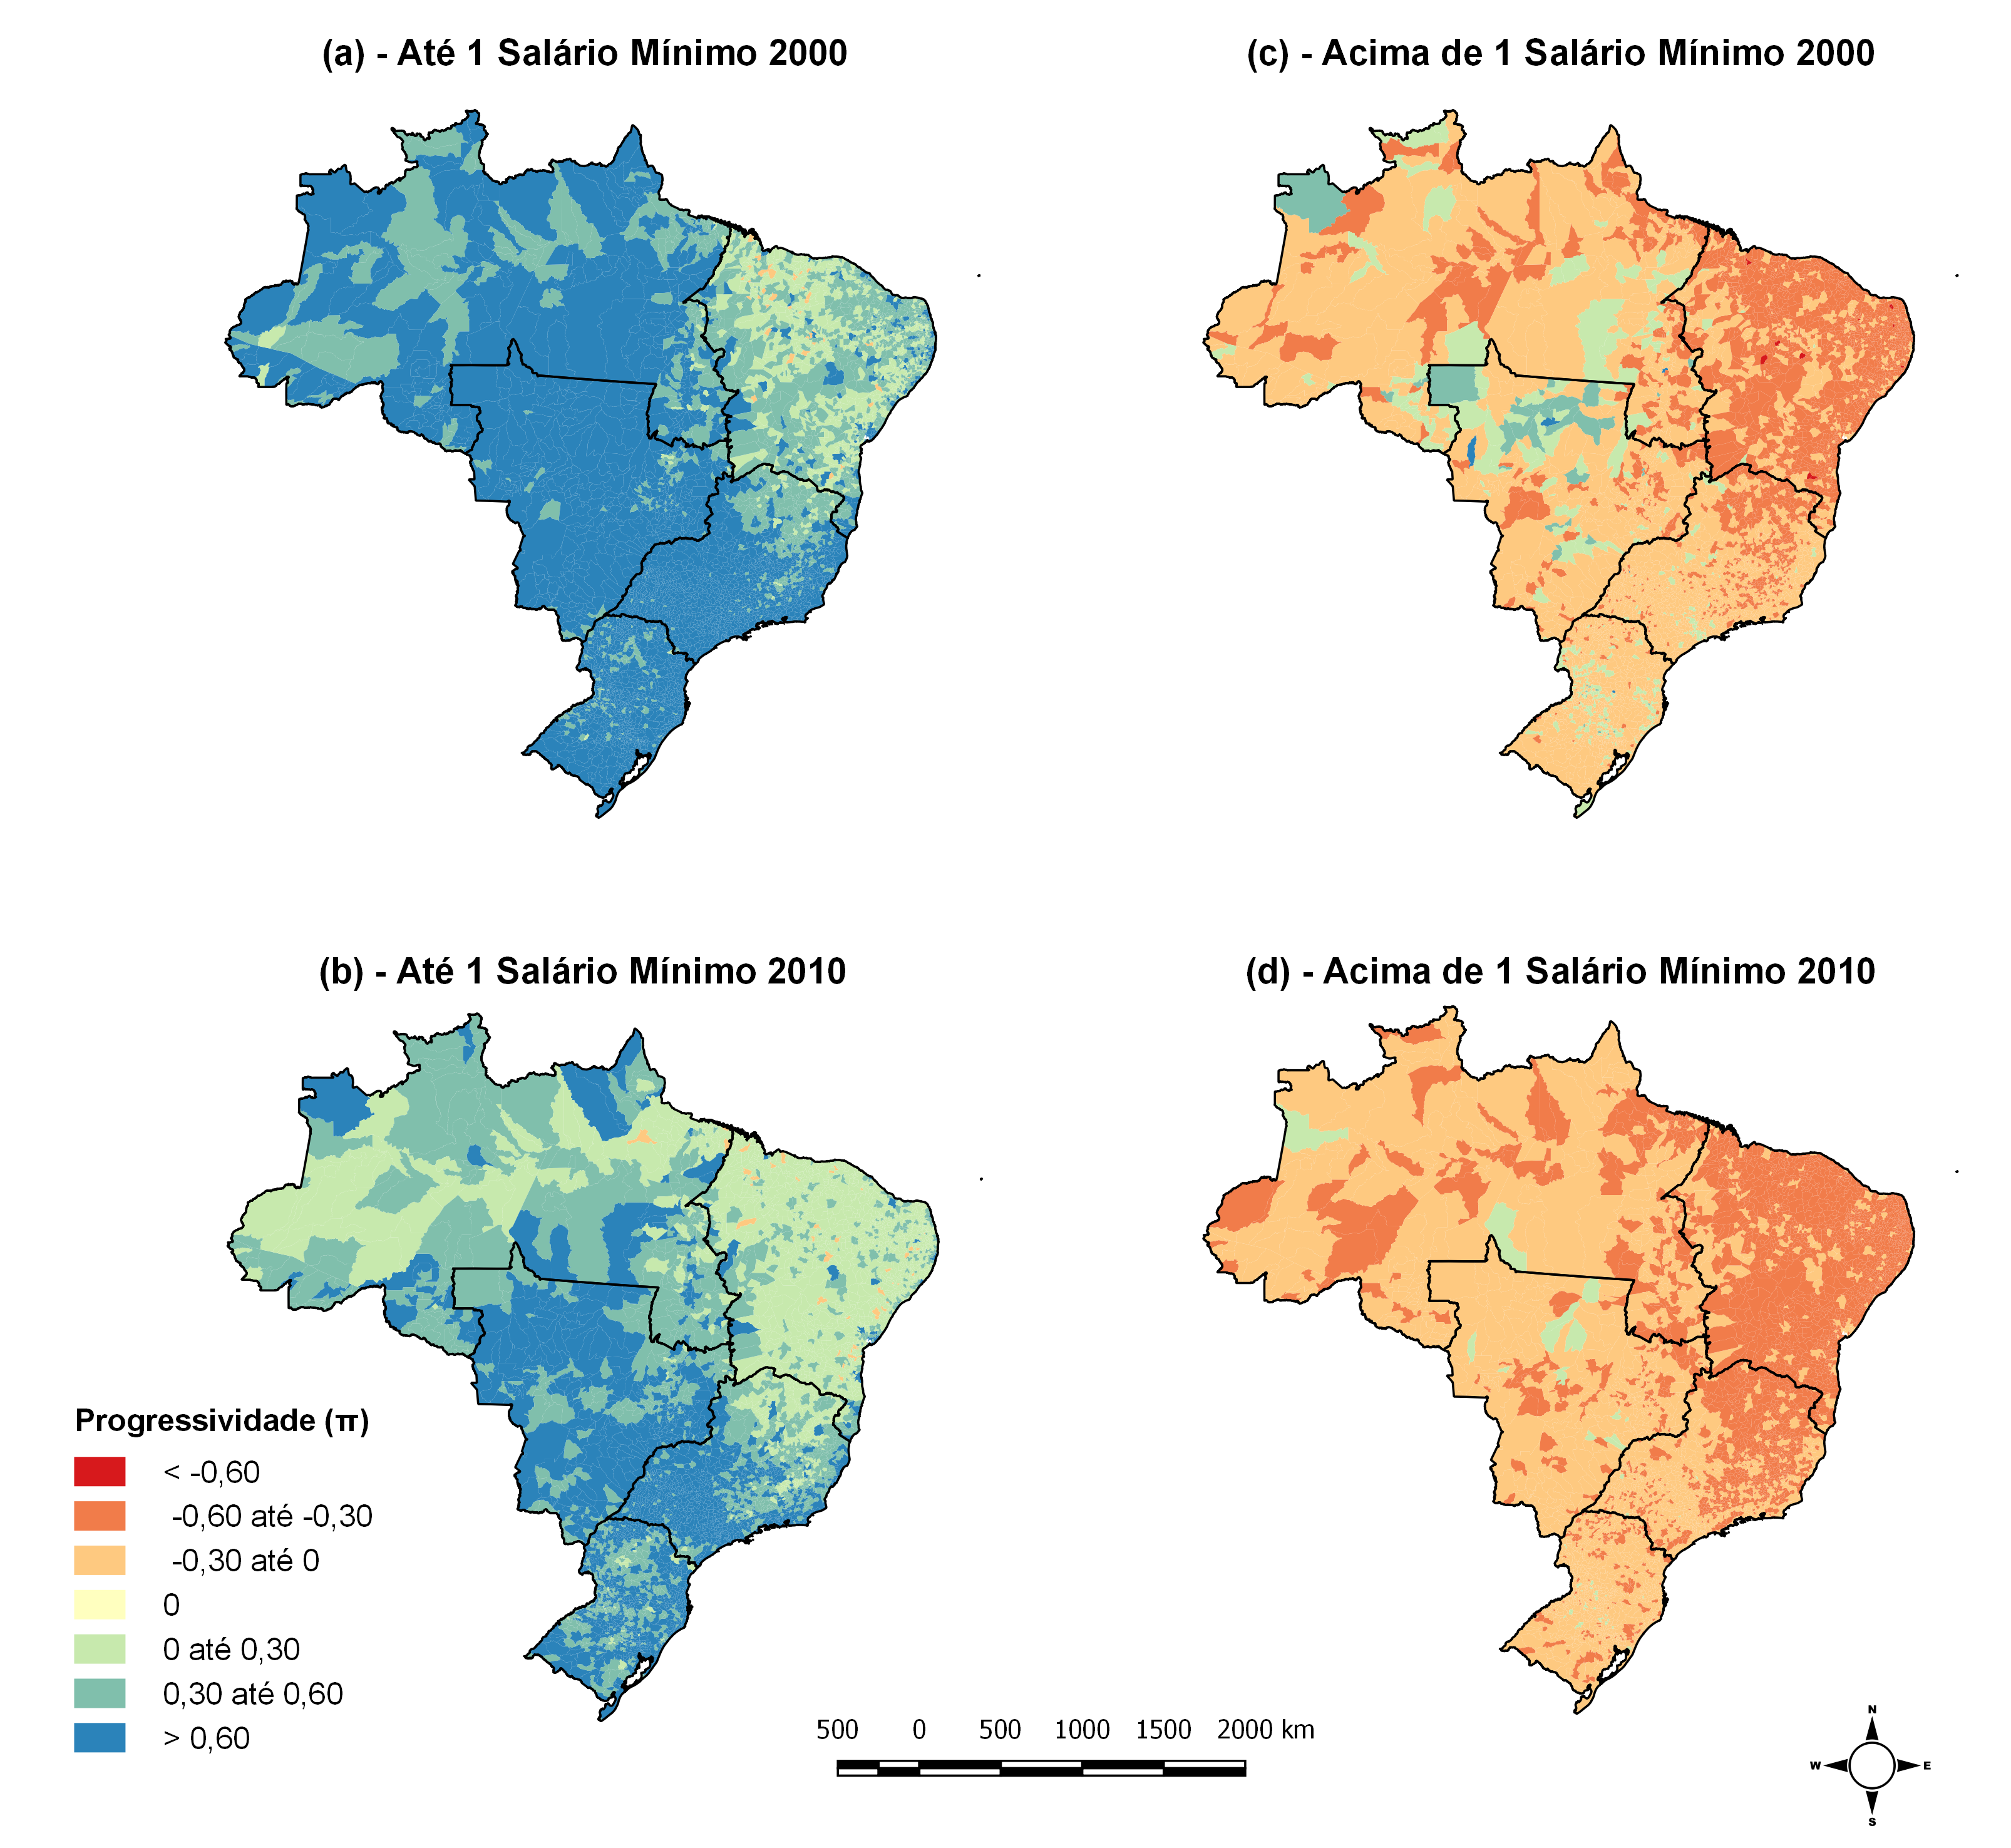
\includegraphics[width=\textwidth]{figs/cap04_mapa_prog_cidades.png}
    \caption*{\footnotesize{Fonte: Elaborado pelo autor}}
    \label{fig:cap04:progcidades}
\end{figure}

Do mesmo modo, as subfiguras \ref{fig:cap04:progcidades}(b) e \ref{fig:cap04:progcidades}(d) ilustram as situações das progressividades para as parcelas de aposentadorias e pensões acima de um salário mínimo nos anos de 2000 e 2010 respectivamente. O caráter regressivo ($\pi_h < 0$) observado em todos as unidades federativas para essa variável se repete acerca de grande parte dos municípios brasileiros, demostrando a importante participação dessa categoria no aumento da desigualdade de rendimentos no país.

As cidades da região nordeste destacam-se em relação as demais regiões, apresentando valores ligeiramente negativos para o indicador na categoria acima de um salário mínimo, e índices baixos na parcela de até um salário em ambos os anos analisados. Tal resultado indica que embora grande parte dos rendimentos nesta região sejam proveniente dessa categoria de benefício, conforme indicado na Figura~\ref{fig:cap04:progcidades}, possivelmente as aposentadorias e pensões acima de um salário estão concentradas na menor parcela de beneficiários, colaborando diretamente para concentração de renda existente nesses municípios. 

Posteriormente, foi avaliada a interdependência estatística existente entre o índice de Gini, os percentuais de participação dos benefícios acerca da composição de renda per capita e as progressividades resultantes para aposentadorias e pensões. Dessa forma, utilizando o coeficiente de Pearson, foram desenvolvidas as matrizes de correlação dos atributos analisados para os anos de 2000 e 2010 exibidas nas Figuras~\ref{fig:cap04:matrixcorr}(a) e \ref{fig:cap04:matrixcorr}(b) respectivamente.

\begin{figure}[!h]
    \centering
    \caption{Matrizes de correlação das variáveis. (a) 2000 (b) 2010}
    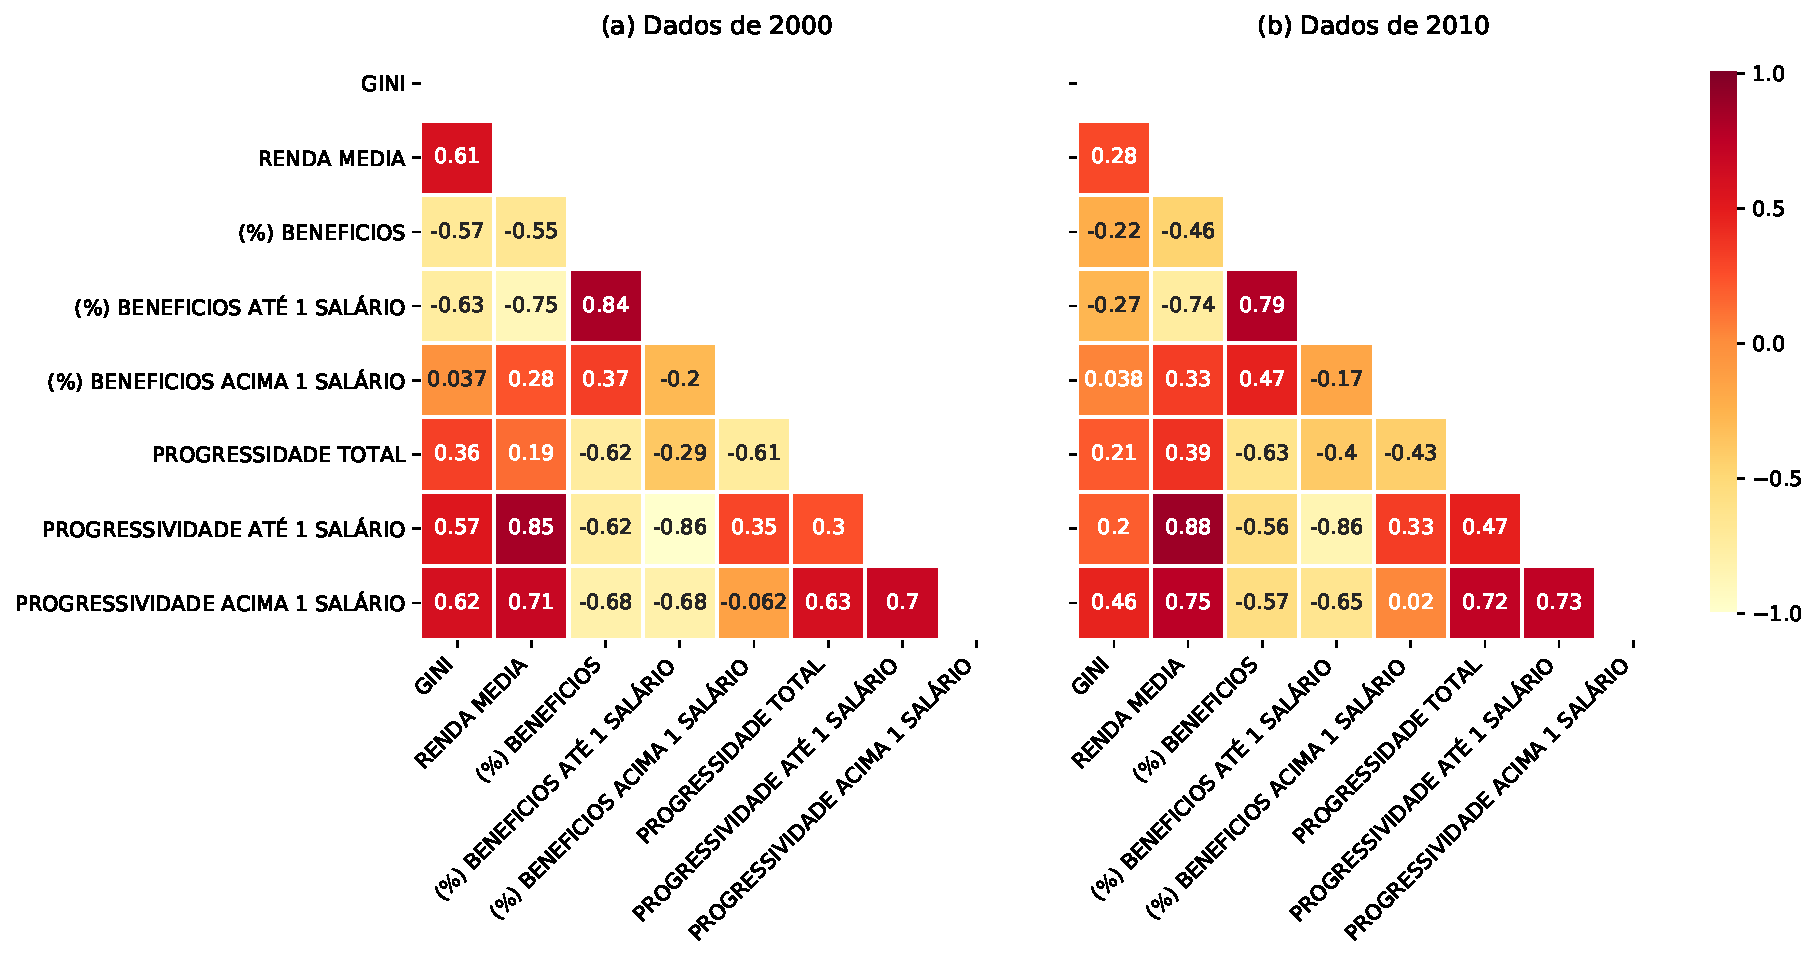
\includegraphics[width=\textwidth]{figs/cap04_corr_matrix.pdf}
    \caption*{\footnotesize{Fonte: Elaborado pelo autor}}
    \label{fig:cap04:matrixcorr}
\end{figure}

Avaliando a imagem, é possível observar uma diminuição na inter-relação existente entre a desigualdade de renda e as demais variáveis examinadas para o intervalo de tempo analisado. Destaca-se a correlação negativa existente entre o índice de Gini e o percentual de participação das aposentadorias e pensões - total e até um salário mínimo - na composição de renda da população. Tal fator indica uma tendencia inversamente proporcional entre as variáveis, ou seja, quanto maior taxa de participação dessa categoria acerca dos municípios brasileiros, menor será a desigualdade de distribuição de riquezas. 

No entanto, evidencia-se a interdependência negativa entre o percentual de participação dos benefícios e a renda média da população, pressupondo que embora essa categoria colabore para equalização de rendimentos, a mesma nivela os valores de renda por baixo. Por outro lado, a correlação existente entre as progressividades e a participação das aposentadorias e pensões demonstram, novamente, o importante papel que esses benefícios possuem na desigualdade de renda existente nos municípios. Todavia, destaca-se a importância de examinar variáveis geográficas, como a distancia das cidades em relação às metrópoles ou suas clientelas, afim de compreender melhor as interdependências existentes.

% --------------------------------------------------------------------------- %

\section{Considerações Finais}\label{cap04:conclusoes}

No presente estudo foi analisada a participação dos benefícios de aposentadorias e pensões na distribuição de renda per capita do Brasil (estados e municípios) nos anos de 2000 e 2010. A partir dos resultados demonstrados para o índice de Gini, conclui-se que embora haja uma heterogeneidade na sua distribuição acerca do território nacional, houve uma melhora no parâmetro, tanto a nível estadual quanto municipal, entre os anos analisados. Paralelamente, perante o cenário relatado anteriormente, o qual expõe a extensão da longevidade da população brasileira e o impacto econômico gerado pelo aumento na distribuição das aposentadorias e pensões, foi comprovado um acréscimo na participação percentual dessa parcela no total de rendimento per capita em todos os estados brasileiros.

No entanto, quando analisadas as participações das aposentadorias e pensões, dividindo-as em categorias (até um salário e acima de um salário), os resultados demonstraram que ambas têm papel divergente em sua contribuição para a concentração de renda. Com um padrão se repetindo em todos os estados – e maioria das cidades brasileiras –, os benefícios acima de um salário apresentaram caráter regressivo ($ \pi_h < 0$), colaborando para um aumento do índice de Gini, destacando-se a maior parte dos municípios do nordeste. Por outro lado, a categoria de benefícios até um salário demonstrou caráter progressivo ($\pi_h > 0$) em todo o país, colaborando para uma desconcentração de renda e decréscimo do índice de Gini.  

Com isso, identifica-se que embora as aposentadorias e pensões colaborem para a concentração de renda no Brasil, conforme apresentado por \cite{cap04_ref7, cap04_ref8, cap04_ref9} , tal fator apresenta caráter contraditório ao segmentarmos os benefícios em diferentes faixas salariais, uma vez que cada categoria colabora de forma diferente acerca da distribuição de renda. Dessa forma, correlacionando tal fator à heterogeneidade que o índice de Gini apresenta no cenário brasileiro, é possível vislumbrar discussões e análises cada vez mais complexas que objetivem equalizar as variáveis relacionadas a essa problemática.

Contudo, destaca-se que relatórios e estudos recentes apontam uma variação positiva para o coeficiente de Gini nos últimos anos, fator diretamente relacionado a crise econômica nacional a qual registrou uma queda de aproximadamente 9\% no PIB entre 2014 e 2016 \cite{cap04_ref19}. Dessa forma, evidencia-se a necessidade de pesquisas com dados atualizados acerca dos municípios brasileiros a fim de mensurar a real situação de distribuição de renda do país, além do impacto que as aposentadorias e pensões causam nessa. Entretanto, os valores de rendimento domiciliar (e dos benefícios que os compõe), a nível municipal, são informações disponibilizadas apenas pelo censo demográfico, impossibilitando a realização de tais análises no presente momento.

Diante disso, como trabalhos futuros, propõem-se a replicação do atual estudo utilizando os dados futuramente disponibilizados pelo IBGE relacionados ao censo demográfico de 2020, a exploração de outros indicadores econômico-sociais (como por exemplo o índice de \textit{Theil}), a aplicação técnicas de inteligência computacional para a extração de novos \textit{insights} acerca da problemática e a utilização de métodos estatísticos espaciais (como o Índice de Moran \cite{cap04_ref20}) a fim de compreender melhor a autocorrelação existente na dispersão das variáveis entre os municípios.


\chapter{Os Impactos da Reforma Previdenciária Acerca das Concessões de Benefícios de Aposentadoria}

% --------------------------------------------------------------------------- %
\section{Considerações Iniciais}

Conforme demonstrado no capítulo anterior, as aposentadorias e pensões compreendem uma importante categoria na composição de renda da população brasileira, impactando diretamente na desigualdade socioeconômica nacional. Dessa forma, acerca da magnitude social que esses benefícios proporcionam, evidencia-se que alterações nas regras de acesso ao regime previdenciário, como as previstas pela PEC 287/16\footnote{Disponível em: <https://www.camara.leg.br/proposicoesWeb/fichadetramitacao?idProposicao=2119881> Acesso em: 14 Jan, 2020}) ou PEC 6/2019\footnote{Disponível em: <https://www.camara.leg.br/proposicoesWeb/fichadetramitacao?idProposicao=2192459> Acesso em: 14 Jan, 2020}, tendem a apresentar importantes consequências acerca da sociedade. 

Embora diversos trabalhos abordem a sustentabilidade da Previdência Social, estimando projeções econômicas a curto e longo prazo \cite{cap03_ref5, cap05_ref9}, ou a confiabilidade dos resultados divulgados pelo governo para justificar as referidas reformas \cite{cap05_ref10, cap01_ref3}, observa-se na literatura a ausência de pesquisas que investiguem os efeitos que tais alterações nas regras de acesso causariam nas concessões de aposentadorias.

Dessa forma, esse estudo de caso objetivou avaliar os impactos que a reforma prevista pela PEC 06/2019 pode causar no cenário previdenciário brasileiro acerca das concessões dos benefícios de aposentadoria. Especificamente, visou, através de uma abordagem de ciência de dados, utilizar os dados oficiais disponibilizados pela CPI da Previdência, pelo IBGE e pelo Anuário Estatístico da Previdência Social, para simular os efeitos que a PEC 06/2019 causariam no período de 1995 a 2016 se a mesma já estivesse em vigor no momento em que cada benefício foi concedido.

Para isso, esse capítulo foi dividido em 4 subseções incluindo esta breve introdução. Em seguida, na subseção~\ref{cap05:metodologia}, será abordada a metodologia para o desenvolvimento das análises realizadas, evidenciando a arquitetura utilizada para armazenamento dos dados, validação das informações disponibilizadas e detalhes da simulação proposta. Na subseção~\ref{cap05:resultados} serão discutidos os principais resultados encontrados, finalizando o estudo na subseção~\ref{cap05:conclusoes} com as considerações finais. 

% --------------------------------------------------------------------------- %
\section{Metodologia Utilizada}\label{cap05:metodologia}

Para o desenvolvimento do estudo proposto foi estabelecida uma sequência de etapas relacionadas a análise de dados, semelhante ao estudo anterior. No entanto, devido à natureza da problemática, e ao fato da pesquisa necessitar de outras fontes de informações para a abstração de melhores \textit{insights}, foi adotada uma estratégia metodológica diferente. Sendo assim, como forma de otimizar a organização, armazenamento e consultas nos dados, foi elaborado uma estrutura de \textit{Data Warehouse}\footnote{Data warehouse compreende uma organização para banco de dados comumente utilizada em inteligência de negócios. Sua principal característica esta relacionada ao armazenamento de grandes quantidade dados, de diferentes fontes, em uma arquitetura que possibilite a realização de consultas complexas com maior grau de facilidade.} contendo todas as bases de dados inerentes ao estudo. A Figura~\ref{fig:cap05:metodologia} exibe o fluxo de desenvolvimento deste estudo de caso, contendo cada uma das etapas realizadas seguido por um grau de detalhamento mais aprofundado acerca dessa seção.

\begin{figure}[!ht]
    \centering
    \caption{Fluxograma de desenvolvimento do segundo estudo de caso}
    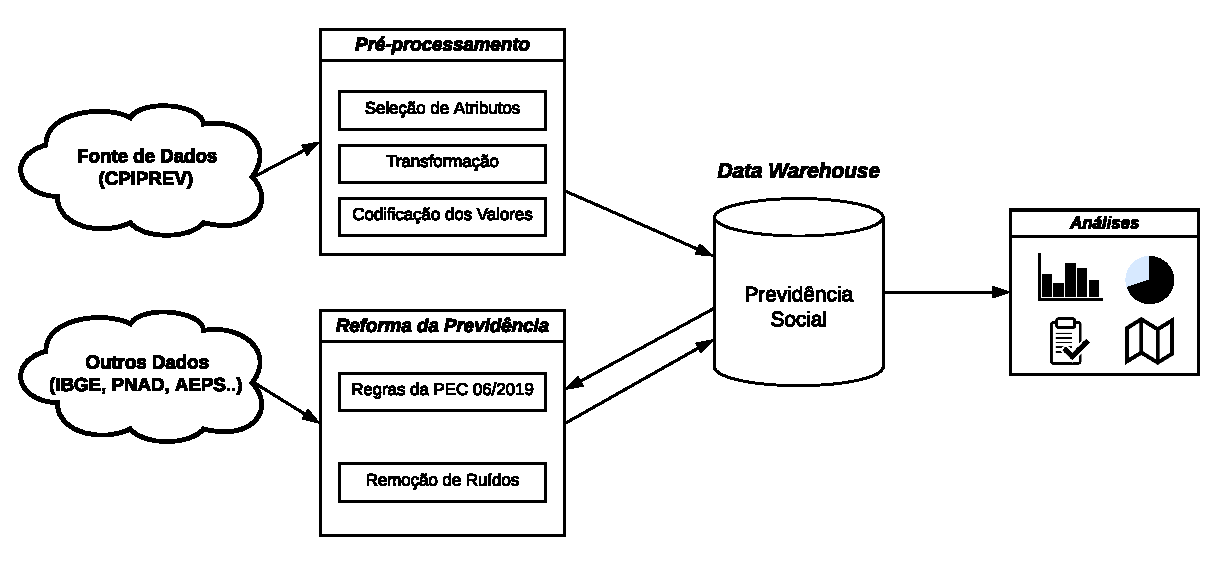
\includegraphics[width=\textwidth]{figs/cap05_metodologia_estudo02.pdf}
    \caption*{\footnotesize{Fonte: Elaborado pelo autor}}
    \label{fig:cap05:metodologia}
\end{figure}

\subsection{Origem dos Dados e Elaboração do \textit{Data Warehouse}}

O estágio inicial do procedimento metodológico deste estudo norteou-se na aquisição dos microdados previdenciários necessários para a reprodução da PEC 06/2019. Sendo assim, após a divulgação do trabalho de \cite{cap05_ref9}, foram solicitadas as informações ausentes nos anexos das LDOs, necessárias para a reprodução dos seus cálculos. Dessa forma, o Ministério da Fazenda disponibilizou os dados referentes a aposentadorias e pensões no site\footnote{Disponível em: <https://legis.senado.leg.br/comissoes/docsRecCPI?codcol=2093> Acesso em: 17 Fev, 2020} CPI da Previdência de 2017, enumerados pelos documentos DOC090 e DOC097.

Esses documentos compreendem séries históricas de dados relacionados a concessão de benefícios de diversas espécies, sendo as principais: aposentadorias por tempo de contribuição (espécie 42), por tempo de contribuição especial (espécies 46 e 57), por idade (espécie 41), por invalidez (espécie 32), além dos benefícios de pensão por morte (espécie 21) e auxílio doença (espécie 31). A Tabela~\ref{tab:cap05:dadosprevidencia} exibe um breve resumo acerca dos dados disponibilizados pela CPI da Previdência de 2017.

\begin{table}[!h]
    \caption{Informações sobre os microdados disponibilizados pela CPI da Previdência de 2017.}
    \resizebox{\textwidth}{!}{
  \begin{tabular}{|cc|c|c|}
    \hline
    \multicolumn{1}{|c|}{\textbf{Origem}} & \textbf{Arquivos} & \textbf{Nº de Registros} & \textbf{Descrição} \\ \hline
    \multicolumn{1}{|c|}{\multirow{2}{*}{DOC090}} & APOSENTADORIAS.csv & 46.545.767 & \begin{tabular}[c]{@{}c@{}}Benefícios de Aposentadorias \\ (42, 46, 57, 41 e 32) e Auxílio 31 \\ concedidos entre 2000 e 2015\end{tabular} \\ \cline{2-4} 
    \multicolumn{1}{|c|}{} & PENSAO.csv & 5.647.457 & \begin{tabular}[c]{@{}c@{}}Benefícios de Pensão da espécie 21\\ concedidas entre 2000 e 2015\end{tabular} \\ \hline
    \multicolumn{1}{|c|}{\multirow{2}{*}{DOC097}} & SEN\_MICRODADOS01.APO.AUX.csv & 57.955.872 & \begin{tabular}[c]{@{}c@{}}Benefícios de Aposentadorias \\ (42, 46, 57, 41, 32 e 92) e Auxílios\\ (91 e 31) concedidos entre 1995 e 2016\end{tabular} \\ \cline{2-4} 
    \multicolumn{1}{|c|}{} & SEN\_MICRODADOS02\_PENS.csv & 7,964,185 & \begin{tabular}[c]{@{}c@{}}Benefícios de Pensão por Morte\\ (21, 93) concedidos entre 1995 e 2016\end{tabular} \\ \hline
     &  & \textbf{118.113.281} &  \\ \hline
  \end{tabular}}
    \label{tab:cap05:dadosprevidencia}
    \caption*{\footnotesize{Fonte: Elaborado pelo autor.}}
\end{table}

Para a realização das análises e simulações propostas, optou-se por utilizar o arquivo SEN\_MICRODADOS01.APO.AUX.csv devido ao fato desse agregar informações relacionadas às principais espécies de aposentadorias em um maior intervalo de tempo. Assim sendo, a base de dados foi inserida na estrutura de \textit{Data Warehouse} dividindo a base de dados em diferentes tabelas do tipo FATO e DIMENSAO, sendo as primeiras responsáveis pelo conteúdo bruto dos dados (registros de aposentadorias) e as segundas por dados complementares (formato de datas, espécies de aposentadorias, tipo de clientela, etc) utilizadas principalmente em consultas mais específicas e complexas.

Para a elaboração da estrutura da \textit{Data Warehouse} e bancos de dados, além da criação das tabelas FATO e DIMESAO e conversão dos dados contidos no arquivo .csv (\textit{comma separated values}) em registros, foi utilizado o \textit{software} de código aberto \textit{Pentaho Data Integration} (PDI)\footnote{Disponível em: <https://community.hitachivantara.com/s/article/data-integration-kettle> Acesso em: 18 Fev, 2020}. Devido ao fato dessa ferramenta ser fortemente utilizada na área de inteligência de negócios, a mesma promove um conjunto de funcionalidades relacionadas a análise de dados tais como suporte à linguagem Structured Query Language (SQL) e comunicação com os principais sistemas gerenciadores de bancos de dados. 

Diante disso, foram utilizadas funcionalidades do PDI e da linguagem de programação SQL para realizar uma etapa de pré-processamento dos dados. Essa etapa compreendeu a seleção dos atributos relevantes para o estudo e transformações acerca dos microdados, como por exemplo codificação de valores textuais em numéricos para diminuir a demanda computacional necessária. Por fim, os microdados resultantes, correspondentes a série histórica de benefícios de aposentadorias/auxílios concedidos entre os anos de 1995 e 2016, foram armazenados em SGBD PostgreSQL. O Apêndice~\ref{apendice:a} apresenta, resumidamente, os principais metadados presentes nesta base de dados, podendo ser encontrado ao final deste documento.
	
Diante disso, a partir da utilização de funcionalidades do PDI e da linguagem de programação SQL, foi realizada uma etapa de pré-processamento dos dados, a qual compreendeu a seleção dos atributos relevantes para o estudo e transformações acerca dos microdados, como a codificação dos valores textuais em numéricos. Posteriormente, os dados resultantes, correspondentes a série histórica de benefícios de aposentadorias/auxílios concedidos entre os anos de 1995 e 2016, foram armazenados em um SGBD PostgreSQL.

Destaque-se que a utilização de uma estrutura de \textit{Data Warehouse} não possibilita a inserção ou remoção de registros no banco de dados de maneira automática e dinâmica. Para tal funcionalidade, o administrador da arquitetura – utilizando técnicas de \textit{Extract, Transfom and Load} (ETL) responsáveis por extrair, transformar/pré-processar e carregar dados de diferentes origens em bancos de dados – promove a atualização do \textit{Data Warehouse} de acordo com a demanda necessária \cite{cap05_ref12, cap05_ref13}. Todavia, devido à natureza da aplicação realizada nesse estudo não promover uma atualização dinâmica nos dados, fator justificado pela dificuldade de acesso a microdados recentes de concessões de aposentadorias, essa ferramenta apresentou-se promissora uma vez que possibilita consultas mais complexas e com menor grau de dificuldade.  

\subsection{Análise Exploratória}

Uma vez que o desenvolvimento do \textit{Data Warehouse} responsável pelo armazenamento dos microdados previdenciários foi realizado, constatou-se a necessidade de efetuar uma análise exploratória acerca dos dados, objetivando, principalmente, compreender o seu conteúdo e avaliar a confiabilidade das informações disponibilizadas. Dessa forma, foram utilizados os microdados fornecidos pelo DATAPREV para recalcular os resultados divulgados pelo Anuário Estatístico da Previdência Social (AEPS)\footnote{O AEPS foi criado em 1992 e é responsável por disponibilizar para a populações dados estatísticos e básicos referentes a situação dos benefícios mantidos pelo INSS e sobre suas arrecadações de contribuições previdenciárias \cite{cap05_ref14}}. Inicialmente foi elaborada uma série histórica comparativa referentes a concessão dos benefícios de aposentadorias. A Figura~\ref{fig:cap05:aepsvsprev}(a) ilustra o comportamento de ambas as fontes de dados para o intervalo de 1995-2016. Por sua vez, a Figura~\ref{fig:cap05:aepsvsprev}(b) exibe o erro percentual existente entre as duas, enfatizando o ano de 1995, o que apresentou uma diferença acima de 8\% entre dados disponibilizados pela CPI e o AEPS daquele ano.

\begin{figure}[!ht]
    \centering
    \caption{(a) Comparação entre os dados disponibilizados pela CPI da Previdência e as informações contidas no APES. (b) Erro percentual.}
    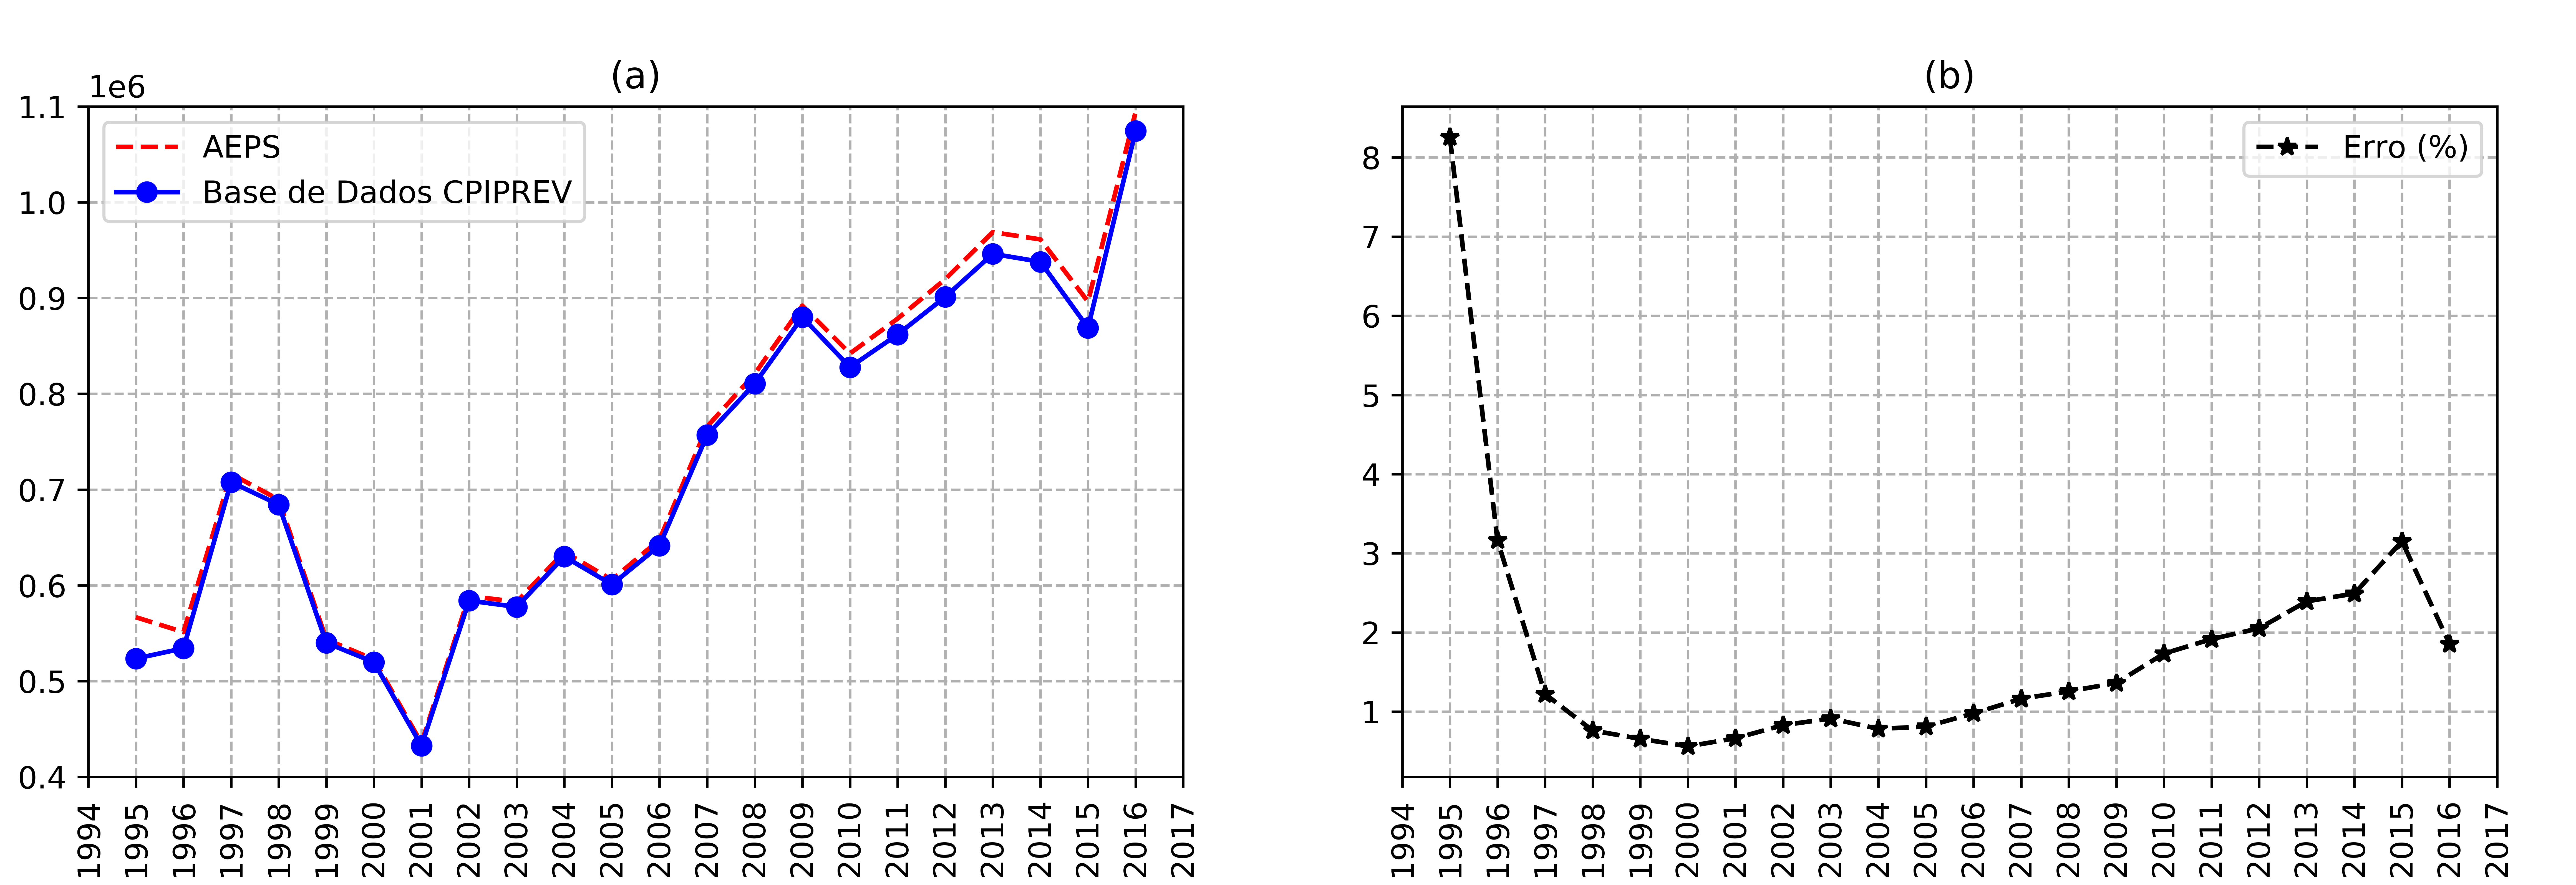
\includegraphics[width=\textwidth]{figs/cap05_apes_vs_cpiprev.png}
    \caption*{\footnotesize{Fonte: Elaborado pelo autor}}
    \label{fig:cap05:aepsvsprev}
\end{figure}

Similarmente, foi reproduzido um dos resultados contidos no AEPS de 2016, intitulado "A.1 - Quantidade de benefícios concedidos, por clientela, segundo os grupos de espécies - 2014/2016", contido na página 21\footnote{Disponível em: <http://sa.previdencia.gov.br/site/2018/08/aeps2016.pdf> Acesso em: 5 de Mar, 2020}, utilizando os microdados disponibilizados pelo DATAPREV. Com isso, conforme exibido na Tabela~\ref{fig:cap05:comparacaoaposen}, notou-se uma pequena variação entre os resultados, proveniente, possivelmente, de ações jurídicas relacionadas a concessões de benefícios, ou seja, contribuintes que deram entrada em benefícios e tiveram retorno após a data de disponibilização dos dados pela CPI da previdência. 

\begin{table}[!h]
    \caption{Comparação entre os dados disponibilizados pelo DATAPREV e as informações contidas no APES: Quantidade de benefícios concedidos por grupos de espécies entre 2014/2016}
    \resizebox{\textwidth}{!}{
    \begin{tabular}{|l|c|c|c|c|c|c|}
        \hline
        \multicolumn{1}{|c|}{\multirow{2}{*}{\textbf{Espécie}}} & \multicolumn{3}{c|}{\textbf{AEPS}} & \multicolumn{3}{c|}{\textbf{DATAPREV}} \\ \cline{2-7} 
        \multicolumn{1}{|c|}{} & \textbf{2014} & \textbf{2015} & \textbf{2016} & \textbf{2014} & \textbf{2015} & \textbf{2016} \\ \hline
        Aposentadorias & 1.150.880 & 1.058.151 & 1.263.974 & 1.115.107 & 1.058.379 & 1.290.267 \\ \hline
        - Tempo de Contribuição & 315.542 & 320.460 & 432.033 & 315.483 & 320.414 & 439.850 \\ \hline
        - Idade & 645.687 & 575.841 & 662.366 & 645.744 & 575.886 & 674.338 \\ \hline
        - Invalidez & 189.651 & 161.850 & 169.575 & 189.880 & 162.079 & 176.079 \\ \hline
    \end{tabular}}
    \caption*{\footnotesize{Fonte: Elaborado pelo autor}}
    \label{fig:cap05:comparacaoaposen}
\end{table}

Posteriormente, após validar a confiabilidade dos dados utilizados, foi estimada a quantidade de registros existentes na base de dados classificando-os por espécies de benefícios. Dessa forma, a Figura~\ref{fig:cap05:percentapo} exibe um gráfico de barras contendo os percentuais de participação de cada categoria na base de dados, enfatizando as aposentadorias das espécies 42, 46, 57, 41, 32 e 92 (34,62\% do total) correspondentes aos benefícios diretamente atingidos pela reforma previdenciária prevista na PEC 06/2019.

\begin{figure}[!h]
    \centering
    \caption{Percentual de participação dos benefícios da base dados classificados por espécie.}
    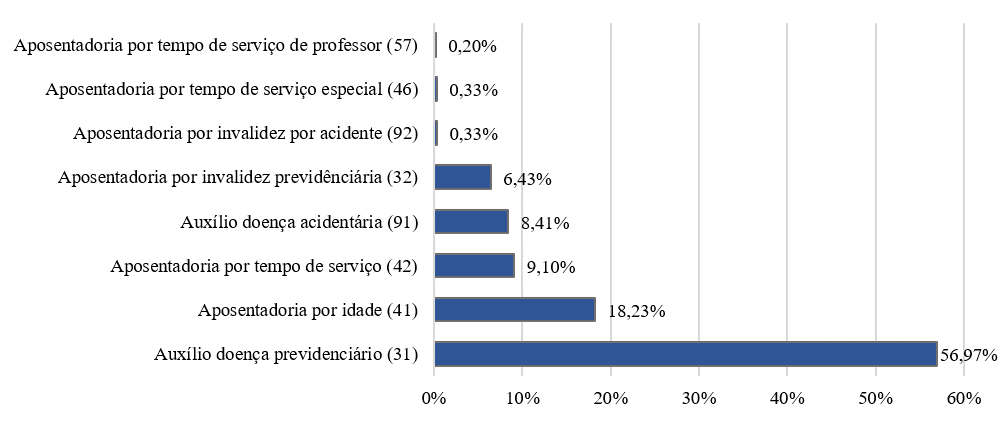
\includegraphics[width=\textwidth]{figs/cap05_percentual_especies.png}
    \caption*{\footnotesize{Fonte: Elaborado pelo autor}}
    \label{fig:cap05:percentapo}
\end{figure}

Em contrapartida, quando analisada a proporção de aposentadorias concedidas classificando-as por sexo, identificou-se relativo grau de equilíbrio com 55,06\% dos segurados correspondendo ao sexo masculino, 44,93\% ao feminino e 0,01\% com o sexo ignorado/indefinido. No entanto, devido a natureza das simulações propostas, a última categoria foi desconsiderada visto que as regras previstas na PEC 06/2019 não incorporavam diretrizes relacionadas a sexo indefinido. 

Após a realização da análise exploratória e validação das informações existentes no banco de dados, contatou-se a possibilidade de simular a reforma da previdenciária conforme previsto nos objetivos deste estudo. Além disso, outras análises estatísticas e quantitativas mais detalhadas foram realizadas a fim de compreender melhor o conteúdo desses microdados. Foram disponibilizadas as informações referentes a essas análises complementares, a documentação necessária para sua replicação os códigos fontes utilizados para cada cálculo e consulta realizados acerca da base de dados no repositório do projeto disponível na plataforma GitHub\footnote{Disponível em: <https://github.com/andrespp/ds-prev> Acesso em: 3 Mai, 2020}.

\subsection{Simulação da Reforma Previdenciária (PEC06/2019)}

Após a realização das etapas anteriores, e utilizando dados públicos disponibilizados pelo IBGE e AEPS, foi elaborada e incorporada uma nova base de dados ao \textit{Data Warehouse} referente a uma simulação das regras previstas pela reforma da previdência prevista na PEC 06/2019\footnote{As regras utilizadas são referentes à proposta em vigor no dia 15/06/2019, podendo eventualmente ter sofrido alterações após a publicação do trabalho.}. A Tabela~\ref{fig:cap05:regraspec} exibe de forma resumida as diretrizes previstas pela reforma para as principais espécies de benefícios em relação a idade mínima e tempo de contribuição em anos. 

\begin{table}[!h]
    \centering
    \caption{Regras para obtenção de aposentadorias propostas pela PEC 06/2019.}
    \newcolumntype{P}[1]{>{\centering\arraybackslash}p{#1}}
    \begin{tabular}{|P{3cm}|P{2.2cm}|P{2.2cm}|P{2.2cm}|P{2.2cm}|}
    \hline
    \multirow{2}{*}{\textbf{Espécie}} & \multicolumn{2}{c|}{\textbf{Idade}} & \multicolumn{2}{c|}{\textbf{Tempo de Contribuição}} \\ \cline{2-5} 
     & \textbf{Mulher} & \textbf{Homem} & \textbf{Mulher} & \textbf{Homem} \\ \hline
    Urbana (41/42) & 62 & 65 & 15 & 20 \\ \hline
    Rural (41/42) & 55 & 60 & \multicolumn{2}{c|}{15} \\ \hline
    Professor (57) & 57 & 60 & \multicolumn{2}{c|}{25} \\ \hline
    Especial (46) & \multicolumn{2}{c|}{55} & \multicolumn{2}{c|}{15} \\ \hline
    Especial (46) & \multicolumn{2}{c|}{58} & \multicolumn{2}{c|}{20} \\ \hline
    Especial (46) & \multicolumn{2}{c|}{60} & \multicolumn{2}{c|}{25} \\ \hline
    \end{tabular}
    \caption*{\footnotesize{Fonte: Elaborado pelo autor}}
    \label{fig:cap05:regraspec}
\end{table}

Essa nova base de dados, além de compreender o universo de registros existentes no banco de dados da previdência, agrega novos atributos referentes a projeções de como tais benefícios se comportariam caso a reforma já estivesse em vigor no momento em que cada aposentadoria foi concedida\footnote{A simulação não considera regras de transição, mas sim as regras finais para concessão de cada benefício.}. Na Figura~\ref{fig:cap05:fluxograma} é possível visualizar, de forma resumida, a lógica utilizada para a realização da simulação proposta através de um fluxograma, o qual terá um maior grau de detalhamento das tarefas realizadas no decorrer desta subseção. 

\newpage

\begin{figure}[!h]
    \centering
    \caption{Fluxograma da simulação da reforma previdenciária PEC 06/2016}
    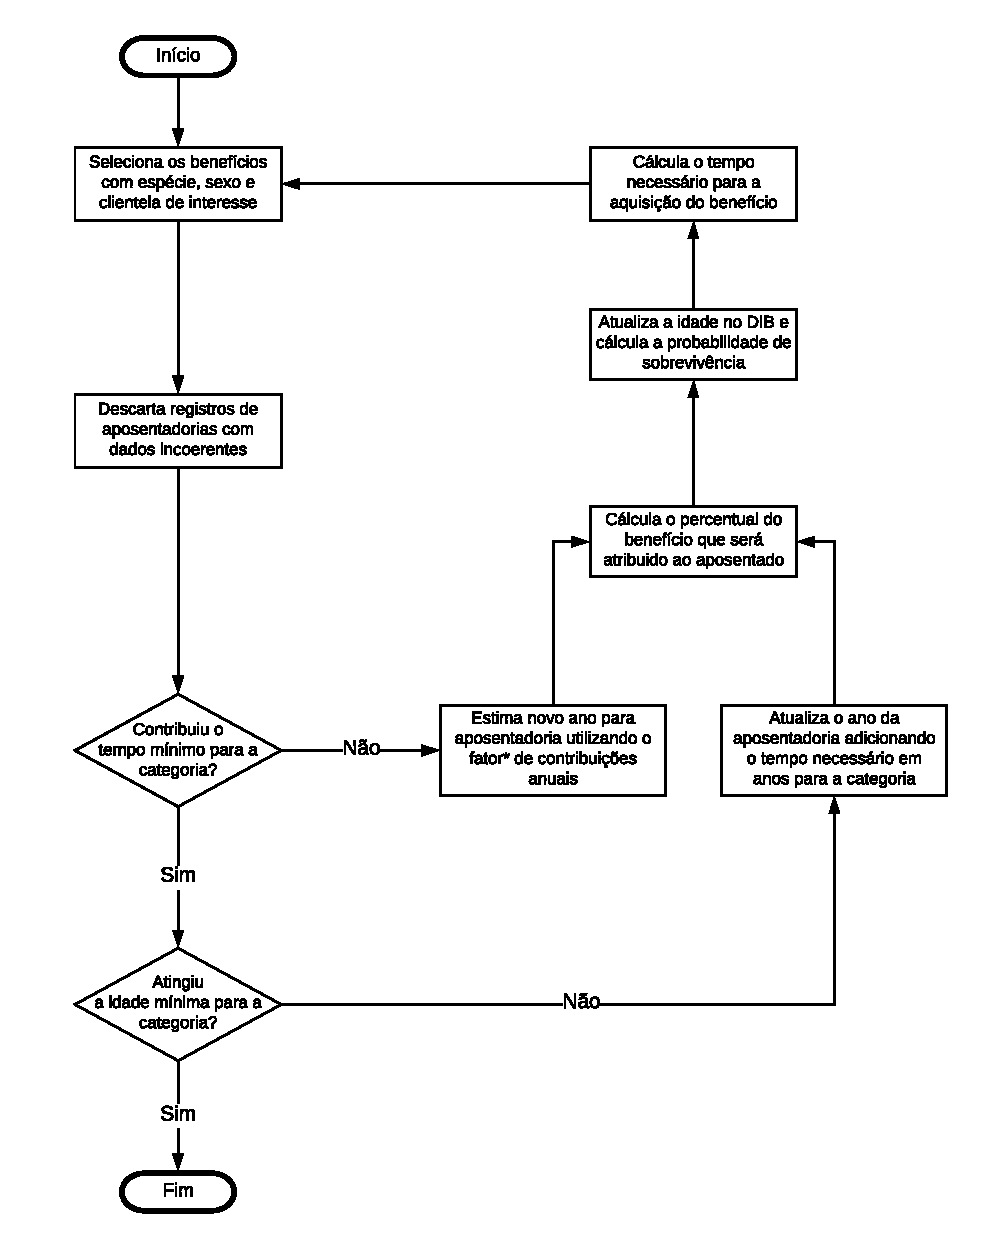
\includegraphics[width=\textwidth]{figs/cap05_fluxograma_reforma_previdencia.pdf}
    \caption*{\footnotesize{Fonte: Elaborado pelo autor}}
    \label{fig:cap05:fluxograma}
\end{figure}

\noindent* O fator de contribuições anuais, destacado no fluxograma, corresponde ao número médio de contribuições anuais, em meses, realizado por cada beneficiário.

\newpage

Inicialmente, houve a leitura e seleção dos registros inerentes a pesquisa, correspondendo aos benefícios das espécies 41, 42, 46, 57, 32 e 92 – aposentadorias por idade, tempo de contribuição, tempo de contribuição especial, tempo de contribuição professor, invalidez previdenciária e invalidez acidentária, respectivamente – para os gêneros masculino e feminino, com clientela urbana e rural, os quais corresponderam a 19.775.373 registros da base de dados. Entretanto, devido a existência de anomalias na idade e tempo de contribuição dos beneficiários, houve uma etapa de triagem nos microdados, reduzindo o universo de interesse em aproximadamente 12,84\% em relação a quantidade anterior, resultando em 17.236.900 registros válidos. 

Após a seleção e remoção de ruídos nos dados de interesse, foram realizadas as simulações propostas. Diante disso, primeiramente, foi verificado se o tempo de contribuição de cada beneficiário correspondia ao tempo mínimo em anos necessário para que a sua categoria obtivesse acesso ao benefício. Caso sim, o registro era selecionado para a próxima etapa, no entanto, caso não, seria estimado e agregado ao beneficiário o tempo em anos necessário para que o mesmo atingisse a regra proposta. Para tal estimativa, levou-se em consideração a dificuldade dos trabalhadores do setor privado se manterem em seus respectivos trabalhos devido, principalmente, as altas taxas de desemprego e informalidade existentes no país \cite{cap04_ref5}. Em seguida, verificou-se se cada beneficiário atingia a idade mínima da sua categoria para a concessão da aposentadoria, acrescentando o tempo a mais que o mesmo haveria de esperar para ter acesso a seu benefício quando necessário.

Dessa forma, após estimar as novas idades e tempo a mais de contribuição, foram calculadas as probabilidades dos beneficiários que não atendiam as regras previstas na PEC 06/2019 estarem vivos na futura concessão dos seus benefícios. Para isso, optou-se por utilizar a projeção populacional realizada pelo IBGE, a qual corresponde a dados de estimativas demográficas a nível nacional classificadas por sexo, idade e clientela, de 2010 a 2060. Assim sendo, a probabilidade de sobrevivência de cada beneficiário pode ser calculada através da Equação~\ref{eq:5.1} abaixo.

\begin{equation}
    prob\_sobrev(i_{proj}, a_{proj}, s) = \frac{POP\_proj(i_{proj}, a_{proj}, s)}{POP\_atual(i_{atual}, a_{atual}, s)}, \left \{a \epsilon \mathbb{I} | 2010 \leq a \leq 2060 \right \}
    \label{eq:5.1}
\end{equation}

\noindent sendo $s$ o sexo do beneficiário e, $i_{proj}$, $i_{atual}$, $a_{proj}$ e $i_{atual}$ a idade na projeção, idade atual, ano na projeção e ano atual, receptivamente. Além disso, as variáveis $POP\_atual$ e $POP\_projetada$ correspondem as populações atuais e projetadas pelo IBGE para cada idade, sexo e ano de interesse.

Por fim, foi calculado o percentual a ser aplicado na média dos salários (contribuições) de cada beneficiário baseando-se nas regras previstas pela reforma da previdência, a qual estipula uma mensalidade 60\% do valor médio, possibilitando um acréscimo de 2\% para cada ano que exceder o tempo mínimo de contribuição . Dessa forma, foram criados sete novos atributos correspondentes a simulação da PEC 06/2019, sendo:

\begin{itemize}
    \item \texttt{PEC6\_GAP\_IDADE}: quantidade de anos a mais que o beneficiário deveria esperar para obter o benefício considerando as novas regras;
    
    \item \texttt{PEC6\_GAP\_CONTRIB}: quantidade de anos a mais que o beneficiário deveria trabalhar para obter o benefício considerando as novas regras;
    
    \item \texttt{PEC6\_GAP}: valor máximo entre o \texttt{PEC6\_GAP\_IDADE} e \texttt{PEC6\_GAP\_CONTRIB};
    
    \item \texttt{PEC6\_ANO\_DIB}: ano mínimo em que o beneficiário terá acesso ao benefício considerando as novas regras;
    
    \item \texttt{PEC6\_IDADE\_DIB}: idade do beneficiário na nova data de início do benefício de aposentadoria considerando as novas regras;
    
    \item \texttt{PEC6\_PROB}: probabilidade de o beneficiário estar vivo no ano em que ficaria elegível para obtenção do benefício;
    
    \item \texttt{PEC6\_PERCENT}: percentual a ser aplicado sobre a média das contribuições para fins de cálculo do valor do benefício.
\end{itemize}

Para o desenvolvimento dessa simulação foi utilizada a linguagem de programação \textit{Python 3}, os \textit{frameworks} de análise de dados \textit{Pandas} e \textit{Numpy} e biblioteca \textit{Psycopg2} responsável por estabelecer uma conexão com o banco de dados PostgreSQL. No repositório do projeto, disponibilizado através da plataforma GitHub\footnote{Disponível em: <https://github.com/andrespp/ds-prev> Acesso em: 3 de Mai, 2020}, pode-se encontrar os \textit{scripts} utilizados em toda simulação com toda a documentação necessária para sua reprodução, apresentando dessa forma um maior grau de detalhamento acerca dos cálculos realizado para cada novo atributo. A Tabela~\ref{tab:cap05:github} descreve a estrutura do projeto e os principais arquivos existentes.

\newpage

\begin{table}[!h]
    \centering
    \caption{Descrição dos principais arquivos do projeto no GitHub referente ao segundo estudo de caso} 
    \begin{tabular}{p{0.22\textwidth}p{0.6\textwidth}}
    \hline
    \textbf{requirements.txt} & arquivo de texto descrevendo todas as dependências e pacotes Python necessários para a execução do projeto.\vspace{3mm}            \\
    \textbf{dataset}          & pasta contendo todos os dados necessários para a execução das análises.\vspace{3mm}                                                \\
    \textbf{doc}              & pasta contendo documentos inerentes a simulação, tais como APES, Ofícios da CPI da Previdência, Taxas, dentre outros. \vspace{3mm} \\
    \textbf{compose}          & pasta contendo os arquivos necessários para levantar a infraestrutura do projeto utilizando a aplicação Docker. \vspace{3mm}       \\
    \textbf{metadata}         & pasta contendo os dicionários e documentações das bases de dados.\vspace{3mm}                                                      \\
    \textbf{dw}               & pasta contendo os arquivos necessários para a criação do data warehouse e realização da simulação.\vspace{3mm}                     \\
    \textbf{analisys}         & pasta com as diversas análises realizadas utilizando a \textit{framework jupyter notebook}.\vspace{3mm}                            \\          
    \textbf{README.md}        & descrição das características e funcionamento do projeto.                                                                           \\\hline
    \end{tabular}
    \caption*{\footnotesize{Fonte: Elaborado pelo autor.}}
    \label{tab:cap05:github}
\end{table}

\newpage

\section{Resultados e Discussão}\label{cap05:resultados}

A partir da estruturação e implementação da arquitetura do \textit{Data Warehouse} para o armazenamento dos microdados previdenciários, e aplicando técnicas/estratégias de ciência de dados para a extração de conhecimento válido acerca da problemática abordada, foi possível realizar a simulação proposta nos objetivos desse estudo. Em vista disso, avaliando as atuais diretrizes do sistema previdenciário nacional, observa-se que as duas principais informações utilizadas para avaliar a viabilidade de um contribuinte se aposentar, tanto no regime atual quanto nas regras da PEC 06/2019, consistem na idade da pessoa e do seu tempo de contribuição para o RGPS. A partir dessas informações, e dependendo das características do trabalho exercido pela contribuinte em questão (trabalhador rural ou urbano, do sexo feminino ou masculino, do tipo professor ou não, dentre outros), este pode passar a ter direito ao benefício da sua aposentadoria.

Dessa forma, como ponto de partida para as análises realizadas, e utilizando os dados reais de aposentadorias concedidas no período analisado , calculou-se a idade média de entrada nos benefícios e o tempo médio em anos de contribuições dos aposentados para o intervalo de tempo analisado, exibindo os resultados nas Tabelas~\ref{tab:cap05:idademedia} e \ref{tab:cap05:contribmedia}. Assim, destaca-se que, de forma geral, os homens se aposentavam em média com 58,24 anos de idade contribuindo com 26,77 anos de trabalho, enquanto as mulheres aposentavam-se com 57,23 anos de idade com uma média de 20,57 anos de trabalho contribuídos para a previdência social. 

\begin{table}[!h]
\centering
\caption{Idade média de entrada em benefício pelas regras atuais do RGPS.}
\renewcommand{\arraystretch}{1.2}
 \newcolumntype{P}[1]{>{\centering\arraybackslash}p{#1}}
\begin{tabular}{P{2cm}P{2cm}P{2cm}P{2cm}P{2cm}P{2cm}}
\toprule[2pt]
 & \textbf{Idade} & \textbf{T.C.} & \textbf{T.C. Esp.} & \textbf{Professor} & \textbf{Rural} \\ \hline
\textbf{Homens} & 65,81 & 53,53 & 48,84 & 56,00 & 60,84 \\ \hline
\textbf{Mulheres} & 61,58 & 51,37 & 49,16 & 50,66 & 56,99 \\ \toprule[2pt]
\end{tabular}
\caption*{\footnotesize{Elaborado pelo autor.}}
\label{tab:cap05:idademedia}
\end{table}

\begin{table}[!h]
\centering
\caption{Tempo (em anos) médio de contribuição pelas regras atuais do RGPS.}
\renewcommand{\arraystretch}{1.2}
 \newcolumntype{P}[1]{>{\centering\arraybackslash}p{#1}}
\begin{tabular}{P{2cm}P{2cm}P{2cm}P{2cm}P{2cm}P{2cm}}
\toprule[2pt]
& \textbf{Idade} & \textbf{T.C.} & \textbf{T.C. Esp.} & \textbf{Professor} & \textbf{Rural} \\ \hline
\textbf{Homens} & 20,35 & 34,52 & 26,02 & 30,90 & 18,39 \\ \hline
\textbf{Mulheres} & 17,27 & 29.37 & 25,86 & 26,55 & 17,82 \\ \hline \toprule[2pt]
\end{tabular}
\caption*{\footnotesize{Elaborado pelo autor.}}
\label{tab:cap05:contribmedia}
\end{table}

Avaliando as Tabelas~\ref{tab:cap05:idademedia} e \ref{tab:cap05:contribmedia}, observa-se que, na média, os homens e mulheres que deram entrada em seus benefícios atendiam as regras expostas na Tabela~\ref{fig:cap05:regraspec}. No entanto, é importante evidenciar que nem todos os trabalhadores que se aposentaram por idade, por exemplo, possuíam o tempo mínimo de contribuição previsto nas regas da PEC 06/2019. Dessa forma, destaca-se que esse período faltando não compreende necessariamente o tempo de trabalho adicional que, na prática, esses contribuintes teriam que cumprir para se aposentarem. Tal fator é justificado pelas elevadas taxas de desemprego e informalidade que impactam diretamente na estabilidade dos trabalhadores do setor privado, dificultando que os mesmos trabalhem formalmente de forma ininterrupta, e consequentemente implicando na idade que estes iriam se aposentar.

Sendo assim, estima-se que os homens aposentados por idade pelas regras atuais necessitariam trabalhar um tempo adicional maior que o previsto, aplicando a mesma analogia para as mulheres e para os demais tipos de aposentadorias consideradas nessa pesquisa. Com isso, utilizando as informações disponibilizadas pelas Tabelas~\ref{tab:cap05:idademedia} e \ref{tab:cap05:contribmedia}, e partindo do princípio de que todos começaram a trabalhar com 18 anos, foi calculado o número médio de contribuições\footnote{Idealmente, o número médio de contribuições por ano deveria ser igual a 12, correspondente a 12 meses de trabalho.} por ano para cada espécie de aposentadoria avaliada, tendo os resultados exibidos na Tabela~\ref{tab:cap05:numcontrib}.

\begin{table}[!h]
\centering
\caption{Número médio de contribuições por ano.}
\renewcommand{\arraystretch}{1.2}
 \newcolumntype{P}[1]{>{\centering\arraybackslash}p{#1}}
\begin{tabular}{P{2cm}P{2cm}P{2cm}P{2cm}P{2cm}P{2cm}}
\toprule[2pt] 
 & \textbf{Idade} & \textbf{T.C.} & \textbf{T.C. Esp.} & \textbf{Professor} & \textbf{Rural} \\ \hline
\textbf{Homens} & 5.11 & 11,66 & 10,13 & 9,76 & 5,15 \\ \hline
\textbf{Mulheres} & 4,76 & 11,57 & 9,96 & 9,76 & 5.49 \\ \hline \toprule[2pt]
\end{tabular}
\caption*{\footnotesize{Fonte: Elaborado pelo autor.}}
\label{tab:cap05:numcontrib}
\end{table}

Tais resultados demonstram que, pelas regras previstas na PEC 06/2019, em algumas situações, o tempo de contribuição necessário para se aposentar, em média, chegaria a equivaler ao dobro do tempo de contribuição restante. Por exemplo, um homem com 65 anos de idade e 15 anos de contribuição, que nas regras atuais consegue a concessão de aposentadoria por idade mas não atende as regras da PEC 06/2019 pela necessidade de 5 anos extras de contribuição, necessitaria trabalhar em média 11,74 anos a mais, visto que a cada ano o mesmo só conseguiria contribuir com 5,11 parcelas, resultando em uma idade de aproximadamente 77 anos ao se aposentar.

Além disso, é importante esclarecer que o número médio de contribuições anuais pode variar de acordo com o cenário econômico vivenciado pelo trabalhador. Crises econômicas e elevações nas taxas de desemprego e informalidade tendem a diminuir as contribuições realizadas, gerando, consequentemente, aumento no tempo adicional de trabalho para as concessões dos benefícios de acordo com as regras da PEC 06/2019.

Paralelamente, uma vez que há modificações nas regras para admissão dos beneficiários, evidencia-se alterações no cenário previdenciário em relação a concessões de aposentadorias. Em geral, as diretrizes atuais especificam que os trabalhadores devem possuir uma idade mínima ou ter um tempo de contribuição mínimo para que o benefício possa ser obtido. Uma vez que as regras propostas pela reforma conciliam ambos os critérios como pré-requisitos para obtenção da aposentadoria, estima-se que uma grande parcela dessas pessoas, possivelmente, não conseguiria mais se aposentar na mesma época em que se aposentou pelas regras atuais.  

Diante disso, utilizando os microdados previdenciários e estratégias computacionais para análises em grandes quantidades de dados\footnote{Devido ao fato da base de dados possuir um volume de informações maior que a quantidade de memória tipicamente disponível em um computador doméstico, optou-se por um processamento em lotes, onde subconjutos dos dados de tamanhos compatíveis com os recursos computacionais disponíveis foram processados sequencialmente. Tal estratégia foi adotada pela natureza dos dados, na qual cada lote é independente do anterior possibilitando dessa forma processamentos isolados.}, foi estimado o percentual de aposentados que teriam acesso aos seus benefícios perante as novas regras propostas. Dessa forma, constatou-se que aproximadamente 83,28\% dos trabalhadores que tiveram suas aposentadorias concedidas durante o intervalo de tempo analisado não teriam acesso a esses benefícios caso a reforma estivesse em vigor desde 1995. A Tabela~\ref{tab:cap05:proporcao} apresenta a proporção de aposentadorias concedidas entre 1995 e 2016 que não atendem as regras pela PEC 06/2019, classificando-as de acordo com seus respectivos sexos, clientelas e espécies do benefício obtido.

\begin{table}[!h]
\centering
\caption{Proporção de pessoas que não atendem as regras da PEC na mesma data que deram entrada nos benefícios com as regras atuais.}
\renewcommand{\arraystretch}{1.2}
 \newcolumntype{P}[1]{>{\centering\arraybackslash}p{#1}}
\begin{tabular}{P{2cm}P{2cm}P{2cm}P{2cm}P{2cm}P{2cm}}
\toprule[2pt] 
 & \textbf{Idade} & \textbf{T.C.} & \textbf{T.C. Esp.} & \textbf{Professor} & \textbf{Rural} \\ \hline
\textbf{Homens} & 51,29\% & 98,57\% & 96,88\% & 77,89\% & 55,77\% \\ \hline
\textbf{Mulheres} & 84,27\% & 98,90\% & 97,91\% & 86,18\% & 87,13\% \\ \toprule[2pt]
\end{tabular}
\caption*{\footnotesize{Fonte: Elaborado pelo autor.}}
\label{tab:cap05:proporcao}
\end{table}

Assim, dos homens que se aposentaram por idade, 51,29\% não teriam conseguido o benefício, enquanto para as mulheres, das que se aposentaram por idade, 84,27\% não teriam conseguido se aposentar. A mesma leitura é aplicada para as pessoas que se aposentaram nas espécies de Aposentadoria por Tempo de Contribuição, Aposentadoria por Tempo de Contribuição Especial, Aposentadoria de Professor e Aposentadoria Rural. Além disso, analisando os resultados, constata-se que as mulheres são as mais impactadas em todas as categorias. Tal fator ocorre, principalmente, devido ao acréscimo na idade mínima – de 60 para 62 anos – necessária para que as pessoas do sexo feminino possam ter acesso aos seus benefícios.

Paralelamente, avaliando os resultados da simulação relacionados ao tempo médio adicional de trabalho, ou espera, necessários para a obtenção da aposentadoria daqueles que não cumpriram as regras previstas na PEC, considerando todo o período de 1995 a 2016, observa-se a existência de duas possíveis situações: (i) pessoas que não atingiram a idade mínima, mas já cumpriram o tempo mínimo de contribuição; (ii) pessoas que atingiram a idade mínima, mas não cumpriram o tempo mínimo de contribuição.

Na primeira situação, temos os trabalhadores que pelas regras atuais obtiveram o benefício da aposentadoria por tempo de contribuição, incluindo os professores que se aposentaram com idade inferior à proposta pela PEC 06/2019. Neste caso, estes trabalhadores necessitariam apenas esperar a idade mínima necessária sem a exigência de continuar contribuindo para a previdência social. Com isso, estimou-se que os homens que se aposentaram por tempo de contribuição deveriam em média esperar aproximadamente mais 11,18 anos até alcançarem a idade mínima, enquanto as mulheres mais 10,31 anos. No caso dos professores e professoras, haveria a necessidade de aguardar em média 5,15 a 7,19 anos, respectivamente. Embora não seja obrigatoriamente exigido que essas pessoas continuassem trabalhando e contribuindo para alcançarem a aposentadoria, provavelmente as mesmas iriam, em detrimento da necessidade de arcar com sua subsistência.

Por outro lado, na segunda categoria encontram-se, no geral, as pessoas que, pelas regras atuais, aposentam-se por idade, incluindo praticamente 100\% dos trabalhadores rurais. Nessa situação específica, é obrigatório que os trabalhadores continuem contribuindo para o sistema previdenciário até cumprirem os requisitos exigidos pela PEC. Desse modo, observa-se que os homens urbanos e rurais que alcançaram os requisitos mínimos para a aposentadoria por idade pelas regras atuais, necessitariam trabalhar, em média, aproximadamente 4,80 e 6,20 anos a mais, respectivamente. Já para as mulheres, haveria a necessidade de acréscimo médio de 3,31 anos no setor urbano e 4,55 anos no rural. Acerca disso, a Tabela~\ref{tab:cap05:sintese} apresenta uma síntese da idade média estimada para as aquisições dos benefícios de aposentadoria pelas regras previstas na PEC 06/2019.


\begin{table}[!h]
\caption{Idade média estimada para a concessão das aposentadorias de acordo as diretrizes previstas pela PEC 06/2019.}
\renewcommand{\arraystretch}{1.2}
 \newcolumntype{P}[1]{>{\centering\arraybackslash}p{#1}}
\begin{tabular}{P{1.6cm}P{3cm}P{3cm}P{3cm}P{3cm}}
\toprule[2pt]
 & \multicolumn{2}{c}{\textbf{Idade  + T.C.}} & \textbf{Professor} & \textbf{Rural} \\ \toprule[2pt]
\multirow{2}{*}{\textbf{Homens}} & \multirow{2}{*}{68,24} & 75,30 – A. Idade & \multirow{2}{*}{60,51} & \multirow{2}{*}{76,76} \\ \cline{3-3}
 &  & 65,03 –  A. T.C. &  &  \\ \hline
\multirow{2}{*}{\textbf{Mulheres}} & \multirow{2}{*}{65,34} & 67,45 – A. Idade & \multirow{2}{*}{57,35} & \multirow{2}{*}{67,14} \\ \cline{3-3}
 &  & 62,03 –  A. TC &  &  \\ \toprule[2pt]
\end{tabular}
\caption*{\footnotesize{Fonte: Elaborado pelo autor.}}
\label{tab:cap05:sintese}
\end{table}

Adicionalmente, diante do que foi exposto, é importante ponderar a possibilidade do contribuinte estar vivo ou não até que o mesmo atinja os requisitos mínimos para a concessão do seu benefício. Diante desse cenário, considerando as datas de cessação de benefícios pela causa de morte, notou-se que aproximadamente 6,97\% (994.173) dos aposentados pelas regras atuais teriam falecido antes de dar entrada no benefício pelas regras previstas na PEC 06/2019. Além disso, utilizando a Equação~\ref{eq:5.1} descrita na metodologia desse estudo de caso, estima-se que dos demais, 509.763 homens e 78.453 mulheres teriam 30\% ou menos de chance de estarem vivos antes da sua elegibilidade para a aposentadoria.

Destaca-se também que a atual reforma previdenciária proposta pelo governo, além de dificultar o acesso dos contribuintes as suas aposentadorias, aplica modificações diretas nos valores de mensalidade repassadas pelo instituto responsável. Nesse contexto, as novas diretrizes preveem um valor de benefício correspondente a 60\% da média total dos salários do trabalhador, com a possibilidade de acréscimo de 2\% a mais para cada ano trabalhado além do mínimo, conforme relatado anteriormente. Dessa forma, observando os aposentados inclusos no espaço amostral analisado, estima-se que apenas 3\% desses receberiam a média integral, ou mais, das suas contribuições. A Tabela~\ref{tab:cap05:percentaplicado} exibe, com maior grau de detalhamento, o percentual médio a ser aplicado para o cálculo do valor dos benefícios, classificando-os por tipo de aposentadoria e sexo.

\begin{table}[!h]
\centering
\caption{Percentual médio a ser aplicado para cálculo do valor do benefício.}
\renewcommand{\arraystretch}{1.2}
 \newcolumntype{P}[1]{>{\centering\arraybackslash}p{#1}}
\begin{tabular}{P{2cm}P{2cm}P{2cm}P{2cm}P{2cm}P{2cm}}
\toprule[2pt] 
 & \textbf{Idade} & \textbf{T.C.} & \textbf{T.C. Esp.} & \textbf{Professor} & \textbf{Rural} \\ \hline
\textbf{Homens} & 0,66 & 0,89 & 0,72 & 0,81 & 0,66 \\ \hline
\textbf{Mulheres} & 0,66 & 0,88 & 0,82 & 0,83 & 0,69 \\ \toprule[2pt]
\end{tabular}
\caption*{\footnotesize{Fonte: Elaborado pelo autor.}}
\label{tab:cap05:percentaplicado}
\end{table}

Além disso, evidencia-se que a parcela de segurados com possibilidade de receber o benefícios integral corresponde, em sua grande maioria, a aposentados por tempo de contribuição. No entanto, a quantidade de concessões de aposentadorias por tempo de contribuição representa apenas 29,24\% do total de concessões. Isto indica que, com a aprovação da PEC, a grande maioria dos aposentados, tenderiam a receber em média um valor abaixo de 70\% da média de todos os salários de contribuição. 

É importante destacar que todos os resultados descritos foram validados e discutidos por especialistas da Associação Nacional dos Auditores Fiscais da Receita Federal (ANFIP), os quais divulgaram um relatório relacionado a temática abordada disponível em \cite{cap05_ref16}.

Por outro lado, avaliando a questão computacional, constatou-se que a abordagem de ciência de dados, aliada a utilização de uma estrutura de \textit{Data Warehouse}, simplificou a execução das consultas, análises e simulação acerca dos microdados previdenciários. Tal fator justifica-se pela natureza dessa arquitetura, a qual objetiva, sobretudo, proporcionar aos usuários e administradores do banco de dados a agregação de diversas dimensões de dados para a abstração de \textit{insights} complexos. 

Além disso, a aplicação de processamento em lotes para a simulação da reforma da previdência - conforme descrito na metodologia deste estudo - possibilitou a efetuação dos cálculos propostos acerca do grande volume de dados utilizados. Tal estratégia, embora não seja uma técnica de paralelização, viabiliza a execução da análise em computadores com recursos limitados, uma vez que executa as tarefas de leitura, processamento e escrita dos resultados acerca de parcelas de dados, descartando, dessa forma, a necessidade de memórias principais com elevadas capacidade de armazenamento, ou utilização do disco rígido como memória auxiliar.

%Acerca dessas análises, e utilizando o conjunto de variáveis existentes na base de dados elaborada, foi desenvolvida uma matriz de correlação, ilustrada na Figura~\ref{fig:cap05:matrixcorr}, objetivando compreender a interdependência existente entre os atributos que nortearam essa pesquisa.

%\begin{figure}[!h]
%    \centering
%    \caption{Matriz de correlação}
%    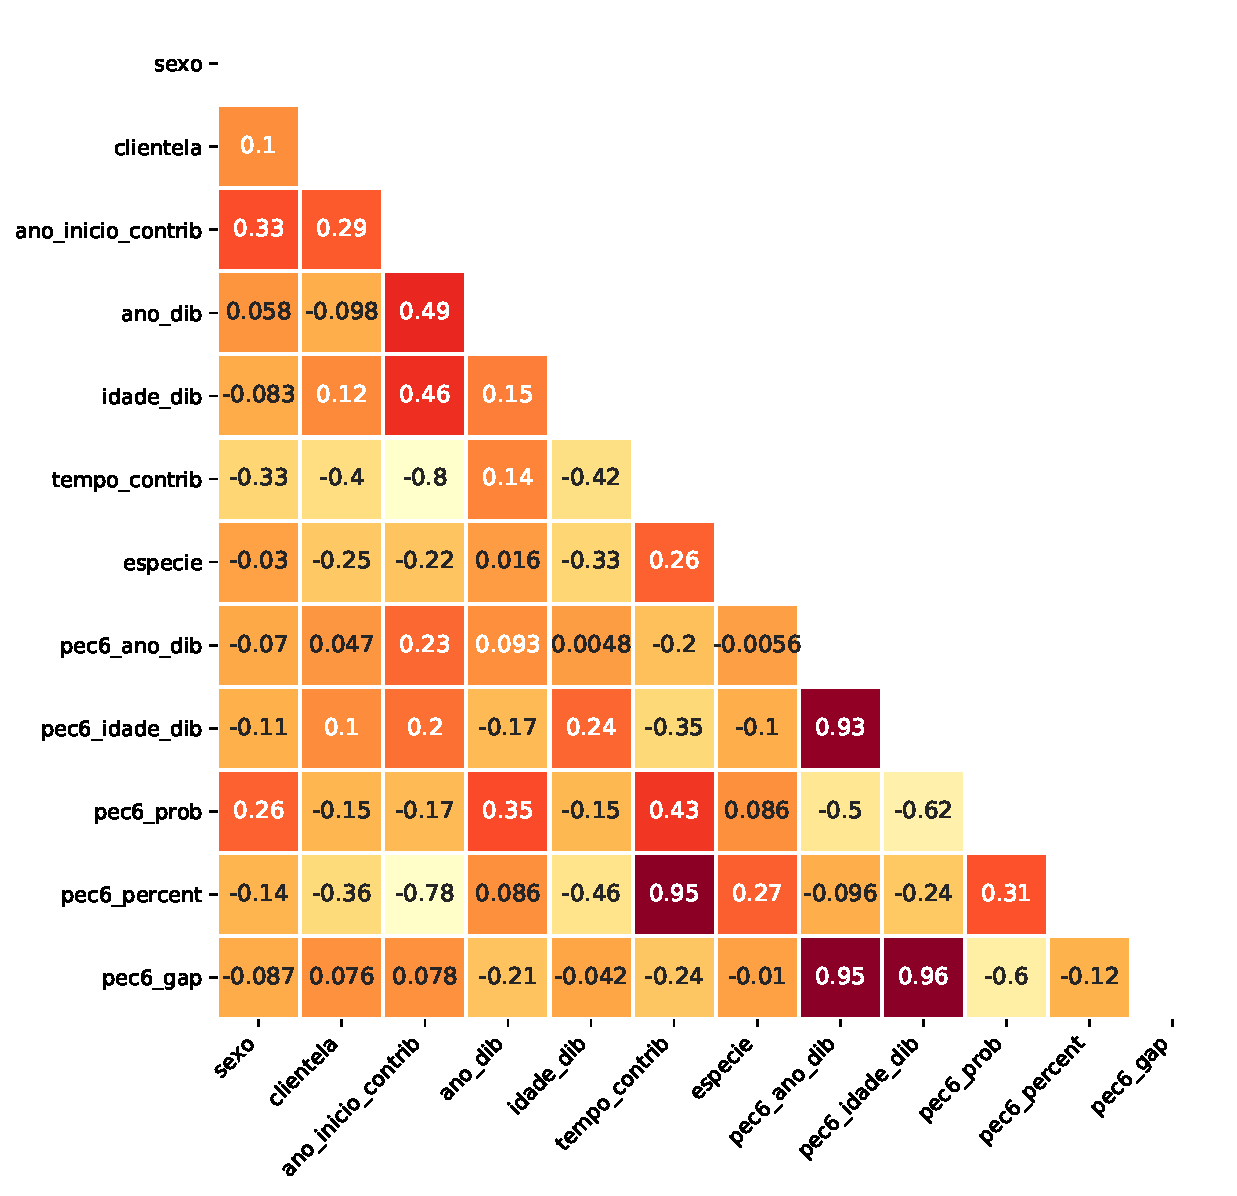
\includegraphics[width=\textwidth]{figs/cap05_corr_matrix.pdf}
%    \caption*{\footnotesize{Fonte: Elaborado pelo autor}}
%    \label{fig:cap05:matrixcorr}
%\end{figure}

\section{Considerações Finais}\label{cap05:conclusoes}

No presente estudo foram realizadas análises acerca dos impactos que a reforma da previdência prevista pela PEC 06/2019 poderia causar no cenário previdenciário nacional, avaliando a série histórica de concessões de aposentadorias entre os anos 1995 e 2016. Nesse contexto, os resultados demonstraram que aproximadamente 78,66\% das aposentadorias concedidas no período analisado não atendem as regras previstas na PEC, fazendo-se necessário um acréscimo em anos de contribuição, ou espera, para que os beneficiários tenham acesso a essas aposentadorias. Paralelamente, foi relatada a dificuldade que os trabalhadores, possivelmente, enfrentariam perante ao novo sistema proposto, uma vez que haverá a necessidade desses manterem-se formais em um mercado de trabalho que não lhe garante total estabilidade.

Adicionalmente, considerando a sobrevida dos aposentados, estimou-se que aproximadamente 6,49\% dos trabalhadores teriam falecido antes de ter acesso ao seu benefício e que 509.763 homens e 78.453 mulheres teriam probabilidade abaixo de 30\% de estarem vivos. Além disso, foi calculado o percentual de repasse que os beneficiários receberiam considerando a regra dos 60\% + 2\% por ano trabalhado, observando que apenas 3\% dos trabalhadores teriam acesso a média integral de todos seus salários, demonstrando a clara dificuldade que as novas regras implicarão para os trabalhadores gozarem desse benefício. 

É evidente que caso as regras previstas pela PEC 06/2019 já estivessem em vigor desde o primeiro ano analisado, o cenário resultante seria diferente do estipulado pelos resultados, afinal, tais regras estimulariam os trabalhadores a terem um perfil diferente no mercado de trabalho. No entanto, é valido considerar os principais desafios que a proposta apresentará para a população, como forma de refletir se essa é melhor alternativa para solucionar o atual problema existente no regime previdenciário nacional.


\chapter{Considerações Finais}\label{cap:conclusao}

A população brasileira está diante de uma possível reforma previdenciária que causará impactos diretos na vida de todos os trabalhadores. Logo, é de extrema importância que a sociedade compreenda as razões que motivaram o governo propor tal medida e os efeitos que tais alterações tendem a causar no cenário social. Paralelamente, é possível observar que o advento da ciência de dados aliada à disseminação de dados abertos governamentais, apresentam-se como importantes ferramentas para a realização de análises cada vez mais complexas e precisas acerca da problemática descrita.

Embora tal abordagem apresente-se em evidência na literatura, destaca-se a ausência de trabalhos que analisem os impactos socioeconômicos relacionados a temática abordada. Isto é, investigando o estado da arte, observou-se uma gama de pesquisas que avaliaram as participações de aposentadorias e pensões na distribuição de renda em um caráter nacional - impossibilitando interpretações em unidades territoriais menores -, e estudos que investigaram os impactos macroeconômicos que a reforma da previdência poderia causar.

Diante disso, esta dissertação visou apresentar dois estudos de caso objetivando, de forma geral, compreender o impacto socioeconômico que o atual cenário previdenciário nacional causa na população, e simular os efeitos que a reforma prevista pela PEC 06/2019 pode provocar na concessão de benefícios. Com isso, a primeira pesquisa utilizou a metodologia de decomposição do índice de Gini e os microdados disponibilizados pelos censos demográficos de 2000 e 2010 para aferir o impacto que as aposentadorias e pensões causam na distribuição de renda dos estados e municípios brasileiros.

Avaliando os resultados, nota-se que houve um aumento da participação dessa parcela de benefícios na composição de rendimentos da população, e uma diminuição no coeficiente de desigualdade econômica. Todavia, embora as aposentadorias e pensões apresentassem caráter regressivo na distribuição de riquezas, observou-se que os benefícios até um salário mínimo colaboravam para a diminuição da concentração de renda. Tal fator destacou-se nos municípios da região nordeste, que, sobretudo, apresentou os menores índices de médias salariais do Brasil. Além disso, destacam-se as interdependências existentes entre as variáveis analisadas, evidenciando a correlação negativa entre a participação dos benefícios avaliados com o índice de Gini, indicando que ao passo que um aumenta o outro diminui.

Por outro lado, o segundo estudo utilizou os microdados de aposentadorias disponibilizados pela CPI da Previdência Social para simular os efeitos que as novas diretrizes, previstas na PEC 06/2019, causariam nos benefícios de 1995 a 2016 se as mesmas já estivessem em vigor na data em que cada aposentadoria foi concedida. Para isso, foram aplicadas estratégias de ciência de dados para facilitar o armazenamento dos dados, consultas e realização de futuras análises. 

Dessa forma, após validar as informações disponibilizadas, observou-se que 83,28\% das aposentadorias concedidas no período analisado não atendiam às novas regras previstas na reforma. Evidenciou-se, então, que a PEC 06/2019, aliada aos elevados índices de informalidade existentes no Brasil, dificultaria o acesso a tais benefícios, dado a dificuldade que trabalhadores da RGPS tem em manterem-se estáveis em seus empregos. Além disso, estimou-se que aproximadamente 6,48\% dos beneficiários teriam falecido antes de dar entrada nas suas aposentadorias, e que somente 3\% do total receberiam a média integral, ou mais, das suas contribuições como mensalidade.

Embora não tenham sido aplicadas técnicas de inteligência computacional nas análises realizadas, destaca-se a eficiência de utilizar ciência de dados em bases de dados abertas governamentais, uma vez que tal estratégia possibilitou a extração de conhecimento válido acerca de dados sem representatividade, podendo, dessa forma, servir como ferramenta para auxiliar possíveis tomadas de decisão em gestão pública. 

Com objetivo de promover um trabalho colaborativo, foram disponibilizados todos os \textit{scripts}, ferramentas e dados utilizados nessa dissertação na plataforma GitHub, possibilitando esforços da comunidade cientifica para o enriquecimento nas análises realizadas. Com isso, devido ao fato de compreender um campo interdisciplinar, a Previdência Social possibilita que pesquisadores de diversas áreas desenvolvam alternativas para o debate com diferentes óticas, possibilitando, dessa forma, a elaboração políticas públicas cada vez mais justas e eficientes diante do cenário brasileiro.

\section{Dificuldades Encontradas}

Durante o desenvolvimento do trabalho foram encontradas uma série de dificuldades relacionadas, principalmente, a dificuldade de acesso a informações e granularidade dos dados disponibilizados.

Dentre as principais dificuldades encontradas durante a realização deste trabalho, destacam-se:

\begin{itemize}
    \item Ausência de microdados atualizados dos rendimentos de aposentadorias e pensões acerca dos municípios brasileiros, impossibilitando a realização de investigações mais precisas da atual participação que esses benefícios tem na distribuição de renda.
    
    \item Ausência das identificações de estados e municípios nos microdados da CPI da Previdência, impossibilitando análises territoriais mais precisas dos impactos que a PEC 06/2019 pode causar.
    
    \item Ausência das datas de cessação dos benefícios contidos na base da CPI da Previdência, impossibilitando uma avaliação histórica de benefícios ativos.
    
    \item A granularidade das informações disponibilizadas pelo AEPS, divulgando informações agregadas que impossibilitam análises mais detalhadas e complexas.
\end{itemize}


\section{Trabalhos Futuros}
 
Esta pesquisa encontra-se em desenvolvimento, possibilitando a realização de novas análises e discussões acerca da temática abordada. Dessa forma, os seguintes itens estão em processo de aperfeiçoamento e serão publicados em trabalhos futuros:

\begin{itemize}
    \item A exploração complementar da metodologia de decomposição do índice de Gini, efeitos composição e concentração, em outras subcategorias de salários (2, 3 e 4 salários mínimos, por exemplo), para avaliar de forma mais precisão a participação que as aposentadorias e pensões possuem na distribuição de riquezas da população.
    
    \item A aplicação de métodos estatísticos espaciais, como a varredura espacial de Kulldorff, afim de detectar regiões de \textit{clusters} acerca da das variáveis analisadas.
    
    \item A aplicação de técnicas de inteligência computacional, como Redes Bayesianas, para identificar as principais variáveis que influenciam na distribuição de renda da população.
    
    \item Utilizar as taxas de informalidade e desemprego para aferir, de forma mais precisa, o comportamento que as concessões de aposentadorias e pensões teriam se as regras previstas pela PEC 06/2019 já estivessem em vigor.
    
    \item Avaliar os impactos que a reforma da previdência causaria na distribuição de renda da população brasileira utilizando o índice de Gini e outras fontes de dados, como por exemplo a PNAD. 
\end{itemize}

% ----------------------------------------------------------
% ELEMENTOS PÓS-TEXTUAIS (Referências, Glossário, Apêndices)
% ----------------------------------------------------------
\postextual

% Referências bibliográficas
\bibliography{bibliografia}

% Glossário (Consulte o manual)
%\glossary

% Apêndices
% ----------------------------------------------------------
% Apêndices
% ----------------------------------------------------------

% ---
% Inicia os apêndices
% ---
\begin{apendicesenv}

% Imprime uma página indicando o início dos apêndices
\partapendices

% ----------------------------------------------------------
\chapter{Atributos dos Microdados Disponibilizados pela CPI da Previdência}\label{apendice:a}
% ----------------------------------------------------------


\begin{table}[!h]
\renewcommand{\arraystretch}{1.3}
\resizebox{\textwidth}{!}{
\begin{tabular}{|c|c|cl}
\hline
\textbf{Campo} & \multicolumn{1}{l|}{\textbf{Descrição Campo}} & \multicolumn{1}{c|}{\textbf{Código}} & \multicolumn{1}{l|}{\textbf{Descrição Código}} \\ \hline
\multirow{8}{*}{ESPECIE} & \multirow{8}{*}{Espécie do Benefício} & \multicolumn{1}{c|}{31} & \multicolumn{1}{l|}{Auxilio doença previdenciário} \\ \cline{3-4} 
 &  & \multicolumn{1}{c|}{32} & \multicolumn{1}{l|}{Aposentadoria por invalidez previdenciária} \\ \cline{3-4} 
 &  & \multicolumn{1}{c|}{41} & \multicolumn{1}{l|}{Aposentadoria por idade} \\ \cline{3-4} 
 &  & \multicolumn{1}{c|}{42} & \multicolumn{1}{l|}{Aposentadoria por tempo de serviço previdenciária} \\ \cline{3-4} 
 &  & \multicolumn{1}{c|}{46} & \multicolumn{1}{l|}{Aposentadoria por tempo de serviço especial} \\ \cline{3-4} 
 &  & \multicolumn{1}{c|}{57} & \multicolumn{1}{l|}{Aposentadoria por tempo de serviço de professor} \\ \cline{3-4} 
 &  & \multicolumn{1}{c|}{91} & \multicolumn{1}{l|}{Auxílio doença acidentário} \\ \cline{3-4} 
 &  & \multicolumn{1}{c|}{92} & \multicolumn{1}{l|}{Aposentadoria por invalidez por acidente do trabalho} \\ \hline
DIB & Data de Início do Benefício &  &  \\ \cline{1-2}
DDB & Data de Despacho do Benefício &  &  \\ \cline{1-2}
MOT\_CESSACAO & Motivo de Cessação * &  &  \\ \cline{1-2}
ULT\_COMPET\_MR & \begin{tabular}[c]{@{}c@{}}Competência da Cálculo da Última\\ Mensalidade Reajustada\end{tabular} &  &  \\ \cline{1-2}
VL\_MR & \begin{tabular}[c]{@{}c@{}}Valor da Última Mensalidade\\ Reajustada\end{tabular} &  &  \\ \cline{1-2}
DT\_NASC & Data de Nascimento do Titular &  &  \\ \cline{1-2}
VL\_RMI & Valor da Renda Mensal Inicial &  &  \\ \hline
\multirow{3}{*}{CLIENTELA} & \multirow{3}{*}{Clientela} & \multicolumn{1}{c|}{1} &
\multicolumn{1}{l|}{Masculino} \\ \cline{3-4} 
 &  & \multicolumn{1}{c|}{3} & \multicolumn{1}{l|}{Feminino} \\ \cline{3-4} 
 &  & \multicolumn{1}{c|}{9} & \multicolumn{1}{l|}{Ignorado} \\ \hline
\multirow{16}{*}{SITUACAO} & \multirow{16}{*}{Situação do Benefício} & \multicolumn{1}{c|}{0} & \multicolumn{1}{l|}{Ativo} \\ \cline{3-4} 
 &  & \multicolumn{1}{c|}{2} & \multicolumn{1}{l|}{Cessado} \\ \cline{3-4} 
 &  & \multicolumn{1}{c|}{3} & \multicolumn{1}{l|}{Suspenso} \\ \cline{3-4} 
 &  & \multicolumn{1}{c|}{4} & \multicolumn{1}{l|}{Suspenso por Marca de Erro} \\ \cline{3-4} 
 &  & \multicolumn{1}{c|}{5} & \multicolumn{1}{l|}{Cessado por Cess do Titular Proprio (Pa)} \\ \cline{3-4} 
 &  & \multicolumn{1}{c|}{7} & \multicolumn{1}{l|}{Bloqueado Pelo Controle de Pagamento} \\ \cline{3-4} 
 &  & \multicolumn{1}{c|}{8} & \multicolumn{1}{l|}{Cessado Pelo Sistema de Obitos da Dtp} \\ \cline{3-4} 
 &  & \multicolumn{1}{c|}{10} & \multicolumn{1}{l|}{Recebendo Mensalid de Recuper 6 Meses} \\ \cline{3-4} 
 &  & \multicolumn{1}{c|}{11} & \multicolumn{1}{l|}{Recebendo Mensalid de Recuper 18 Meses} \\ \cline{3-4} 
 &  & \multicolumn{1}{c|}{12} & \multicolumn{1}{l|}{Suspenso Pelo Sistema de Revisao Rur/Urb} \\ \cline{3-4} 
 &  & \multicolumn{1}{c|}{16} & \multicolumn{1}{l|}{Beneficio Suspenso Pela  Auditoria} \\ \cline{3-4} 
 &  & \multicolumn{1}{c|}{17} & \multicolumn{1}{l|}{Beneficio Cessado Pela Inspetoria} \\ \cline{3-4} 
 &  & \multicolumn{1}{c|}{18} & \multicolumn{1}{l|}{Beneficio Cessado Pela Auditoria} \\ \cline{3-4} 
 &  & \multicolumn{1}{c|}{22} & \multicolumn{1}{l|}{Cessado Pela Revisao Rural/95} \\ \cline{3-4} 
 &  & \multicolumn{1}{c|}{23} & \multicolumn{1}{l|}{Susp. Pelo Sistema de Obitos da Dataprev} \\ \cline{3-4} 
 &  & \multicolumn{1}{c|}{24} & \multicolumn{1}{l|}{Cancelado Pela Auditoria} \\ \hline
DT\_OBITO & Data de Óbito &  &  \\ \cline{1-2}
TEMPO\_CONTRIB & \multicolumn{1}{c|}{\begin{tabular}[c]{@{}c@{}}Tempo de Contribuição, em Anos,\\ do Titular\end{tabular}} &  &  \\ \cline{1-2}
IDADE\_DIB & \multicolumn{1}{c|}{Idade na DIB do Titular} &  &  \\ \cline{1-2}
\end{tabular}}
\end{table}

* Códigos com os motivos de cessação listados a seguir.

\newpage

\begin{table}[!ht]
\renewcommand{\arraystretch}{1.5}
\resizebox{\textwidth}{!}{
\begin{tabular}{|c|c|c|c|}
\hline
\textbf{Código} & \textbf{Descrição} & \textbf{Código} & \textbf{Descrição} \\ \hline
2 & NAO COMPROVACAO DE FE DE VIDA & 51 & CESSACAO POR REVISAO RURAL/95 \\ \hline
3 & CESSACAO POR SUSPEITA DE OBITO/SIM & 52 & ERRO ADM. INFORMADO PELA AUDITORIA \\ \hline
4 & REVBPC NAO LOCALIZ. DO BENEFICIARIO & 53 & FRAUDE INFORMADA PELA AUDITORIA \\ \hline
5 & NAO APRES. DE DOCS. OBRIGATORIA & 54 & LIMITE MEDICO INFORMADO P/ PERICIA \\ \hline
6 & NAO ATENDIMENTO A CONVOC.POSTO & 55 & IRREGULARID./ERRO MEDICO-PERICIAL \\ \hline
7 & BPC\textgreater{}2 ANOS - APRENDIZ C/ DEFIC. & 56 & RECUP.LESAO C/ DESCARAC. DO BENEF. \\ \hline
8 & BENEFICIO CONCEDIDO COM CESSACAO DA DIB & 57 & CESS. DE AUXILIO RECLUSAO POR FUGA \\ \hline
9 & DCA ACP2005.33.00.020219-8 & 58 & BENEFICIO C/DCI C/ MAIS DE 60 DIAS \\ \hline
10 & CESSACAO POR SUSPEITA DE OBITO & 59 & CESSADO, DIVERGENCIA DADOS CNIS \\ \hline
11 & CESSACAO POR NAO COMPARECIMENTO AO CENSO & 60 & CESS.DE BENEFICIO FORA DE CADASTRO \\ \hline
12 & LIMITE MEDICO & 61 & RECUSA AO PROGR. REABILIT. PROFIS. \\ \hline
13 & OBITO DO TITULAR DO BENEFICIO & 62 & REVBPC N+DEF LON PZ/R\textgreater{}1/4S \\ \hline
14 & CESSACAO P/ACAO REVISIONAL COMPARTILHADA & 63 & CESSACAO P/ FALTA DE DIGITALIZACAO \\ \hline
15 & OPCAO CONCESSAO BENEFICIO PREVIDENCIARIO & 64 & OBITO SEGURADO INSTIT.AUX.RECLUSAO \\ \hline
16 & CASAMENTO & 65 & BENEF. SUSPENSO POR MAIS DE 6 MESES \\ \hline
17 & REAPARECIMENTO DO INSTITUIDOR & 66 & VOLTA TRABALHO-ATIV.INSALUBRE(B46) \\ \hline
18 & DESISTENCIA BPC-LOAS PELO TITULAR & 67 & CESSACAO POR CONCESSAO DE B80 \\ \hline
19 & CESS. PA DEVIDO CESS. BENEF. INST. & 68 & REMUNERACAO APOS A DIB \\ \hline
20 & DESISTENCIA ESCRITA TITULAR DO BENEFICIO & 69 & ALTA MEDICA \\ \hline
21 & TRANSFORMACAO B87 EM B88 & 70 & RETORNO VOLUNTARIO AO TRABALHO \\ \hline
22 & PRORROGACAO DE BENEFICIO ANTERIOR & 71 & ERRO TECNICO \\ \hline
23 & CONCES. APOSENT. P/RECLUSO & 72 & NAO COMPARECIMENTO \\ \hline
24 & SUSPENSAO 64 P/MAIS 6MESES & 73 & RET./PERMANENC.NA ATIV.COND.ESPEC. \\ \hline
25 & NB TRANSITADO JULG/REV.ADM & 74 & CANCELAMENTO POR FRAUDE/AUDITORIA \\ \hline
26 & RENDA PER CAPITA - REVBPC & 75 & CANCELAMENTO P/IRREGULARIDADE/AUDITORIA \\ \hline
27 & PM DENEGATORIA - REVBPC & 76 & CANCELAMENTO P/ERRO ADM.MEDICO/AUDITORIA \\ \hline
28 & TRANSFORMACAO PARA OUTRA ESPECIE & 77 & IRREGULARIDADE DETECTADA PELA AUDITORIA \\ \hline
29 & CONCESSAO DE OUTRO BENEFICIO & 78 & CESS. DE B80 C/CONTRATO TEMPORARIO \\ \hline
30 & CONSTATACAO DE FRAUDE & 79 & CESSACAO DE B80 (120/134 DIAS) \\ \hline
31 & CONSTATACAO IRREGULAR./ERRO ADM. & 80 & ABORTO NAO CRIMINOSO \\ \hline
32 & DECISAO DE CESSACAO POR RECURSO & 81 & OBITO INFORMADO PELA REVBPC \\ \hline
33 & DECISAO JUDICIAL & 82 & CESSACAO DE B80 (60 DIAS) \\ \hline
34 & VOLTA AO TRABALHO & 83 & CESSACAO DE B80 (30 DIAS) \\ \hline
35 & BENEFICIO SEM DEPENDENTE VALIDO & 84 & CESSACAO - OPCAO RECEB. PELO M.  EXERCITO \\ \hline
36 & ACUMULACAO INDEVIDA DE BENEFICIOS & 85 & BENEFICIO COM NIT ERRADO \\ \hline
37 & SUSP SISOBI MAIS 6 MESES & 86 & CESSACAO B94/95 PARECER MEDICO  CONTRARIO \\ \hline
38 & CESSACAO ABONO P/ CONCES. APOSENT. & 87 & CESSACAO ACUMULACAO INDEVIDA REV. 2003 \\ \hline
39 & NAO ATENDIMENTO CONVOCACAO INSPET. & 88 & REVBPC N HA+DEF LONG PZ \\ \hline
40 & CESS.P/ RECUP.TOTAL DENTRO 5 ANOS & 89 & CESSACAO AMPARO LEI 10559/02. \\ \hline
41 & CESS.P/ RECUP. PARCIAL APOS 5 ANOS & 90 & CESSACAO DE PA DEVIDO DATA LIMITE \\ \hline
42 & CESSADO P/ SIST. DE OBITOS(SISOBI) & 91 & REVISAO DE ACORDAO \\ \hline
43 & AUX.RECL.-CUMPR.PENA,CONDIC.,ALBERG. & 92 & LIMITE INDEFINIDO S/CONCESSAO DE B32/92 \\ \hline
44 & AUX.DOENCA NAO COMPAREC. A PERICIA & 93 & CESSACAO BATIMENTO FUNASA \\ \hline
45 & CESS. BENEFICIO - RECIPROCA & 94 & ALTA VOLUNTARIA \\ \hline
46 & ESTATUTARIO TRANSF. P/ORGAO ORIGEM & 95 & NAO COMPARECIMENTO A REABILITACAO PROF. \\ \hline
47 & CESS. DEVIDO PERDA QUALID. DEPEND. & 96 & TRANSFERENCIA P/ORGAO ORIGEM LEI 8878/94 \\ \hline
48 & BENEF. CESSADO NO SISTEMA ANTIGO & 97 & COMPROVADA MA FE DO BENEFICIARIO \\ \hline
49 & OBITO INFORMADO PELA AUDITORIA & 98 & CESSACAO POR LEI \\ \hline
50 & CONCESSAO DE AUXILIO FUNERAL (PAB) & 99 & OBITO DEPENDENTE INFORM.  P/CENSO(HIPNET) \\ \hline
\end{tabular}}
\end{table}
% ----------------------------------------------------------
%\chapter{Perceba que o texto do título desse segundo apêndice é bem grande}
% ----------------------------------------------------------
%\lipsum[51-53] % Texto qualquer. REMOVER!!

\end{apendicesenv}
% ---

% Anexos
%% ----------------------------------------------------------
% Apêndices
% ----------------------------------------------------------

% ---
% Inicia os anexos
% ---
\begin{anexosenv}

% Imprime uma página indicando o início dos anexos
\partanexos

% ---
\chapter{Nome do Primeiro Anexo}
% ---
\lipsum[30] % Texto qualquer. REMOVER!!

% ---
\chapter{Nome de Outro Anexo}
% ---

\lipsum[32] % Texto qualquer. REMOVER!!

\end{anexosenv}

% Índice remissivo (Consultar manual)
%\phantompart
%\printindex

\end{document}
